% =========================================================
\chapter{Resultados y discusión}
\label{chapter:resultados}
% =========================================================

% Párrafo introductorio del capítulo
% TODO: Introducir brevemente la estructura del capítulo y recordar al lector
%   los dos ejes de análisis: (1) efecto del balanceo sobre el conjunto de
%   entrenamiento y (2) efecto sobre la predicción LSTM. Mencionar que el
%   análisis estadístico (Friedman + Nemenyi) opera sobre los resultados
%   del segundo eje, y que el primer eje es condición necesaria para
%   interpretar correctamente el segundo. Aprox. 3-4 frases.
Este capítulo presenta y discute los resultados del trabajo en dos bloques complementarios. El primero analiza cómo cada técnica de balanceo modifica el conjunto de entrenamiento —su tamaño y su distribución glucémica y demográfica— y argumenta por qué esta información es imprescindible para interpretar correctamente los resultados de predicción. El segundo bloque evalúa el impacto de dichas modificaciones sobre el rendimiento del modelo LSTM, tanto en términos de métricas agregadas (RMSE, MAE) como en términos clínicos (distribución de zonas del Clarke Error Grid). A lo largo de ambos bloques se da prioridad a la interpretación clínica sobre la estadística pura, en línea con el objetivo principal del trabajo.

% =========================================================
\section{Efecto del balanceo sobre el conjunto de entrenamiento}
\label{sec:efecto_balanceo_trainset}
% =========================================================

Antes de evaluar el impacto de las técnicas de balanceo sobre el rendimiento
predictivo del modelo LSTM, es necesario caracterizar con precisión qué hace
cada técnica sobre el propio conjunto de entrenamiento. Esta caracterización
previa no es un paso auxiliar: es una condición metodológica indispensable para
interpretar correctamente cualquier diferencia de rendimiento entre condiciones.
Sin ella, una mejora observada tras aplicar \textit{oversampling} podría
atribuirse al reequilibrio demográfico cuando en realidad se debe al aumento
del volumen de datos; del mismo modo, un deterioro tras \textit{undersampling}
podría confundirse con un efecto del desbalanceo residual cuando la causa real
es la pérdida de información. Esta sección documenta, para cada técnica,
\textit{dataset} y dimensión demográfica, dos propiedades del conjunto de
entrenamiento resultante: su tamaño y la distribución glucémica de sus
particiones demográficas. Ambas propiedades son necesarias para establecer
una relación causal entre la intervención de balanceo y sus efectos sobre
la predicción.

Las técnicas de balanceo no son equivalentes entre sí ni en los datos que
producen ni en los mecanismos por los que lo hacen. Un modelo entrenado con
un conjunto sometido a \textit{undersampling} ve sustancialmente menos datos
que uno entrenado con el original, mientras que uno entrenado con
\textit{oversampling} ve más ---y parte de esos datos son sintéticos o
duplicados---. Esta heterogeneidad es especialmente pronunciada en DiaTrend,
donde el ratio de desequilibrio demográfico por edad es de 38:1
(véase sección~\ref{subsec:eda_demografico}), lo que hace que las mismas
técnicas produzcan variaciones de tamaño mucho más extremas que en
T1DiabetesGranada o REPLACE-BG. El análisis que sigue está estructurado
en dos subsecciones: la primera cuantifica el impacto sobre el tamaño del
conjunto de entrenamiento; la segunda analiza cómo cambia la distribución
glucémica intra-grupo tras el balanceo, que es el mecanismo por el cual
el reequilibrio demográfico puede influir en el aprendizaje del modelo.
% ---------------------------------------------------------
\subsection{Impacto sobre el tamaño del conjunto de entrenamiento}
\label{subsec:impacto_tamaño}
% ---------------------------------------------------------
% FIGURAS:
%   - balancing/FIG-B3  trainsize_bars_age.pdf   → tamaño train por técnica, dim. edad
%   - balancing/FIG-B3  trainsize_bars_sex.pdf   → tamaño train por técnica, dim. sexo
%
% AMBAS figuras van juntas: muestran media ± SD sobre los 5 folds.
% La línea discontinua del original sirve como referencia visual.
%
% PRINCIPIO: figura → texto que la comenta.

\begin{figure}[H]
    \centering
    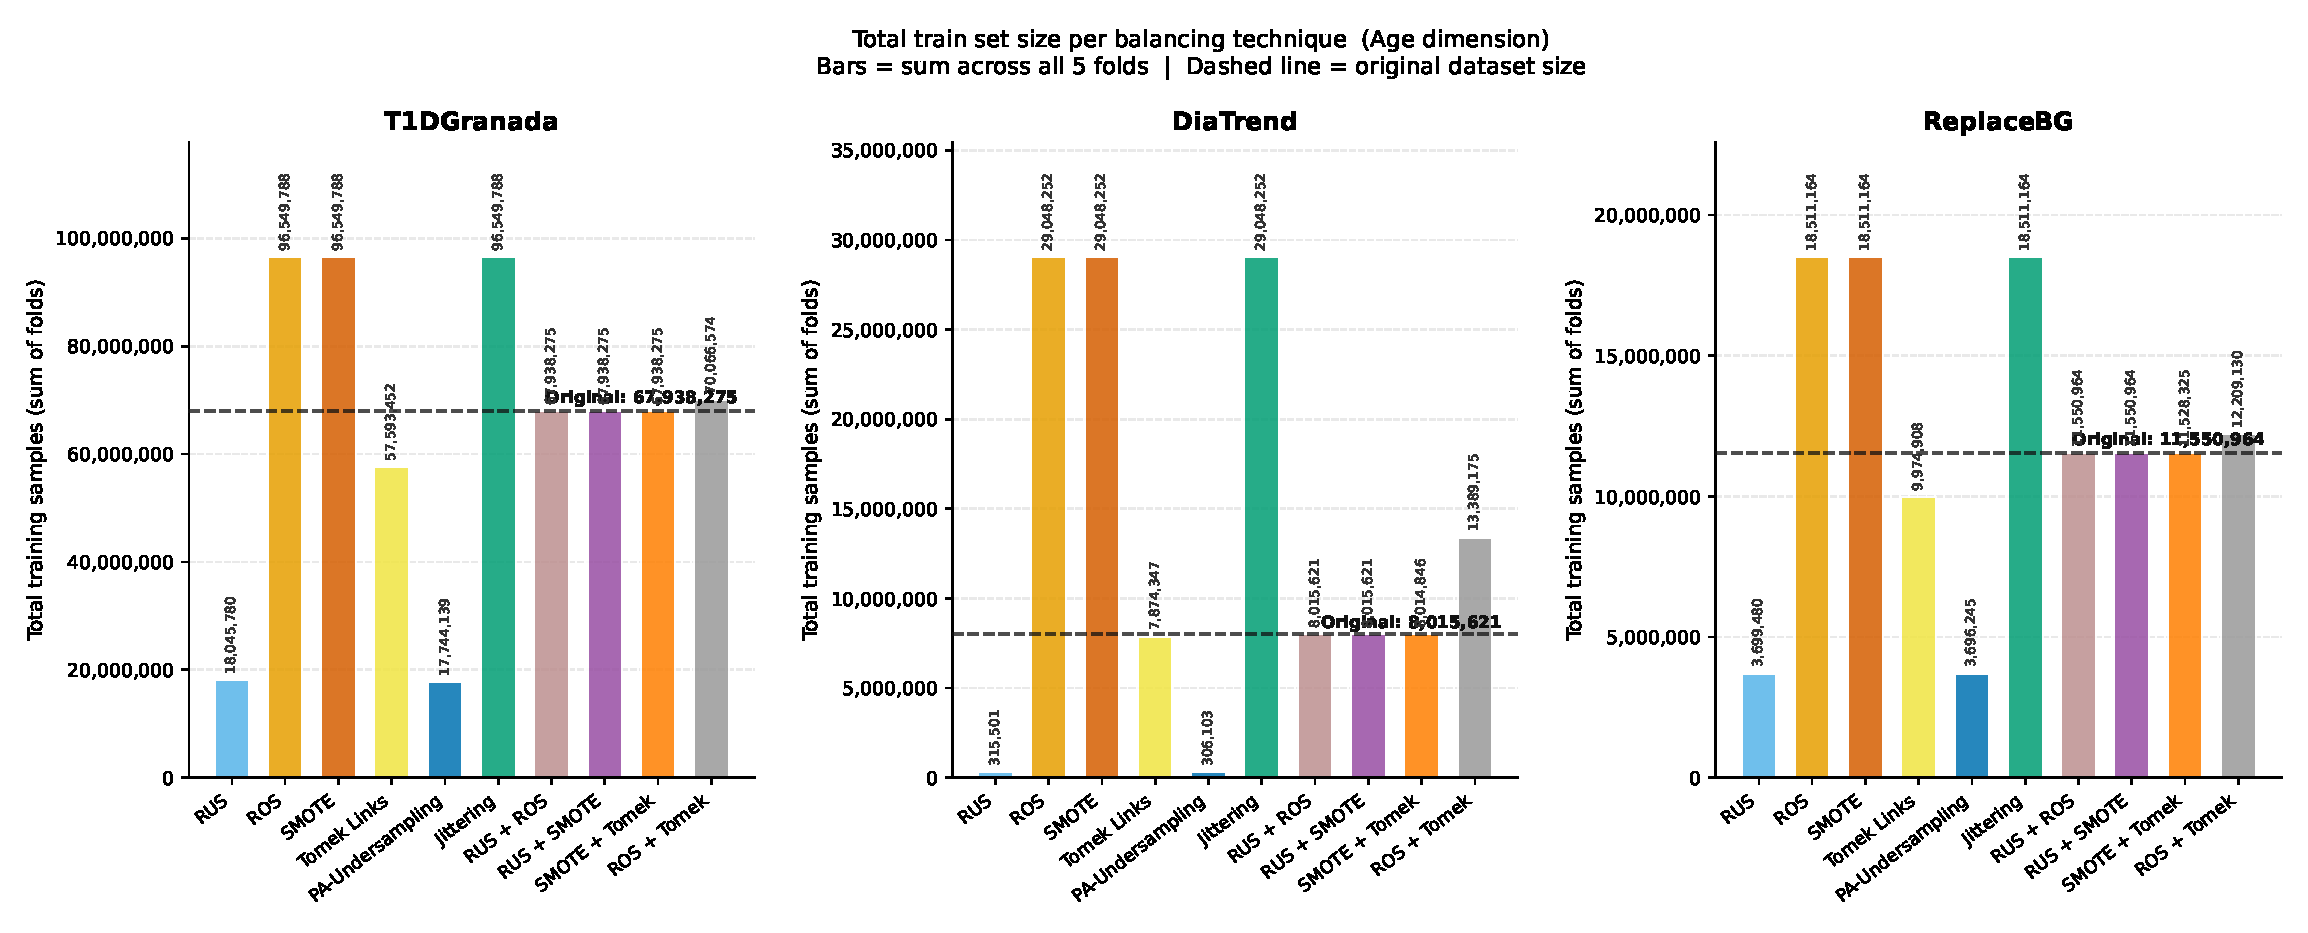
\includegraphics[width=\textwidth]{../../analysis_relief/outputs_clinical/trainsize_bars_age}
    \caption{Tamaño medio del conjunto de entrenamiento (número de ventanas,
             media $\pm$ SD sobre los 5 \textit{folds}) por técnica de balanceo
             y \textit{dataset}, para la dimensión demográfica \textbf{edad}.
             La línea discontinua indica el tamaño medio del conjunto original
             sin balancear.}
    \label{fig:trainsize_age}
\end{figure}

Las figuras~\ref{fig:trainsize_age} y~\ref{fig:trainsize_sex} muestran el tamaño
medio del conjunto de entrenamiento tras aplicar cada técnica, separadas por
dimensión demográfica (edad y sexo respectivamente). El patrón general es
consistente entre dimensiones, pero la magnitud de las variaciones difiere
sustancialmente entre \textit{datasets} en función de su ratio de desequilibrio.

\paragraph{Técnicas de reducción (RUS y PA-Undersampling).}
En la dimensión edad, RUS y PA-Undersampling producen las reducciones más drásticas
en DiaTrend, donde el ratio de desequilibrio entre grupos etarios es extremo
(véase sección~\ref{subsec:eda_demografico}): el conjunto de entrenamiento cae
hasta 63\,100 y 61\,220 ventanas respectivamente, frente a un original de
1\,603\,124 ---una reducción del 96\,\%---. En T1DiabetesGranada la reducción
es moderada (de 13\,587\,655 a $\approx$3\,600\,000, un 73\,\% menos) y en
REPLACE-BG es la más contenida (de 2\,310\,192 a $\approx$740\,000, un 68\,\%).
En la dimensión sexo, donde el desequilibrio es mucho menor en todos los
repositorios, la reducción por RUS es notablemente más moderada: T1DiabetesGranada
pasa de 13\,587\,655 a 12\,769\,338 (solo un 6\,\% menos), y REPLACE-BG
prácticamente no varía (de 2\,310\,192 a 2\,185\,953). DiaTrend sigue siendo el
caso más extremo incluso en sexo, con una caída hasta 666\,551 ventanas (58\,\%
de reducción), reflejo de que incluso el desequilibrio de sexo en ese repositorio
es más pronunciado que en los otros dos.

\paragraph{Técnicas de aumento (ROS, SMOTE, Jittering).}
En la dimensión edad, ROS, SMOTE y Jittering multiplican el tamaño del train en
DiaTrend por un factor de $\approx$3{,}6$\times$ (hasta 5\,809\,650 ventanas),
el más alto de todos los repositorios. En T1DiabetesGranada el incremento es
proportionalmente más contenido ($\approx$19\,310\,000, un 42\,\% sobre el
original), y en REPLACE-BG el aumento es de solo un 60\,\% (hasta 3\,702\,232).
Tomek Links es la excepción dentro de este grupo: al limitarse a eliminar puntos
fronterizos, reduce ligeramente el tamaño respecto al original en todos los casos
(1\,574\,869 en DiaTrend, 11\,518\,690 en T1DiabetesGranada, 1\,994\,981 en
REPLACE-BG), lo que lo acerca en comportamiento a las técnicas de reducción.
En la dimensión sexo el patrón se suaviza considerablemente: el factor de aumento
máximo en DiaTrend es $\approx$1{,}6$\times$ (2\,539\,697 frente a 1\,603\,124),
y en T1DiabetesGranada y REPLACE-BG el incremento es marginal (inferior al 6\,\%).

\paragraph{Técnicas híbridas (RUS+ROS, RUS+SMOTE, SMOTE+Tomek, ROS+Tomek).}
Por diseño, RUS+ROS y RUS+SMOTE producen conjuntos de exactamente el mismo tamaño
que el original en todos los \textit{datasets} y ambas dimensiones. SMOTE+Tomek
mantiene el tamaño original en T1DiabetesGranada y REPLACE-BG, pero en DiaTrend
queda ligeramente por debajo (1\,602\,969 frente a 1\,603\,124 en edad), confirmando
el efecto de la fase de limpieza de Tomek ya descrito en la
sección~\ref{subsec:modos_pipeline}. ROS+Tomek incrementa el tamaño por encima del
original en todos los repositorios: 14\,013\,314 en T1DiabetesGranada ($+$3\,\%),
2\,677\,835 en DiaTrend ($+$67\,\%) y 2\,441\,826 en REPLACE-BG ($+$6\,\%) para
la dimensión edad; en sexo los incrementos son más moderados.

\begin{figure}[H]
    \centering
    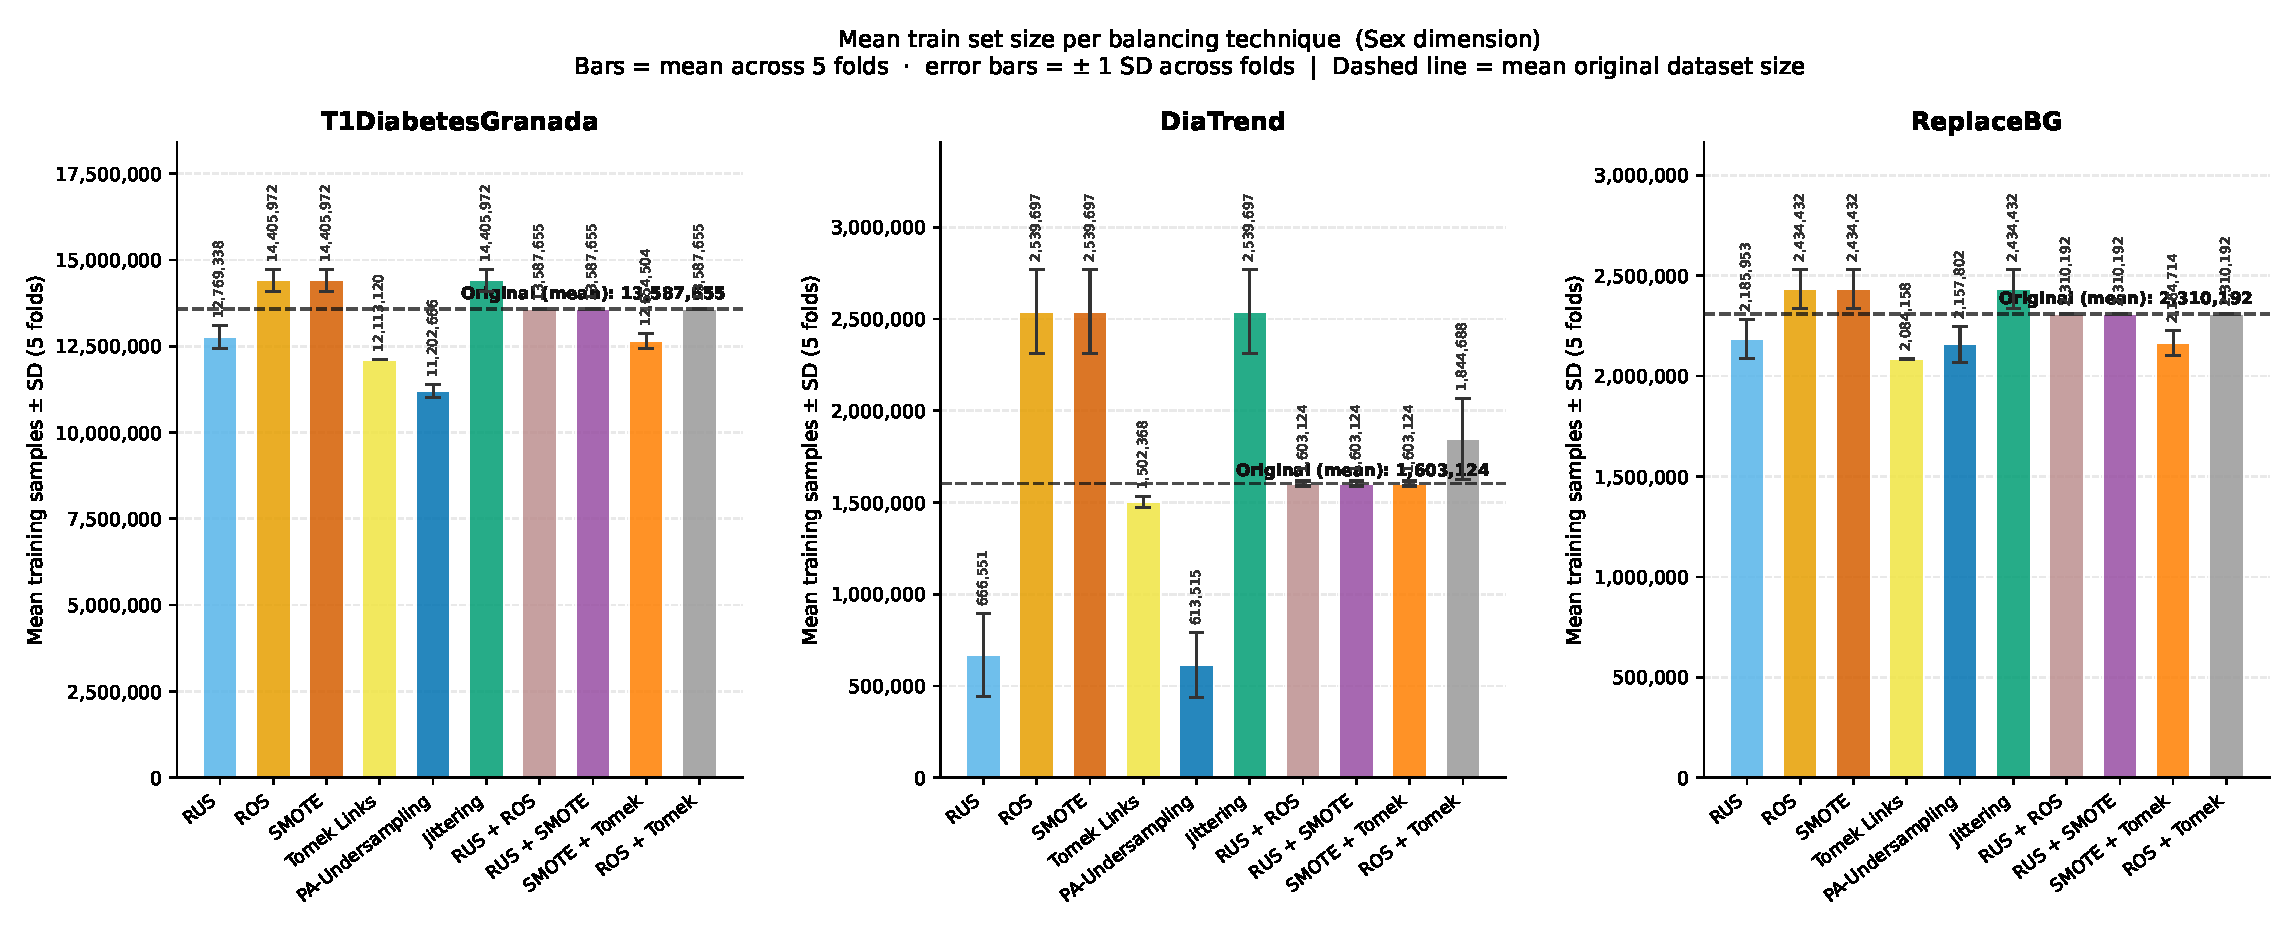
\includegraphics[width=\textwidth]{../../analysis_relief/outputs_clinical/trainsize_bars_sex}
    \caption{Tamaño medio del conjunto de entrenamiento por técnica de balanceo
             y \textit{dataset}, para la dimensión demográfica \textbf{sexo}.
             Misma escala relativa y convenciones que la
             figura~\ref{fig:trainsize_age}.}
    \label{fig:trainsize_sex}
\end{figure}

\paragraph{Implicación metodológica.}
Este análisis tiene una consecuencia directa para la interpretación de los
resultados de predicción. En DiaTrend, las técnicas de aumento por edad
multiplican el volumen de entrenamiento por un factor de hasta 3{,}6$\times$,
mientras que las de reducción lo comprimen al 4\,\% del original. Una mejora
o un deterioro del rendimiento LSTM en este repositorio podría deberse
principalmente al cambio de volumen y no al reequilibrio demográfico en sí.
El caso contrario, REPLACE-BG con la dimensión sexo, ilustra el extremo opuesto:
las variaciones de tamaño son tan pequeñas ($<$6\,\%) que cualquier diferencia
de rendimiento debe atribuirse casi exclusivamente a la redistribución demográfica.
T1DiabetesGranada ocupa una posición intermedia en la dimensión edad pero se
comporta como REPLACE-BG en la dimensión sexo, lo que permite distinguir
empíricamente ambos efectos comparando los resultados de las dos dimensiones
dentro del mismo repositorio. Este contraste estructural es uno de los ejes
interpretativos centrales del análisis de predicción de la
sección~\ref{sec:efecto_balanceo_prediccion}.

% ---------------------------------------------------------
\subsection{Impacto sobre la distribución demográfica del entrenamiento}
\label{subsec:impacto_demografico}
% ---------------------------------------------------------

Los heatmaps de las figuras~\ref{fig:heatmap_age_t1d},
\ref{fig:heatmap_age_diatrend} y~\ref{fig:heatmap_age_replacbg} cuantifican
la variación $\Delta n$ y $\Delta\%$ de ventanas de entrenamiento por grupo
de edad introducida por cada técnica, con escala de color unificada entre los
tres \textit{datasets} para permitir comparación directa. Valores positivos
(naranja) indican incremento de ventanas en ese grupo demográfico; negativos
(morado), reducción. La intensidad del color es proporcional al $\Delta\%$
relativo, de modo que la saturación visual es directamente comparable entre
repositorios.

\begin{figure}[H]
    \centering
    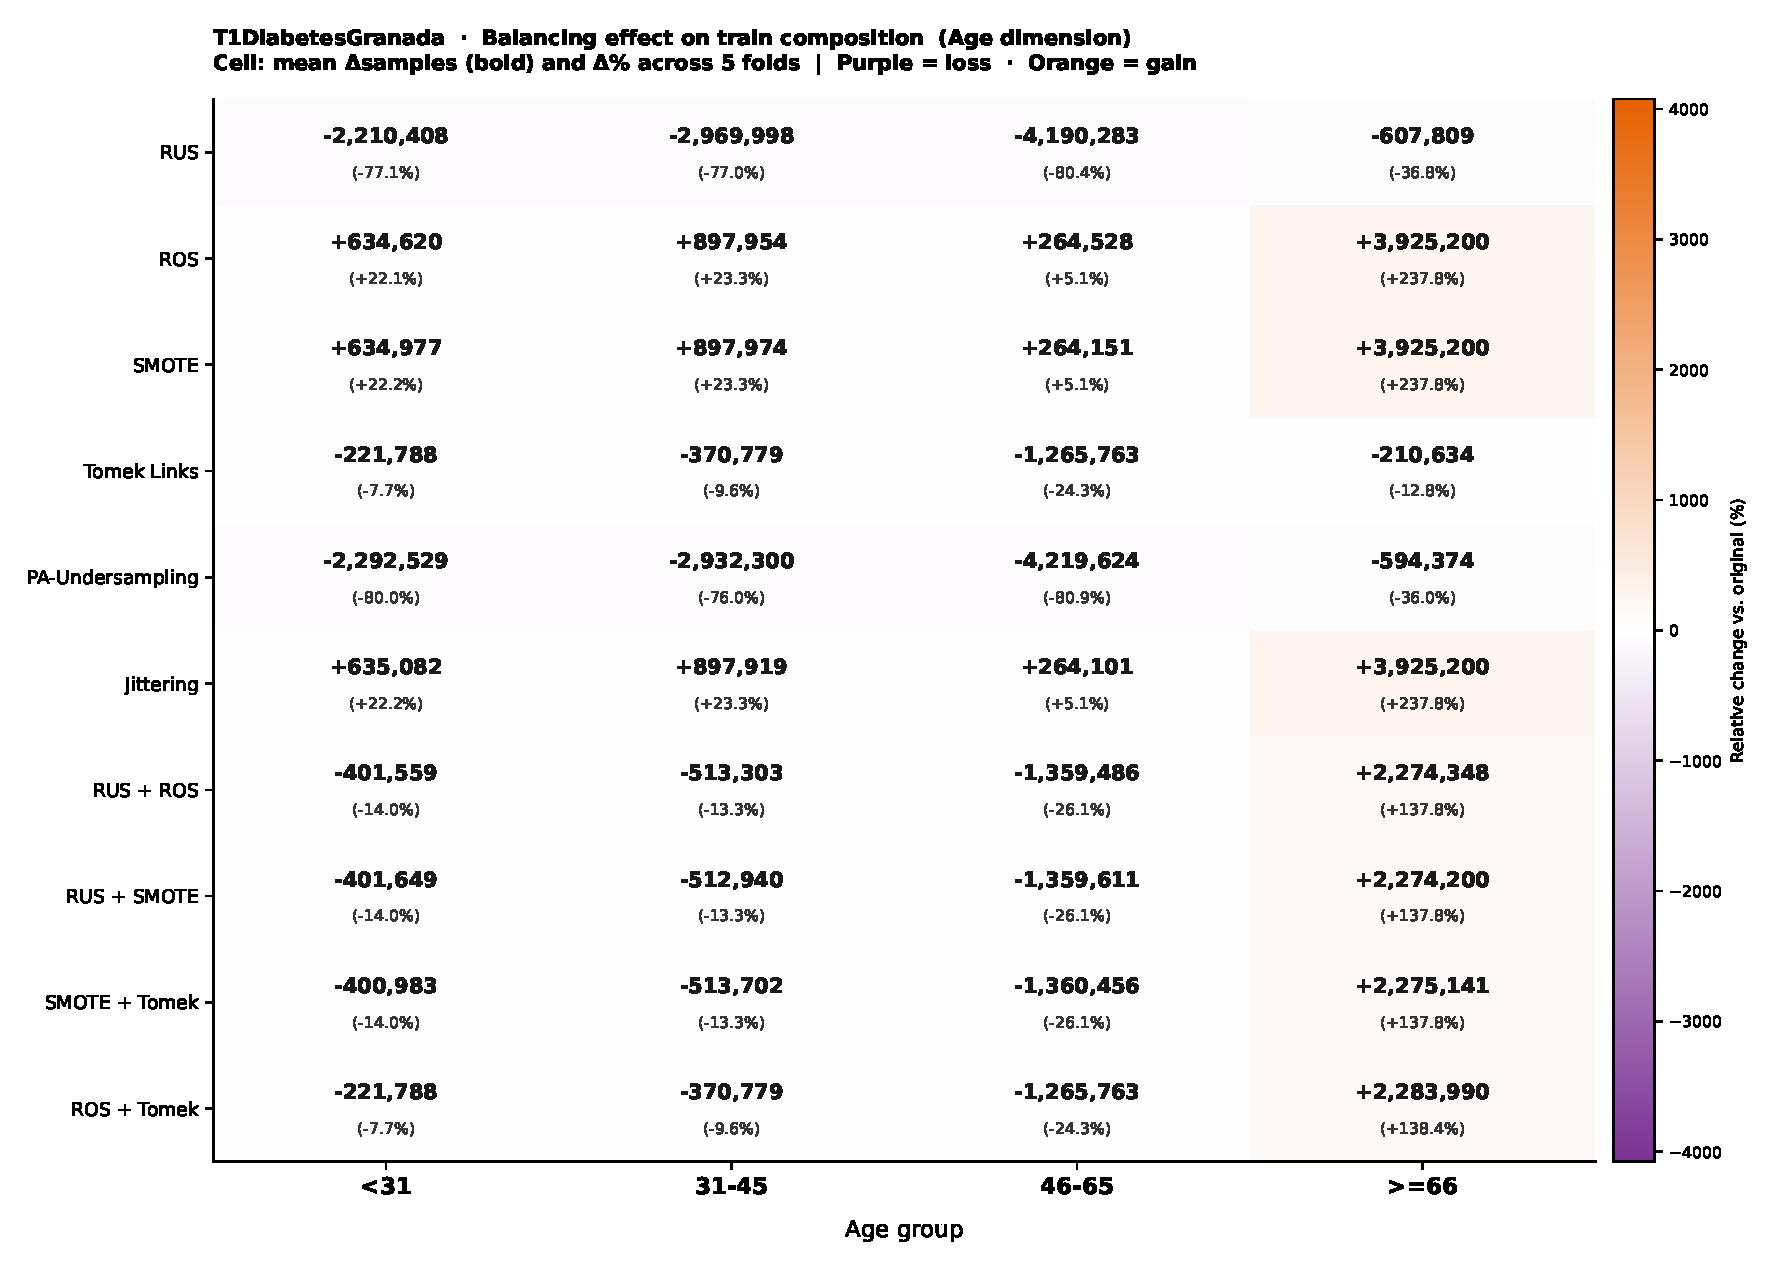
\includegraphics[width=\textwidth]{%
        ../../analysis_relief/outputs_clinical/heatmap_balancing_T1DiabetesGranada_age}
    \caption{Variación $\Delta n$ y $\Delta\%$ de ventanas por técnica de
             balanceo y grupo de edad en \textbf{T1DiabetesGranada}. Escala
             de color unificada con las
             figuras~\ref{fig:heatmap_age_diatrend}
             y~\ref{fig:heatmap_age_replacbg}. Las filas corresponden a las
             diez técnicas evaluadas; las columnas, a los grupos de edad
             ($<$31, 31--45, 46--65, $\geq$66).}
    \label{fig:heatmap_age_t1d}
\end{figure}

En T1DiabetesGranada el desequilibrio de partida es moderado, lo que se
refleja en variaciones $\Delta\%$ contenidas y en una saturación del heatmap
notablemente inferior a la de DiaTrend. Las técnicas de reducción (RUS y
PA-Undersampling) aplican cortes homogéneos entre grupos: RUS elimina
entre el 77 y el 80\,\% de las ventanas en los tres grupos de mediana edad
($<$31: $-77{,}1\%$; 31--45: $-77{,}0\%$; 46--65: $-80{,}4\%$), pero solo
un $-36{,}8\%$ en el grupo $\geq$66, el minoritario. Este comportamiento
asimétrico es precisamente el esperado: al fijar una cuota igual entre grupos,
el grupo con menos ventanas sufre una reducción proporcionalmente menor.
PA-Undersampling reproduce un patrón casi idéntico al de RUS ($-80{,}0\%$,
$-76{,}0\%$, $-80{,}9\%$, $-36{,}0\%$), lo que indica que en un dataset
con seguimientos tan heterogéneos como T1DiabetesGranada la cuota por
paciente no introduce diferencias relevantes respecto al submuestreo puramente
aleatorio.

Las técnicas de aumento (ROS, SMOTE, Jittering) concentran el incremento en
el grupo $\geq$66: las tres añaden $+3\,925\,200$ ventanas a ese grupo
($+237{,}8\%$), mientras que el incremento en los grupos $<$31 y 31--45 es
moderado ($\approx+22\%$ y $+23\%$) y en 46--65 es casi nulo ($+5{,}1\%$),
reflejo de que ese grupo ya es el más numeroso y requiere poco o ningún
aumento para igualarse a la cuota objetivo. Tomek Links produce reducciones
pequeñas pero no uniformes: elimina el 24{,}3\,\% de las ventanas del grupo
46--65 (el más numeroso y por tanto el más afectado por la limpieza de
frontera) frente a solo el 7--10\,\% en los grupos menores.

Las técnicas híbridas muestran el patrón de compensación esperado: RUS+ROS,
RUS+SMOTE y SMOTE+Tomek reducen los tres grupos mayoritarios
($-14\%$, $-13\%$, $-26\%$ en $<$31, 31--45 y 46--65) e incrementan
sustancialmente el $\geq$66 ($+137{,}8\%$), logrando la redistribución más
equilibrada de todas las familias sin modificar el tamaño total del train.
ROS+Tomek produce un perfil similar pero con reducciones algo más contenidas
gracias a que el Tomek posterior modera el sobreajuste del ROS previo.

\begin{figure}[H]
    \centering
    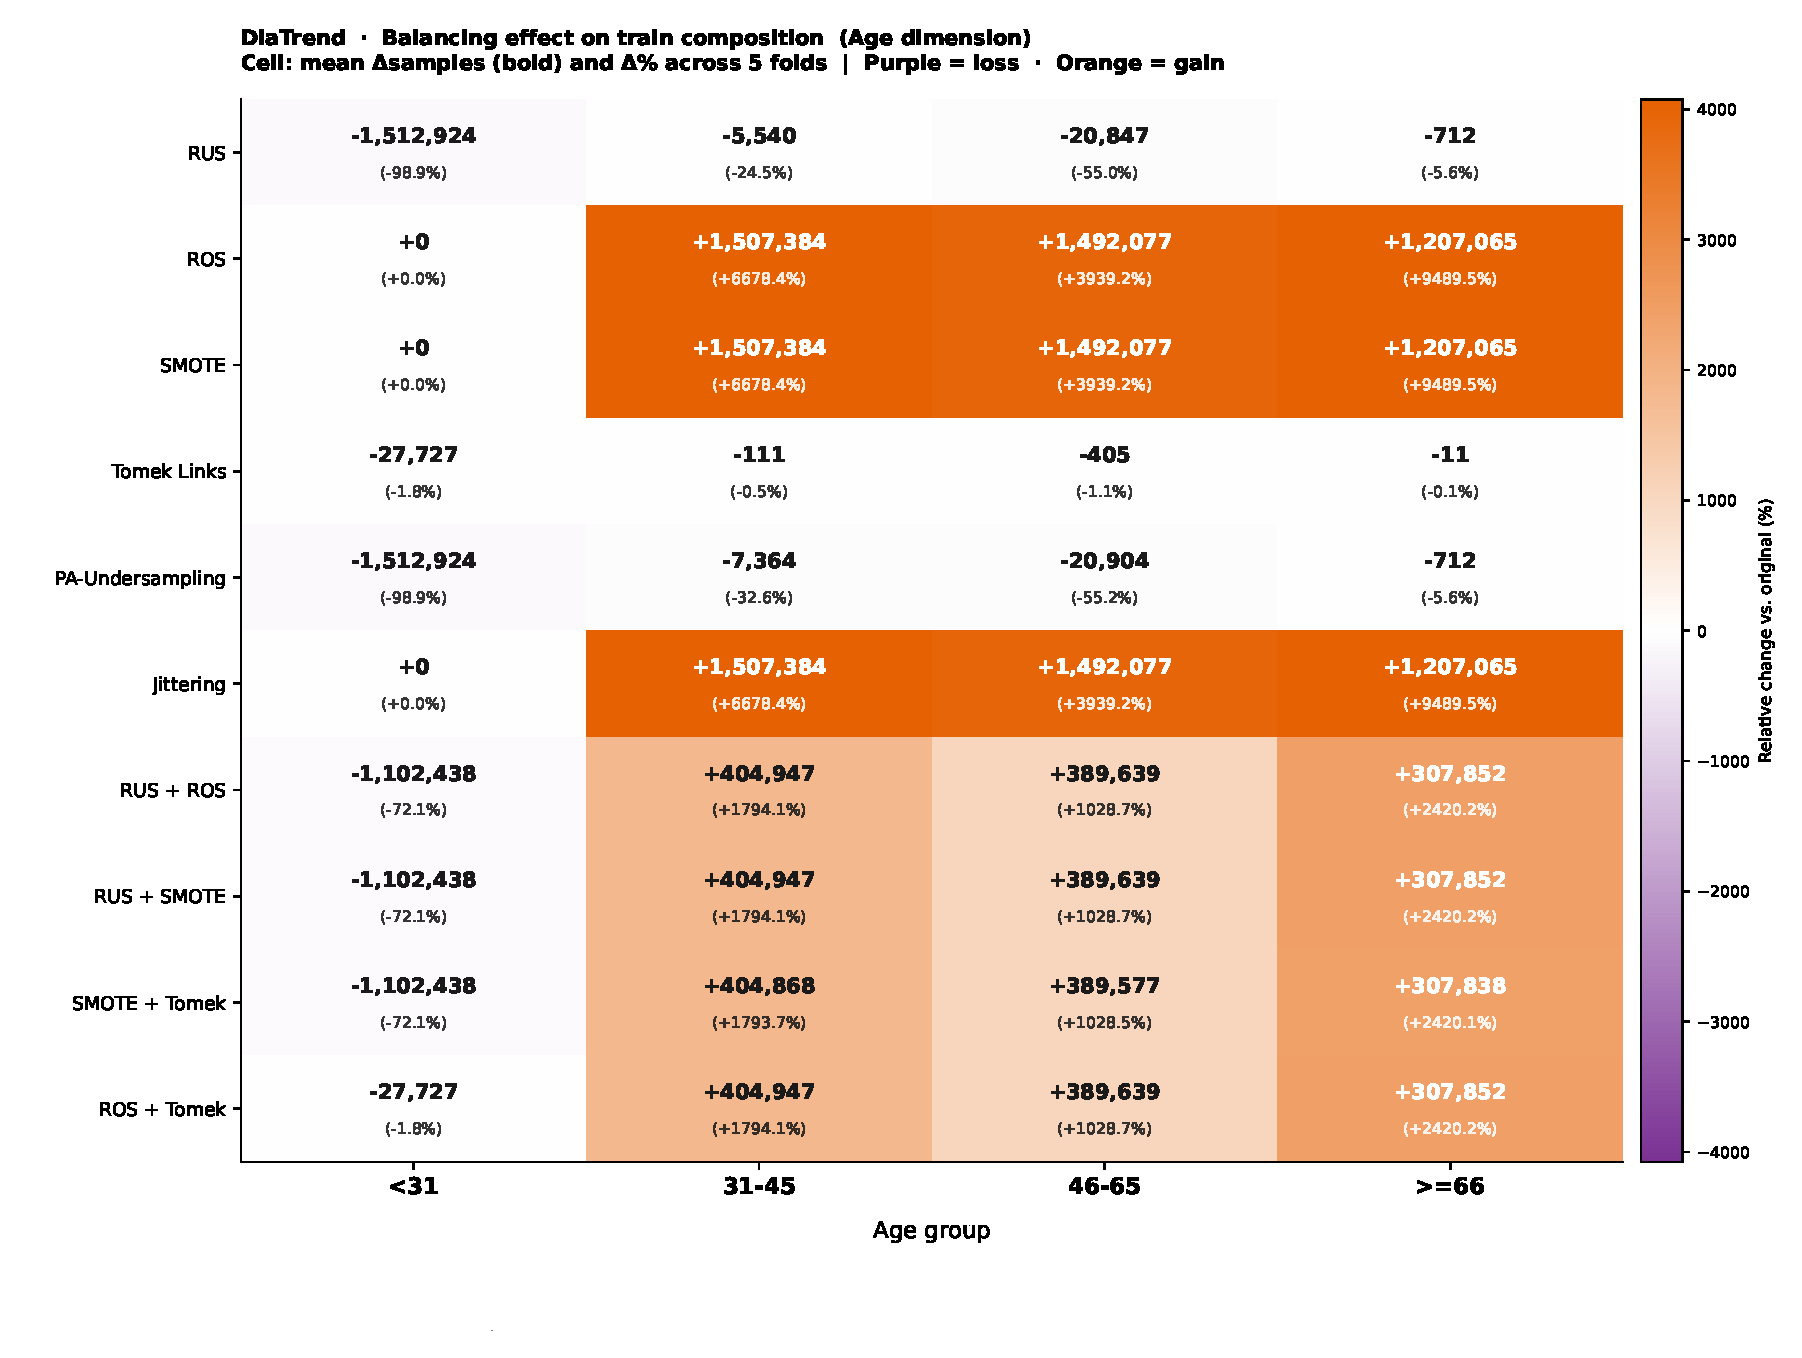
\includegraphics[width=\textwidth]{%
        ../../analysis_relief/outputs_clinical/heatmap_balancing_DIATREND_age}
    \caption{Variación $\Delta n$ y $\Delta\%$ de ventanas por técnica de
             balanceo y grupo de edad en \textbf{DiaTrend}. La escala de
             color es la misma que en la figura~\ref{fig:heatmap_age_t1d};
             la saturación visiblemente superior en este \textit{dataset}
             refleja el desequilibrio demográfico extremo documentado en la
             sección~\ref{subsec:eda_demografico}.}
    \label{fig:heatmap_age_diatrend}
\end{figure}

En DiaTrend el impacto del balanceo sobre la distribución demográfica es
cualitativamente diferente al de T1DiabetesGranada: incluso a escala unificada,
el heatmap aparece prácticamente saturado en naranja para las técnicas de
aumento, lo que indica variaciones relativas de un orden de magnitud superior.
La causa es el desequilibrio extremo del repositorio: el grupo $<$31 concentra
el 97\,\% de las ventanas originales, mientras que los grupos 31--45, 46--65 y
$\geq$66 apenas aportan el 3\,\% restante.

Las técnicas de reducción (RUS, PA-Undersampling) eliminan el
98{,}9\,\% de las ventanas del grupo $<$31, reduciéndolo de más de
1{,}5 millones a apenas 63\,100 y 61\,220 respectivamente. Los grupos
minoritarios también se reducen, pero en mucha menor proporción ($-24{,}5\%$
en 31--45 para RUS, $-55{,}0\%$ en 46--65, $-5{,}6\%$ en $\geq$66),
con el resultado de que el train resultante contiene un número de ventanas
tan pequeño que compromete la capacidad de generalización del modelo.

Las técnicas de aumento (ROS, SMOTE, Jittering) mantienen inalterado el
grupo $<$31 (ya mayoritario, $\Delta n = 0$) y multiplican los grupos
minoritarios por factores extremos: $+6\,678\%$ en 31--45,
$+3\,939\%$ en 46--65 y $+9\,490\%$ en $\geq$66. En términos absolutos,
el grupo $\geq$66 ---un único paciente con 12\,732 ventanas originales---
recibe más de 1{,}2 millones de ventanas sintéticas o duplicadas, lo que
equivale a replicar ese único perfil glucémico casi 95 veces. Esta
estrategia consigue el reequilibrio numérico requerido, pero introduce
una forma severa de redundancia que puede inducir sobreajuste y reduce
drásticamente la diversidad efectiva del entrenamiento para ese grupo.

Las técnicas híbridas (RUS+ROS, RUS+SMOTE, SMOTE+Tomek) reducen el grupo
$<$31 en un $-72{,}1\%$ y compensan con incrementos de $+1\,794\%$,
$+1\,029\%$ y $+2\,420\%$ en los grupos 31--45, 46--65 y $\geq$66
respectivamente. ROS+Tomek, al no aplicar submuestreo previo, mantiene
el grupo $<$31 reducido solo un $-1{,}8\%$ (efecto Tomek puro) y aplica
los mismos incrementos sobre los grupos minoritarios que las híbridas
completas, ocupando así una posición intermedia entre aumento puro e
híbrida compensada.

\begin{figure}[H]
    \centering
    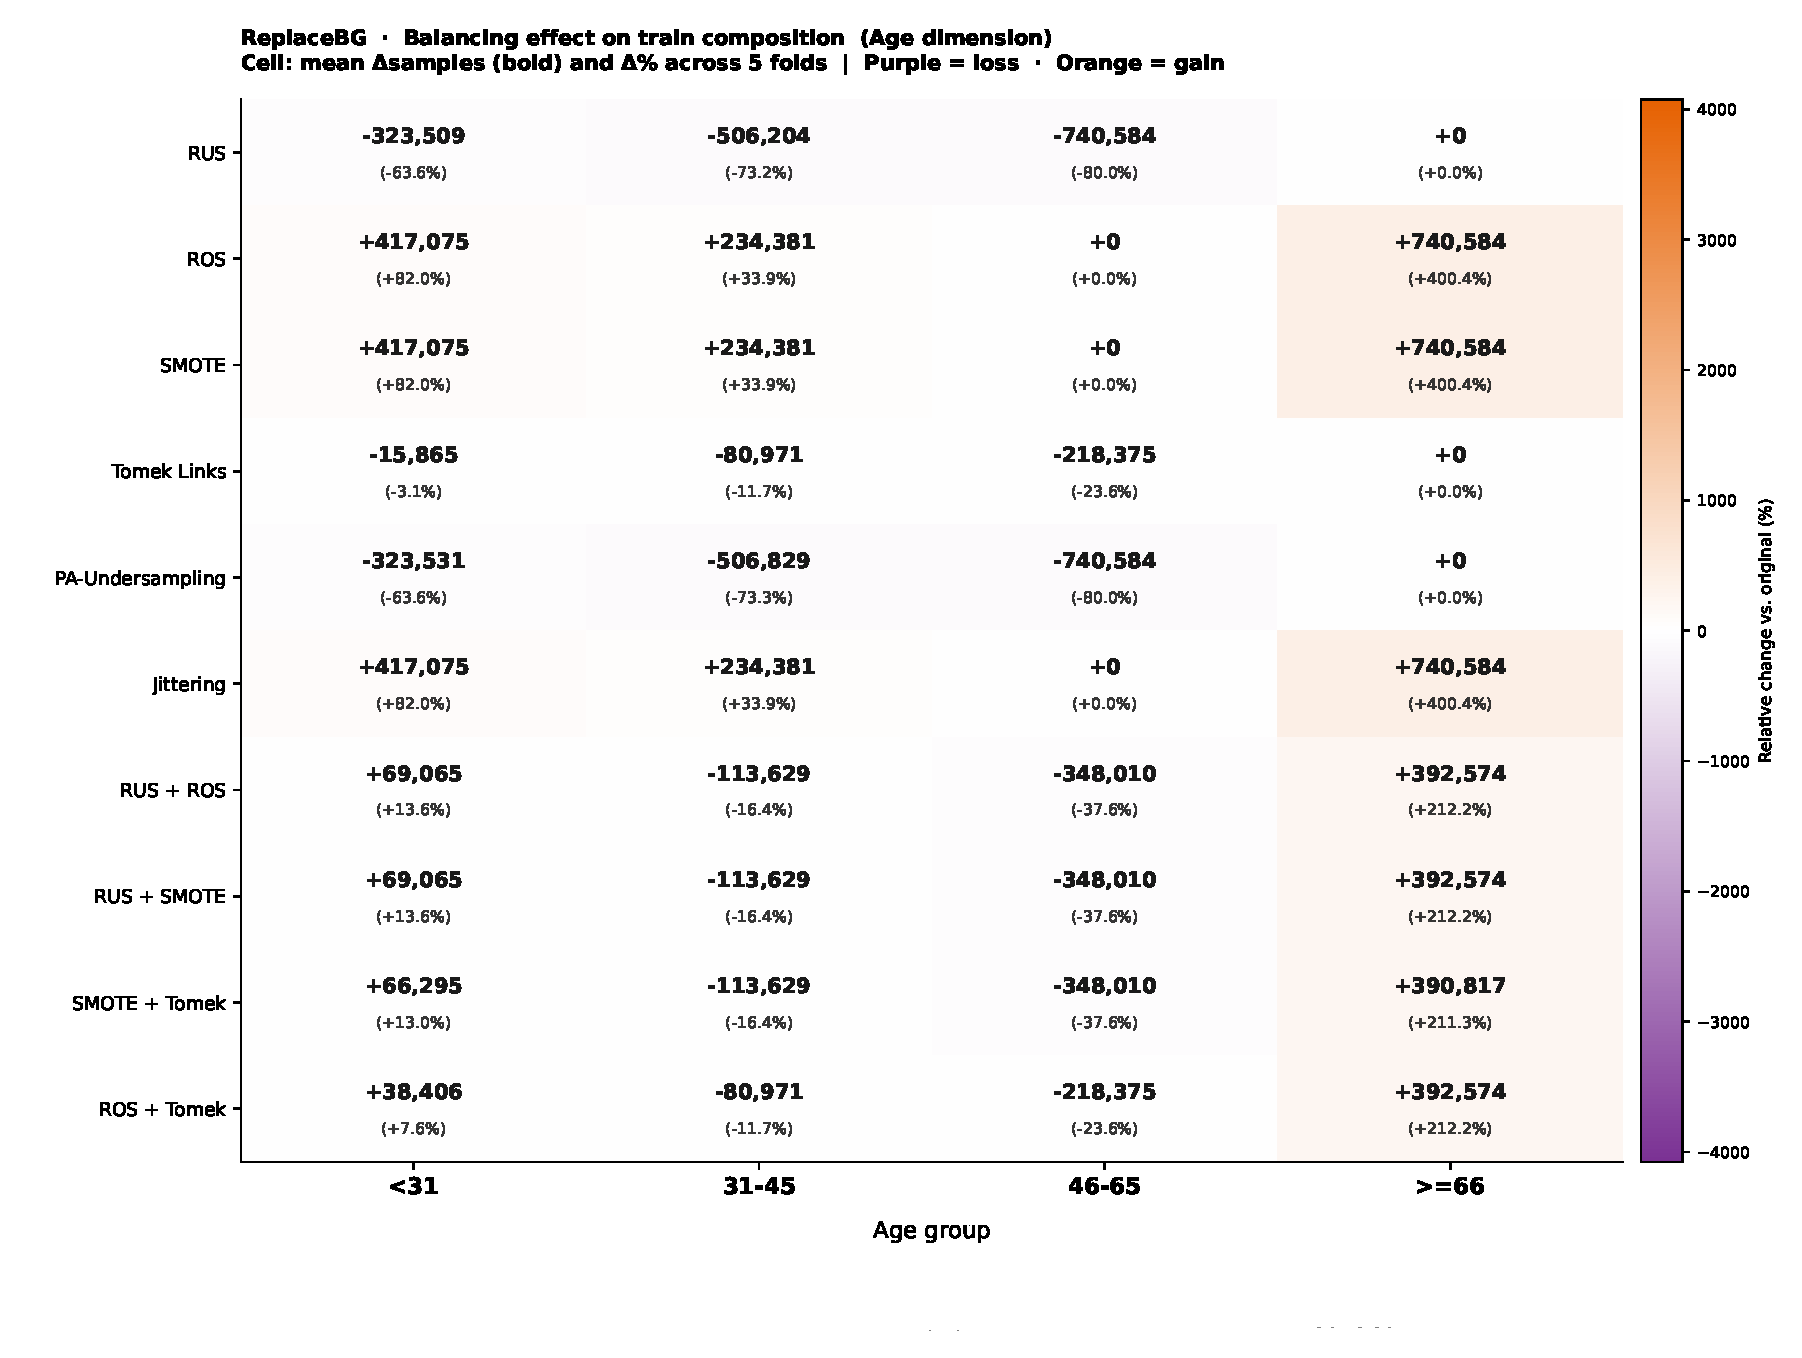
\includegraphics[width=\textwidth]{%
        ../../analysis_relief/outputs_clinical/heatmap_balancing_REPLACE-BG_age}
    \caption{Variación $\Delta n$ y $\Delta\%$ de ventanas por técnica de
             balanceo y grupo de edad en \textbf{REPLACE-BG}. La menor
             saturación respecto a DiaTrend (figura~\ref{fig:heatmap_age_diatrend}),
             con escala idéntica, confirma que el diseño controlado del estudio
             ---con seguimientos homogéneos de $\approx$182 días para todos
             los grupos--- limita la amplificación del desequilibrio demográfico
             al pasar de paciente a ventana.}
    \label{fig:heatmap_age_replacbg}
\end{figure}

REPLACE-BG presenta un patrón intermedio entre los dos anteriores: el
desequilibrio de partida es real (el grupo 46--65 es el más numeroso y el
$\geq$66 el más pequeño), pero la homogeneidad de los seguimientos impide
que ese desequilibrio demográfico se amplifique al nivel de ventana de la
forma extrema observada en DiaTrend.

Las técnicas de reducción eliminan en mayor proporción los grupos intermedios
y mayoritarios: RUS recorta el 46--65 en un $-80\%$ ($-740\,584$ ventanas),
el 31--45 en un $-73{,}2\%$ y el $<$31 en un $-63{,}6\%$, pero deja
inalterado el grupo $\geq$66 (que ya es el minoritario y define la cuota
objetivo). PA-Undersampling reproduce casi exactamente el mismo patrón.
Tomek Links aplica reducciones más contenidas y concentradas en el grupo
mayoritario ($-23{,}6\%$ en 46--65, $-11{,}7\%$ en 31--45, $-3{,}1\%$
en $<$31), sin afectar al $\geq$66.

Las técnicas de aumento siguen la lógica inversa: ROS, SMOTE y Jittering
incrementan el $\geq$66 en un $+400{,}4\%$ ($+740\,584$ ventanas) y el
$<$31 en un $+82\%$ ($+417\,075$), mientras dejan el 31--45 con un aumento
moderado ($+33{,}9\%$) y el 46--65 sin cambio ($\Delta n = 0$, pues es el
grupo de referencia que marca la cuota). Este patrón difiere del observado
en T1DiabetesGranada, donde la asimetría se concentraba exclusivamente en
el $\geq$66: en REPLACE-BG los grupos $<$31 y $\geq$66 comparten el papel
de grupos infrarrepresentados, lo que distribuye el esfuerzo de aumento
entre ambos extremos etarios.

Las técnicas híbridas presentan el patrón de compensación más claro de los
tres repositorios: RUS+ROS y RUS+SMOTE reducen los grupos 31--45 ($-16{,}4\%$)
y 46--65 ($-37{,}6\%$) e incrementan simultáneamente $<$31 ($+13{,}6\%$) y
$\geq$66 ($+212{,}2\%$), con celdas azules y naranjas alternadas que reflejan
la compensación cruzada entre submuestreo y sobremuestreo.

En conjunto, los tres heatmaps confirman que el balanceo demográfico modifica
la composición del conjunto de entrenamiento de forma significativa en todos
los \textit{datasets}, pero la magnitud y el patrón del cambio son
fuertemente dependientes del repositorio: desde variaciones del orden del
$\pm$25\% en T1DiabetesGranada hasta multiplicaciones por factores de
$\times$95 en el grupo $\geq$66 de DiaTrend. La siguiente subsección analiza
si estas modificaciones tienen un correlato en la distribución glucémica del
entrenamiento, que es la dimensión directamente relevante para el rendimiento
clínico del modelo.




% ---------------------------------------------------------
\subsection{Impacto sobre la distribución glucémica del entrenamiento}
\label{subsec:impacto_glucemico}
% ---------------------------------------------------------

La redistribución demográfica descrita en la subsección anterior no opera
directamente sobre las métricas de predicción: lo que el modelo LSTM aprende
es la distribución de valores glucémicos en el entrenamiento, no las etiquetas
demográficas de los pacientes. El mecanismo por el que el balanceo demográfico
puede influir en el rendimiento clínico es, por tanto, indirecto: al modificar
la composición por grupos de edad o sexo, se altera implícitamente la
proporción de ventanas en cada rango glucémico (TBR-2, TBR-1, TIR, TAR-1,
TAR-2), porque los distintos subgrupos demográficos presentan perfiles
glucémicos diferentes (véase sección~\ref{subsec:eda_cgm}). Esta subsección
cuantifica ese efecto indirecto.

Las figuras de barras apiladas muestran la composición absoluta del conjunto
de entrenamiento por rango glucémico; las figuras de barras divergentes
muestran la variación $\Delta\%$ respecto al conjunto original, que es la
lectura clínicamente relevante: un incremento en TBR-2 indica que el modelo
recibirá más ejemplos de hipoglucemia severa, con el potencial de mejorar
su sensibilidad a esos eventos.

\paragraph{T1DiabetesGranada.}

\begin{figure}[H]
    \centering
    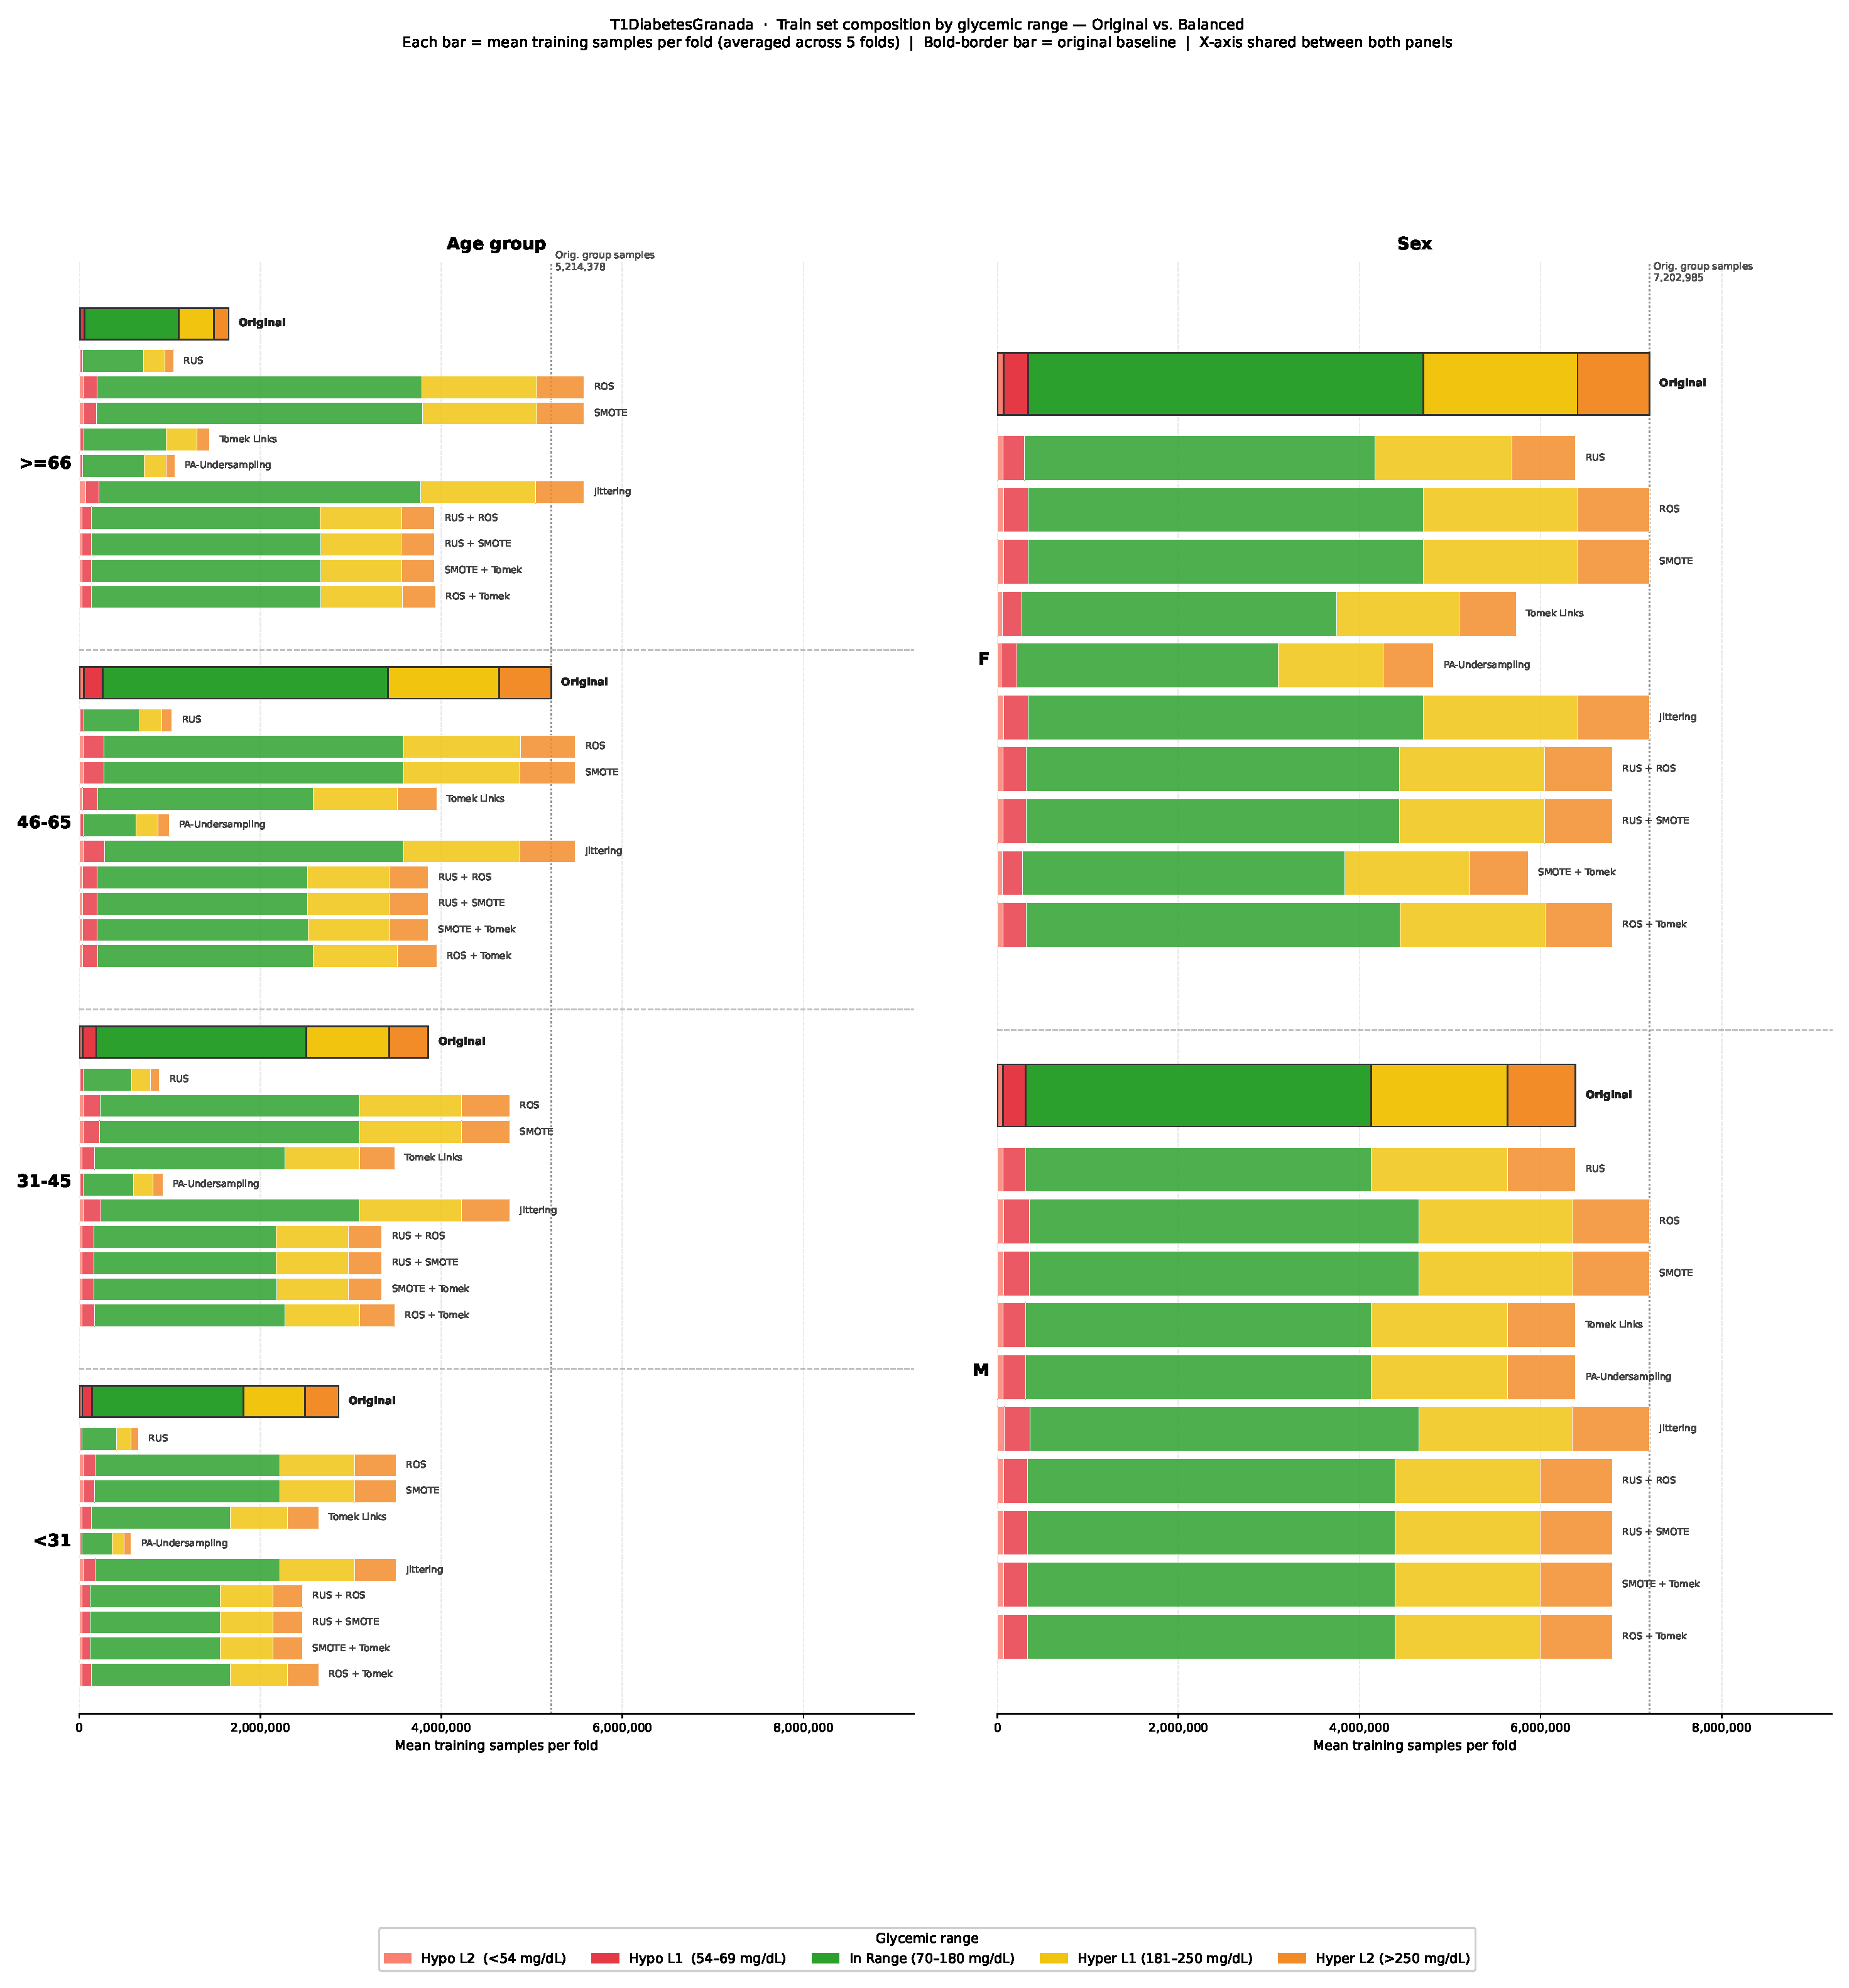
\includegraphics[width=\textwidth]{%
        ../../analysis_relief/outputs_clinical/stacked_bars_T1DiabetesGranada}
    \caption{Distribución de ventanas por rango glucémico en el conjunto de
             entrenamiento de \textbf{T1DiabetesGranada}, por técnica de
             balanceo y dimensión demográfica. Cada barra representa la media
             sobre los 5 \textit{folds}. La barra con borde grueso es la
             condición original de referencia.}
    \label{fig:stacked_t1d}
\end{figure}

En T1DiabetesGranada la distribución glucémica del conjunto original está
ampliamente dominada por la normoglucemia (TIR, franja verde), que supera
los 5{,}2 millones de ventanas por \textit{fold} en la dimensión edad frente
a contribuciones mucho menores de los rangos extremos. Las técnicas de
reducción (RUS, PA-Undersampling) comprimen toda la distribución de forma
aproximadamente proporcional, por lo que la composición relativa por rangos
apenas varía visualmente respecto al original. Las técnicas de aumento
(ROS, SMOTE, Jittering) amplían principalmente el grupo $\geq$66, que como
se mostró en la sección~\ref{subsec:impacto_demografico} es el más
infrarrepresentado; dado que ese grupo presenta un perfil glucémico con mayor
proporción de TIR y menor de TAR (véase sección~\ref{subsec:eda_cgm}), su
amplificación se traduce en un ligero desplazamiento de la distribución
hacia la normoglucemia.

\begin{figure}[H]
    \centering
    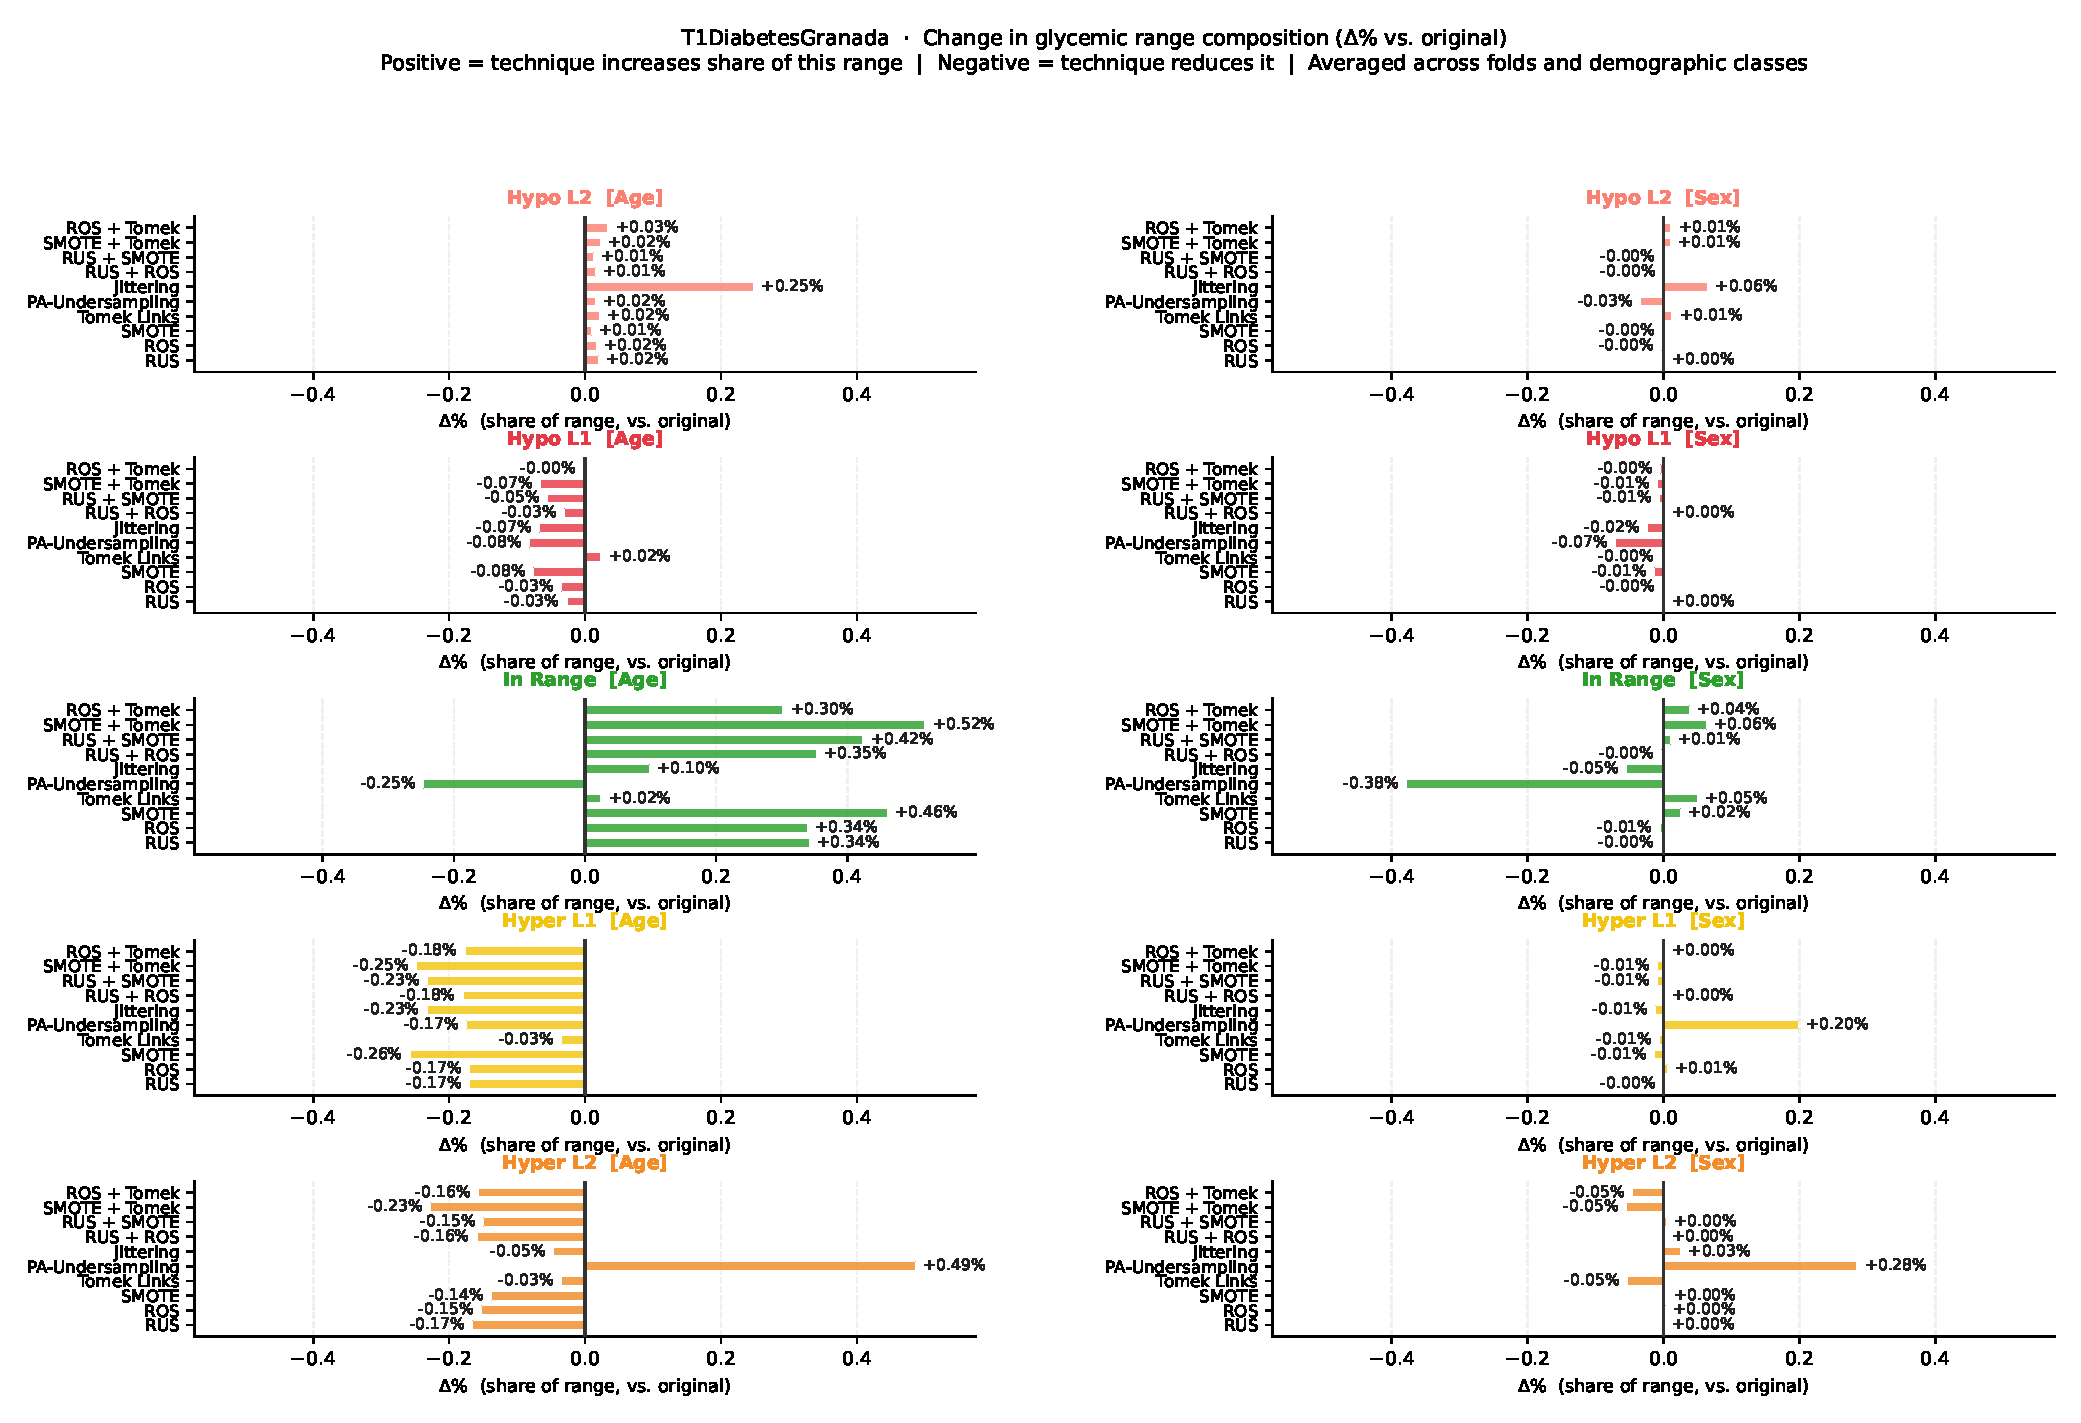
\includegraphics[width=\textwidth]{%
        ../../analysis_relief/outputs_clinical/delta_glycemic_T1DiabetesGranada}
    \caption{Variación $\Delta\%$ en la representación de cada rango glucémico
             para \textbf{T1DiabetesGranada} tras aplicar cada técnica, respecto
             al conjunto original. Barras divergentes: positivo = mayor
             representación del rango; negativo = menor. Promediado sobre
             \textit{folds} y clases demográficas.}
    \label{fig:delta_glycemic_t1d}
\end{figure}

Las barras divergentes de la figura~\ref{fig:delta_glycemic_t1d} confirman
que los cambios en la composición glucémica son de magnitud muy pequeña en
todos los rangos y técnicas. En la dimensión edad, los cambios más destacables
son: Jittering incrementa TBR-2 en $+0{,}25\%$ y PA-Undersampling lo reduce
en $-0{,}25\%$ mientras incrementa TIR en $+1{,}15\%$ --- el mayor cambio
individual observado en este dataset, que refleja que PA-Undersampling amplifica
relativamente los grupos con mejor control glucémico medio. SMOTE produce el
mayor desplazamiento hacia TIR ($+0{,}46\%$) y la mayor reducción de TAR-1
($-0{,}26\%$) y TAR-2 ($-0{,}14\%$) entre las técnicas de aumento, mientras
que Tomek Links prácticamente no altera la composición glucémica ($|\Delta\%|
< 0{,}05\%$ en todos los rangos). En la dimensión sexo los cambios son aún
más pequeños, con valores máximos inferiores a $\pm 0{,}44\%$, lo que es
coherente con la menor diferencia glucémica entre sexos documentada en el EDA.

En conjunto, T1DiabetesGranada presenta el escenario en que el balanceo
demográfico tiene el menor impacto glucémico relativo: los cambios son
estadísticamente detectables pero clínicamente marginales, lo que sugiere
que cualquier efecto sobre el rendimiento del modelo en este dataset deberá
atribuirse principalmente al cambio de tamaño del train y no a una
reorientación sustancial de la distribución glucémica de aprendizaje.

\paragraph{DiaTrend.}

\begin{figure}[H]
    \centering
    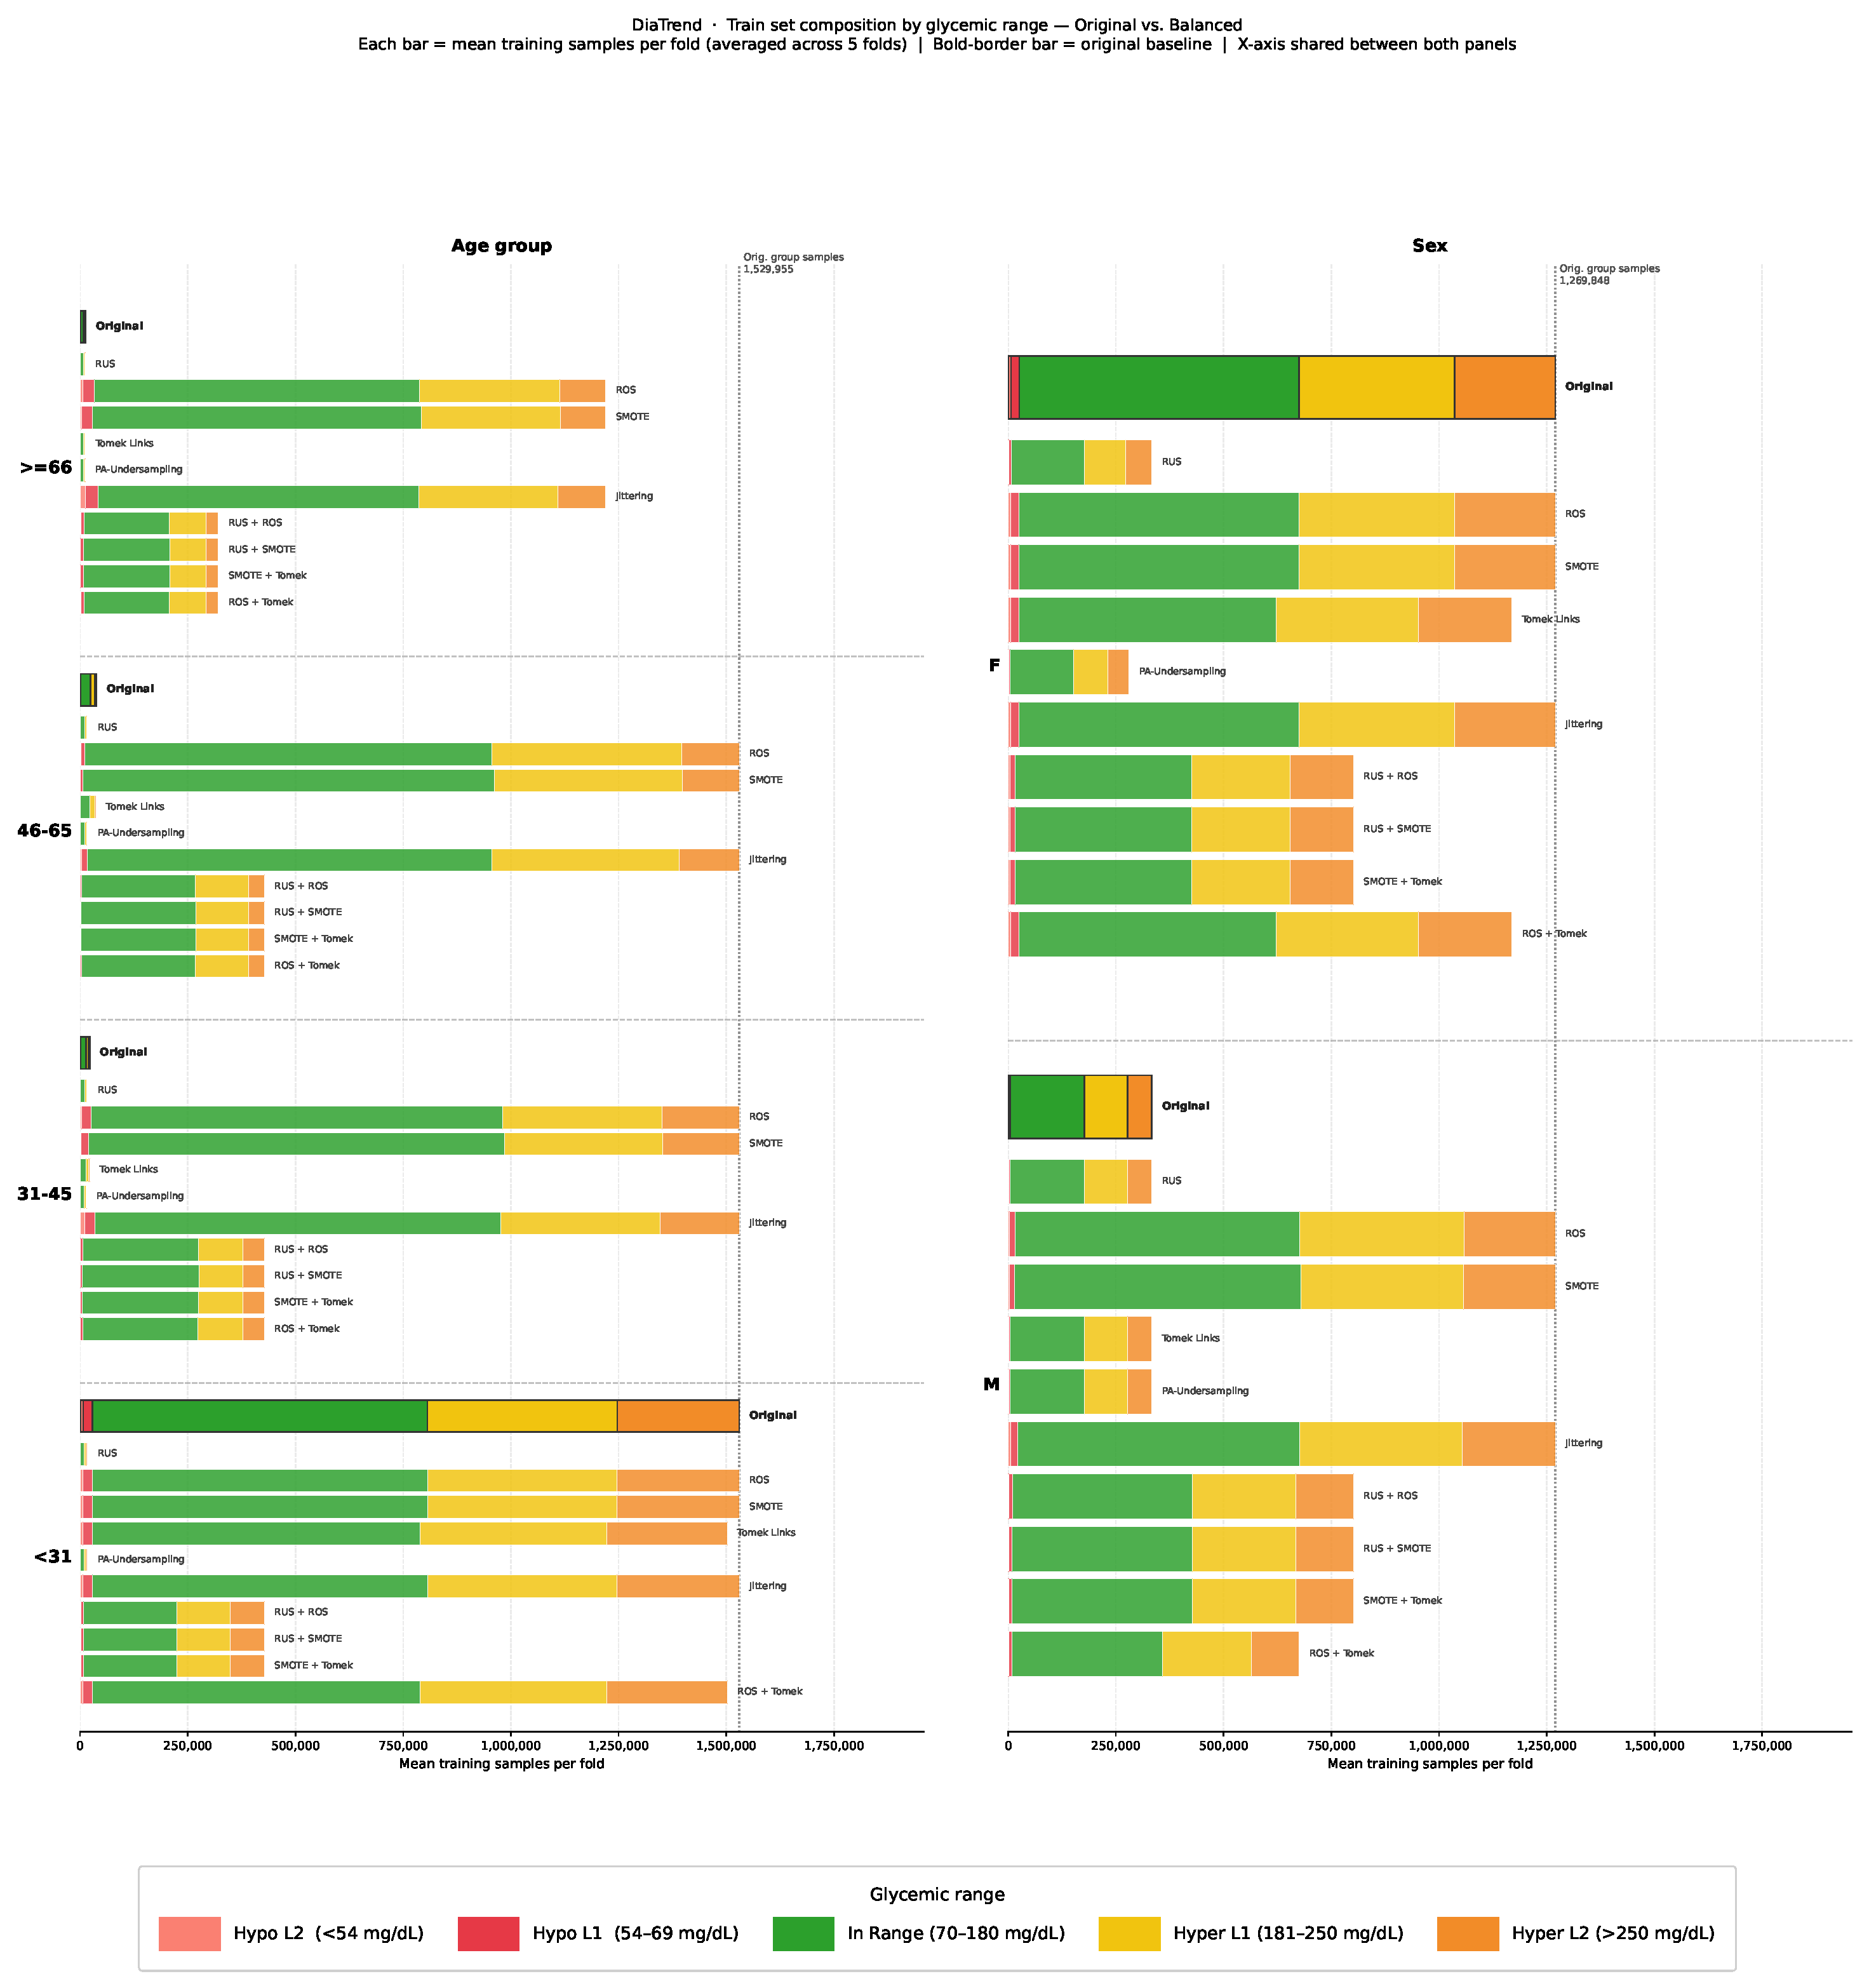
\includegraphics[width=\textwidth]{%
        ../../analysis_relief/outputs_clinical/stacked_bars_DIATREND}
    \caption{Distribución glucémica del conjunto de entrenamiento de
             \textbf{DiaTrend} por técnica y dimensión. Las barras de ROS,
             SMOTE y Jittering alcanzan valores absolutos muy superiores al
             resto como consecuencia del ratio de desequilibrio extremo de
             este \textit{dataset}.}
    \label{fig:stacked_diatrend}
\end{figure}

En DiaTrend la distribución original está igualmente dominada por el TIR,
pero con un volumen absoluto de $\approx$1{,}53 millones de ventanas por
\textit{fold} en el grupo $<$31 (dimensión edad) frente a contribuciones
mínimas de los grupos restantes. Las técnicas de aumento multiplican este
volumen total por un factor de $\approx$3{,}6$\times$ como se documentó en
la sección~\ref{subsec:impacto_tamaño}, y las barras apiladas revelan que
ese incremento se concentra mayoritariamente en el TIR de los grupos
minoritarios: al replicar o sintetizar ventanas del grupo $\geq$66 casi 95
veces, el grueso de las ventanas añadidas son ventanas en normoglucemia,
porque el único paciente de ese grupo tiene un perfil predominantemente
en TIR.

\begin{figure}[H]
    \centering
    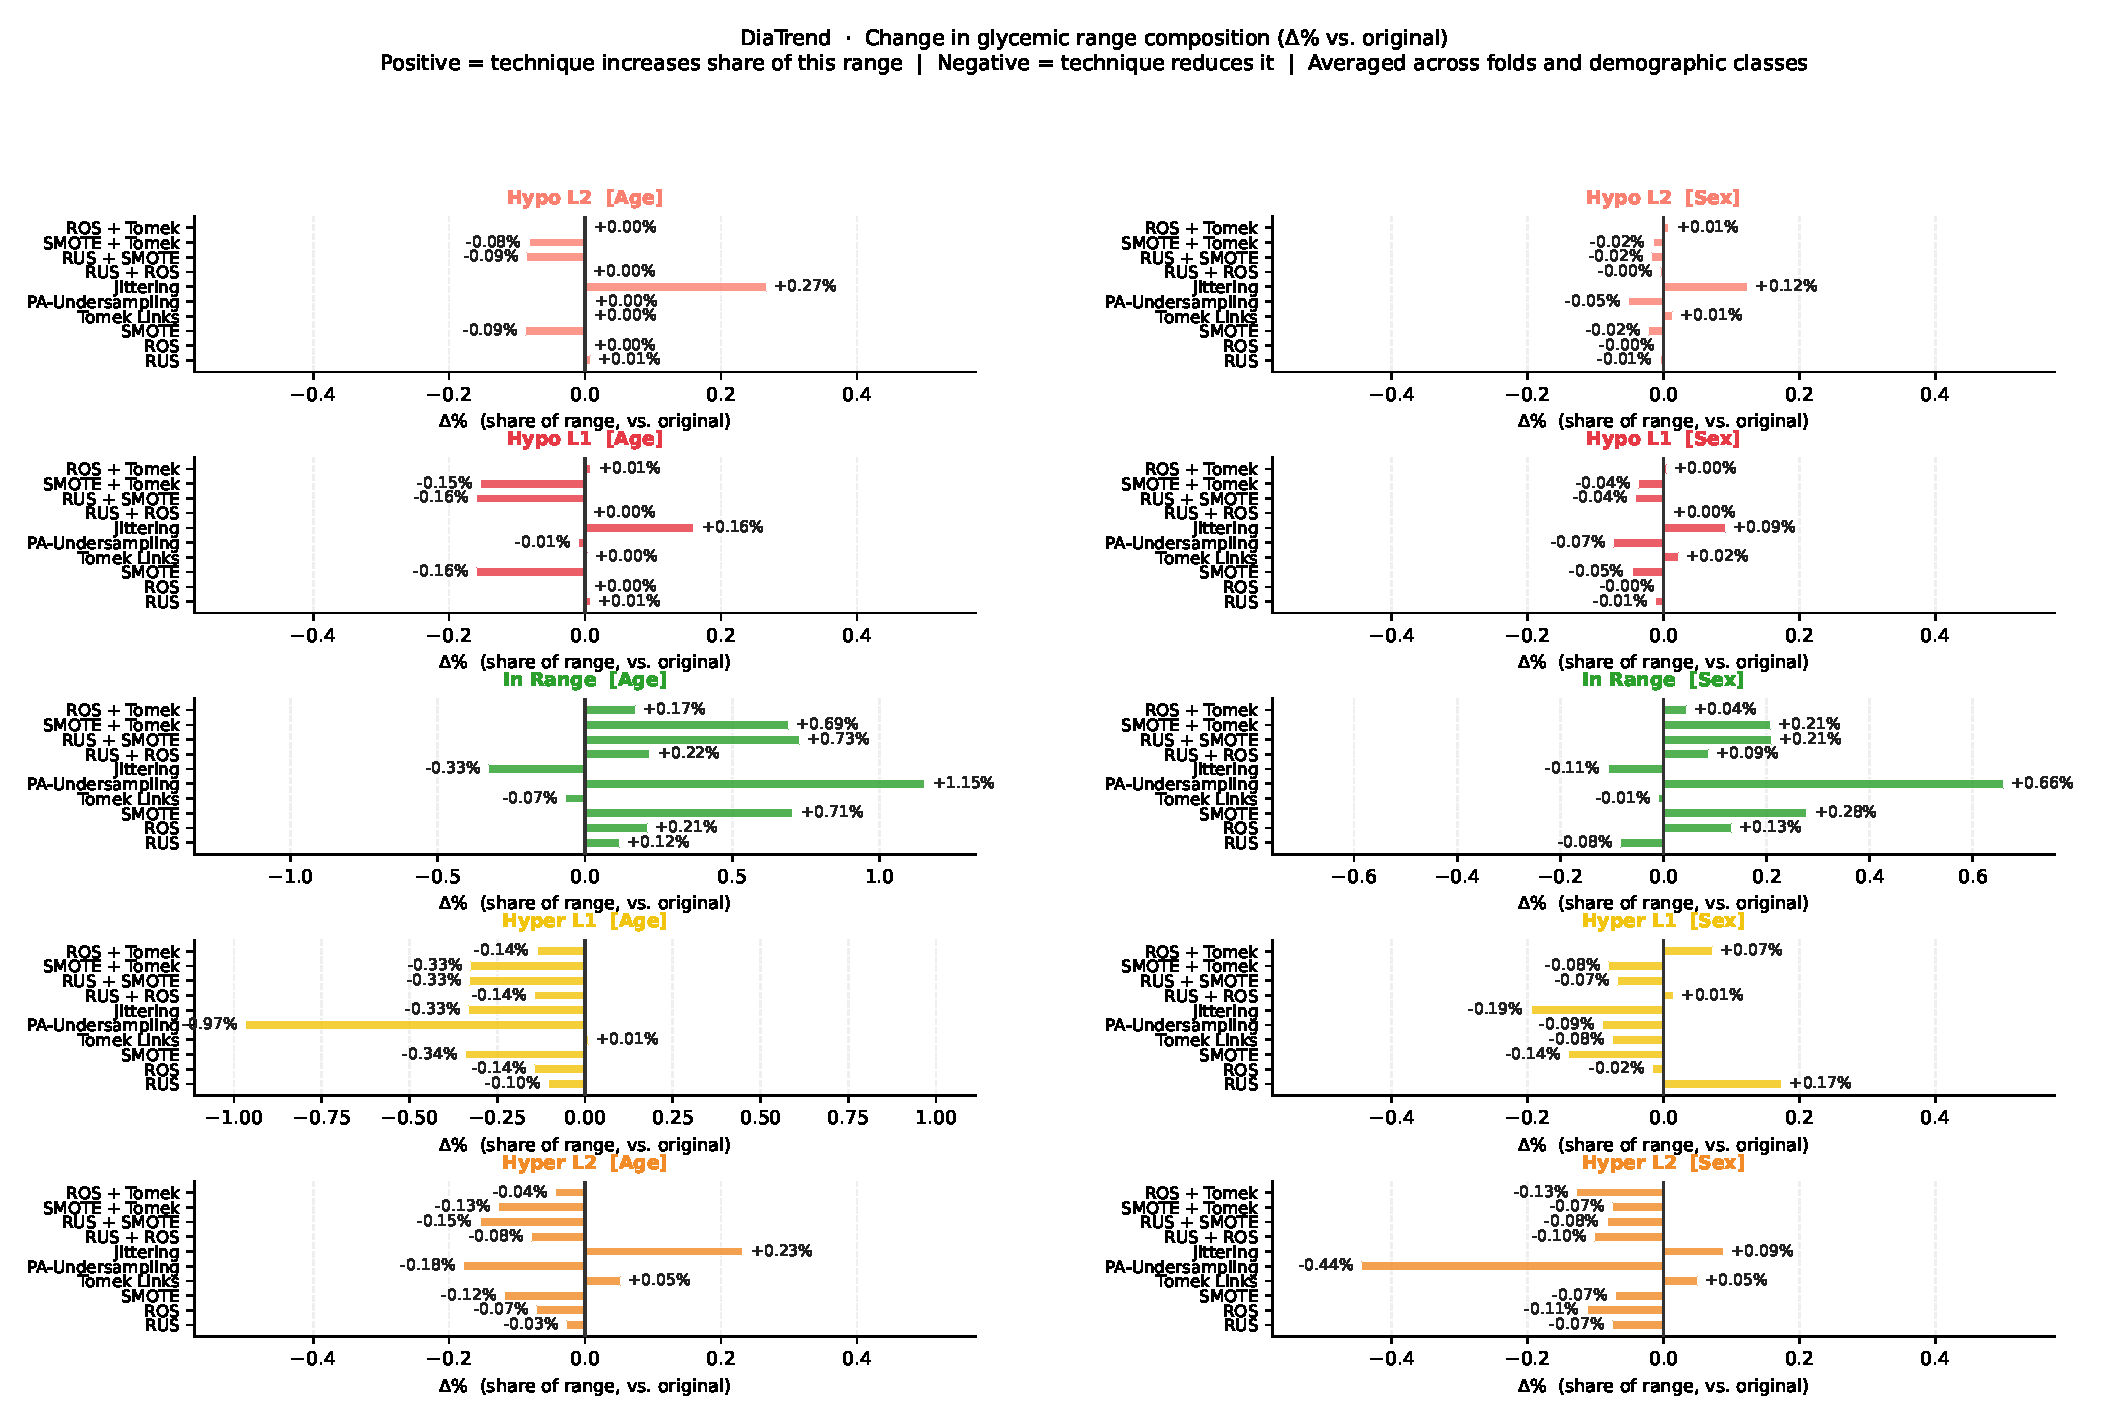
\includegraphics[width=\textwidth]{%
        ../../analysis_relief/outputs_clinical/delta_glycemic_DIATREND}
    \caption{Variación $\Delta\%$ en la representación de rangos glucémicos
             para \textbf{DiaTrend}. La escala del eje es comparable a la
             de T1DiabetesGranada y REPLACE-BG; la magnitud de los cambios
             es notablemente superior en este \textit{dataset}.}
    \label{fig:delta_glycemic_diatrend}
\end{figure}

Las barras divergentes de la figura~\ref{fig:delta_glycemic_diatrend}
muestran los cambios glucémicos más intensos de los tres repositorios.
En la dimensión edad, Jittering produce el mayor incremento de TBR-2
($+0{,}27\%$) y de TIR ($+0{,}33\%$) simultáneamente, mientras reduce
TAR-1 ($-0{,}33\%$) y TAR-2 ($-0{,}23\%$); este patrón es consistente
con amplificar un grupo $\geq$66 con mejor control glucémico relativo.
PA-Undersampling presenta el comportamiento opuesto: incrementa TIR en
$+1{,}15\%$ --- el mayor valor positivo de TIR observado en cualquier
técnica y dataset --- mientras reduce TAR-1 en $-0{,}97\%$ y TAR-2 en
$-0{,}18\%$, reflejo de que al eliminar masivamente el grupo $<$31
(mayor proporción de hiperglucemia) el entrenamiento queda sesgado hacia
perfiles de mejor control. Las técnicas de reducción RUS y PA-Undersampling
producen por tanto una reorientación glucémica hacia TIR que no es
consecuencia del balanceo demográfico en sí, sino de eliminar el grupo etario
con peor control.

En la dimensión sexo los cambios son notablemente más contenidos
($|\Delta\%| < 0{,}44\%$ en todos los rangos y técnicas), confirmando que
el desequilibrio de sexo en DiaTrend, aunque presente, no produce una
reorientación glucémica tan pronunciada como el desequilibrio etario.

\paragraph{REPLACE-BG.}

\begin{figure}[H]
    \centering
    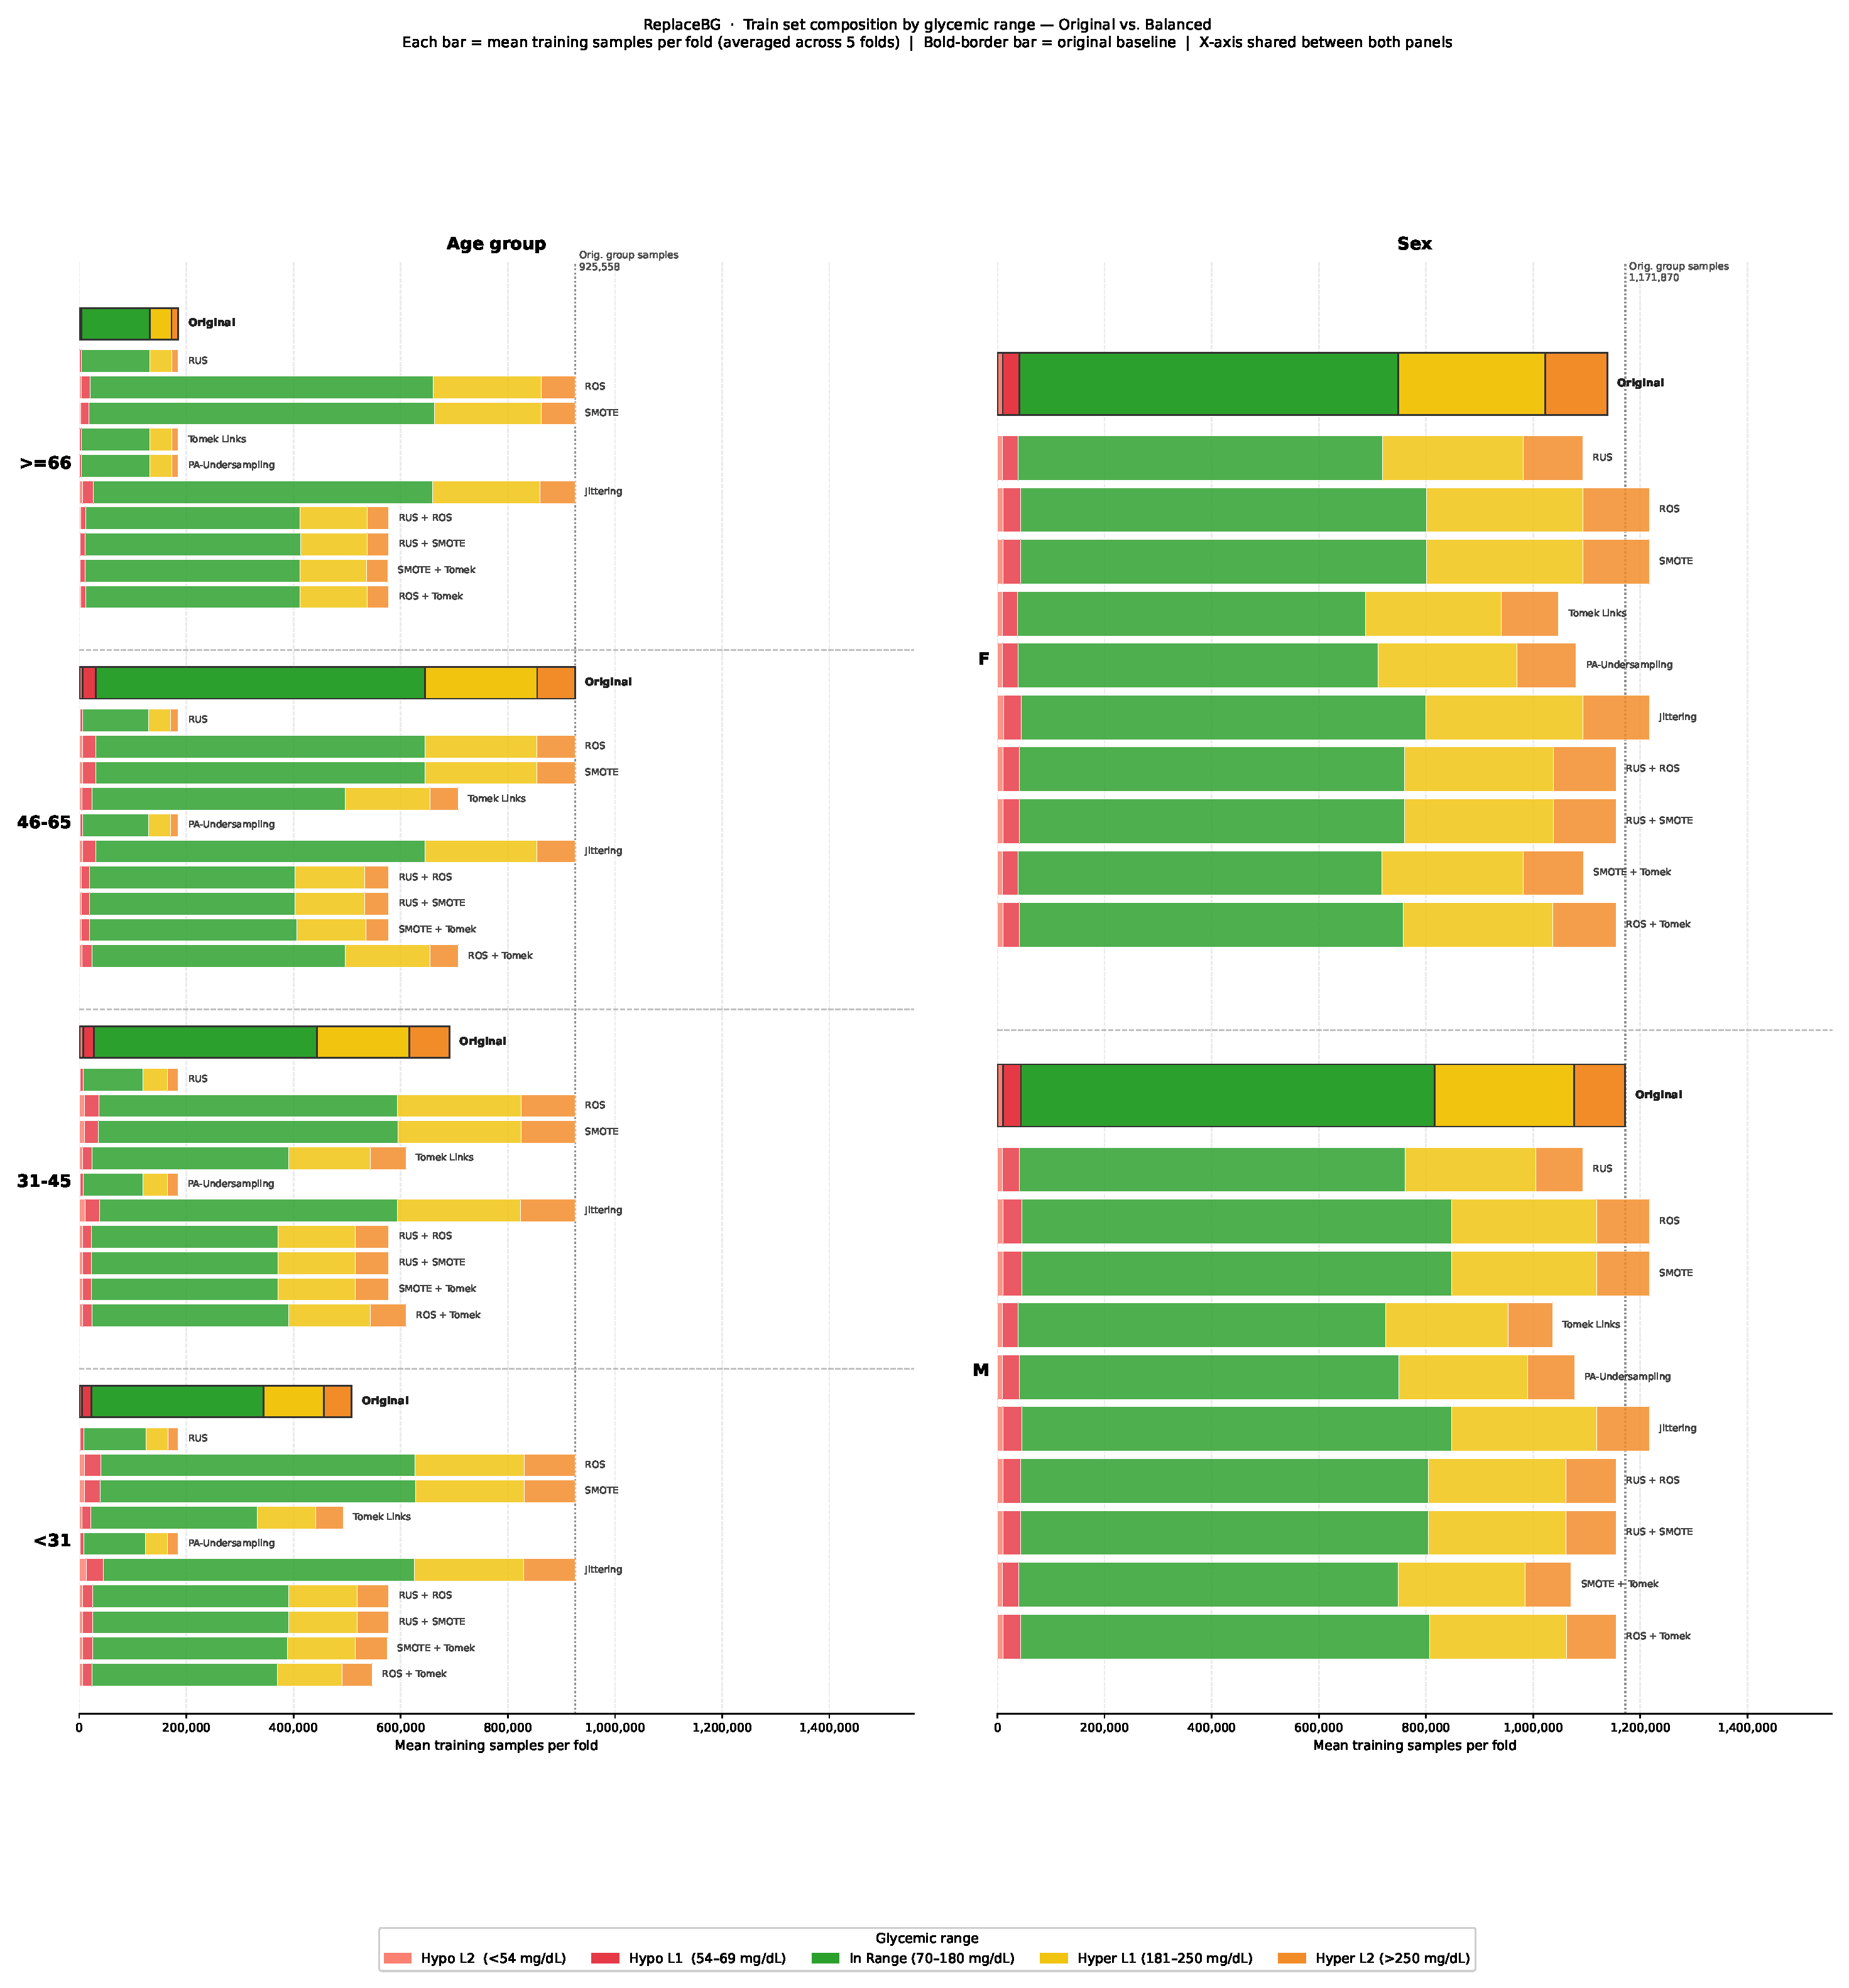
\includegraphics[width=\textwidth]{%
        ../../analysis_relief/outputs_clinical/stacked_bars_REPLACE-BG}
    \caption{Distribución glucémica del conjunto de entrenamiento de
             \textbf{REPLACE-BG} por técnica y dimensión. La homogeneidad
             de los seguimientos produce barras visualmente más uniformes
             entre técnicas que en los otros dos repositorios.}
    \label{fig:stacked_replacbg}
\end{figure}

REPLACE-BG presenta la distribución glucémica original más equilibrada de
los tres repositorios: el grupo de edad 46--65 (mayoritario) aporta
$\approx$925\,000 ventanas por \textit{fold}, y los rangos glucémicos se
distribuyen de forma más homogénea que en T1DiabetesGranada o DiaTrend,
coherente con el mejor TIR global documentado en el EDA ($\approx$57\,\%).
Las barras apiladas muestran que las técnicas de aumento generan incrementos
moderados y bien distribuidos entre rangos, mientras que las de reducción
producen barras más compactas pero con proporciones relativas similares al
original, reflejo de que el diseño controlado del ensayo REPLACE-BG minimiza
las diferencias glucémicas entre grupos demográficos.

\begin{figure}[H]
    \centering
    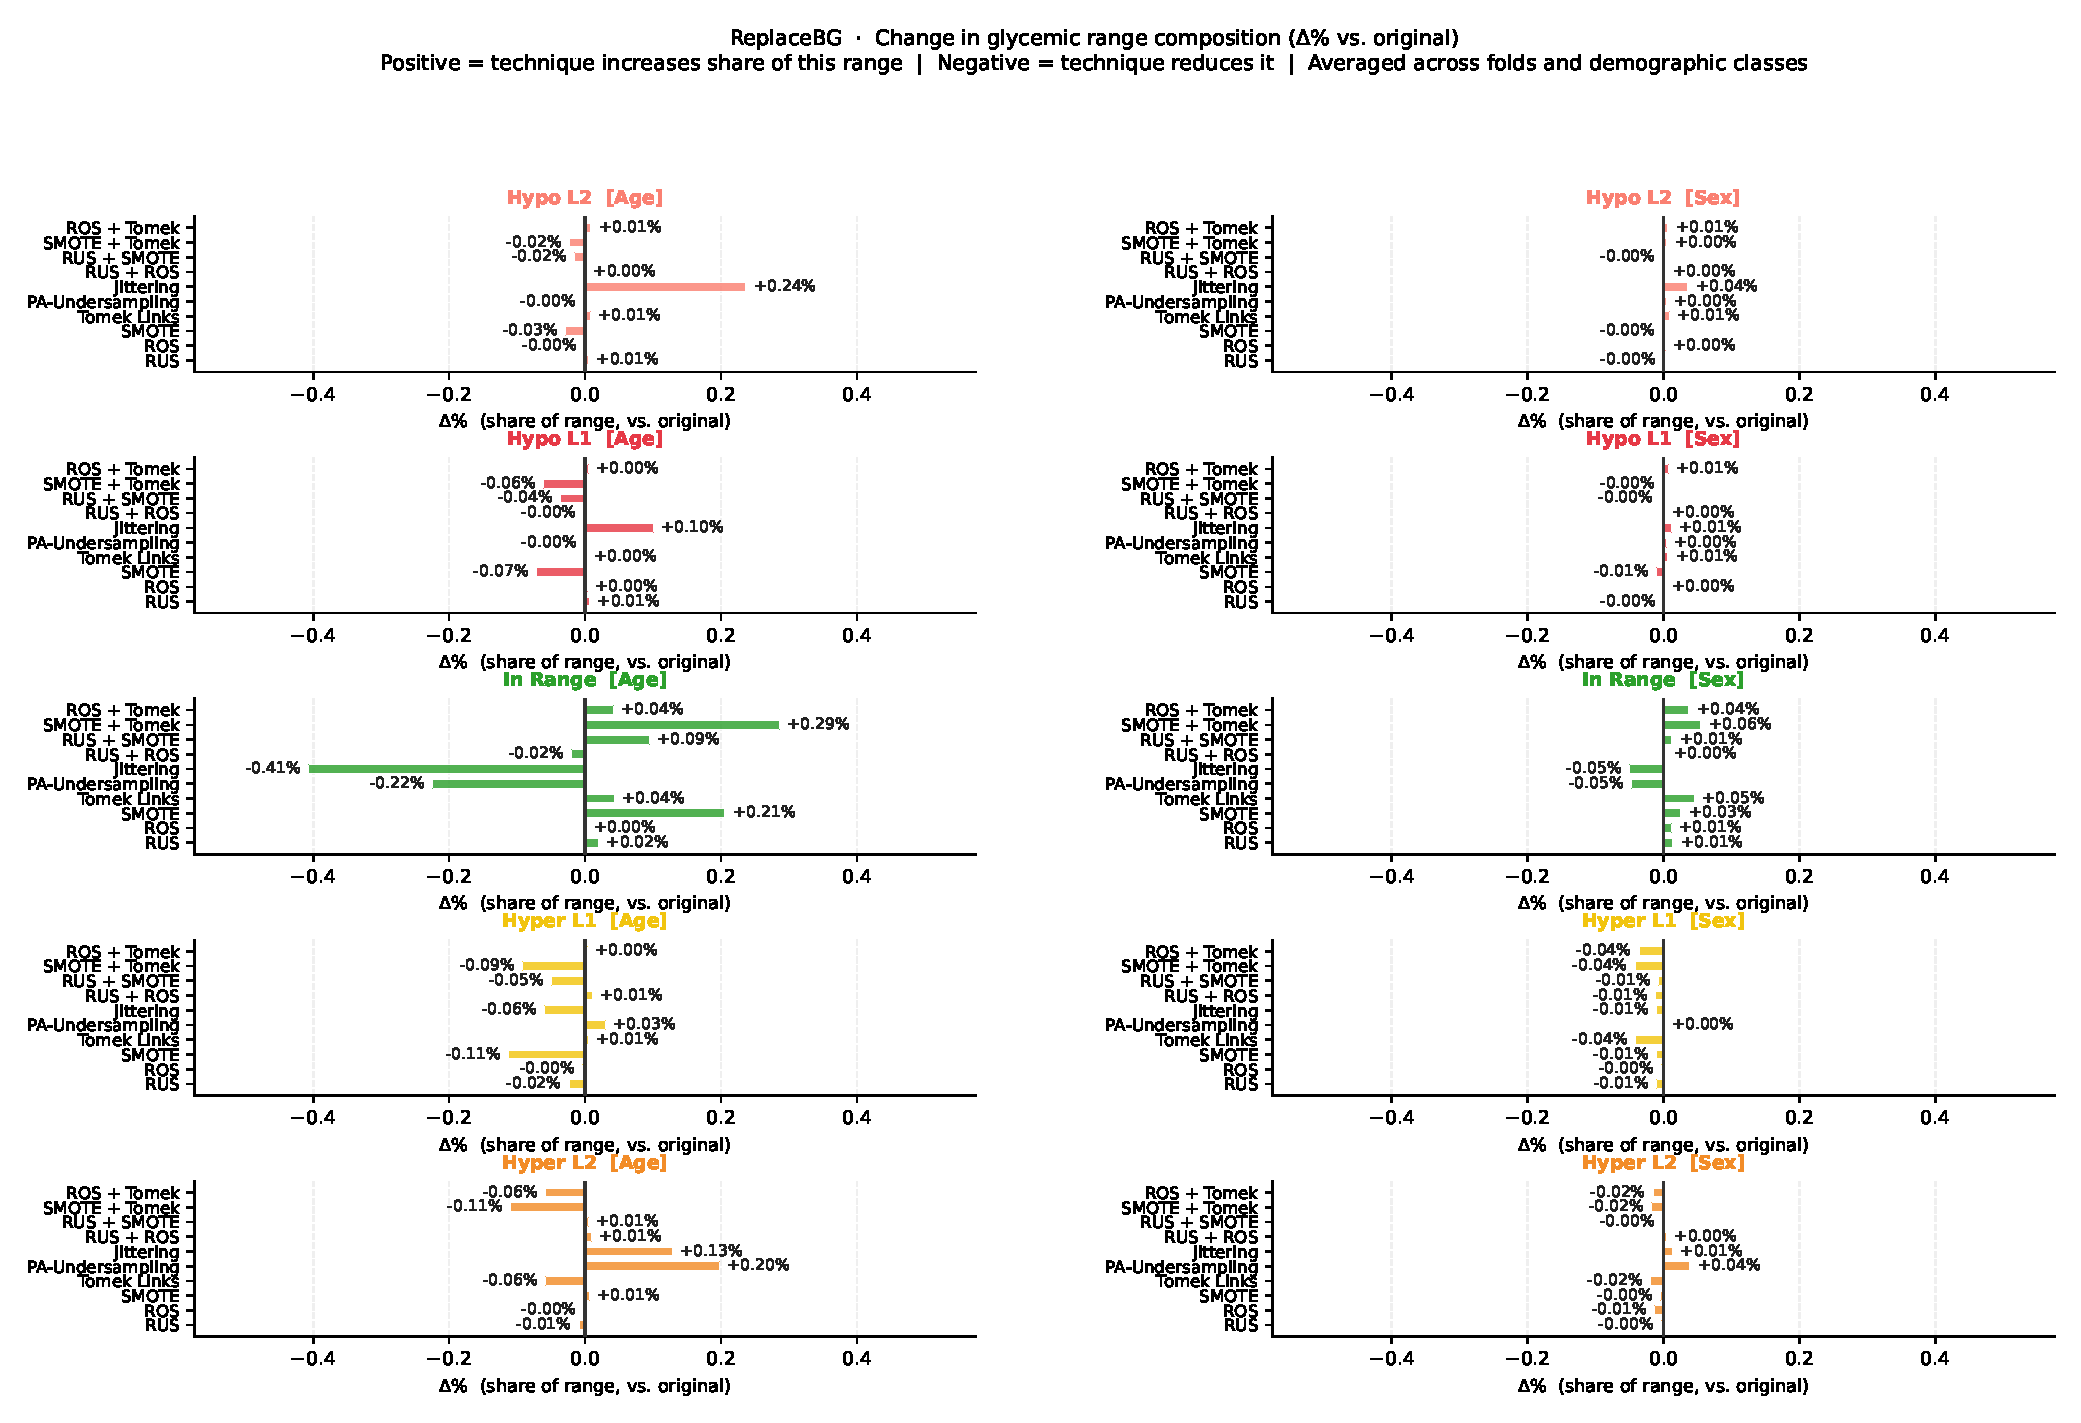
\includegraphics[width=\textwidth]{%
        ../../analysis_relief/outputs_clinical/delta_glycemic_REPLACE-BG}
    \caption{Variación $\Delta\%$ en la representación de rangos glucémicos
             para \textbf{REPLACE-BG}. Los cambios son los más moderados de
             los tres \textit{datasets}, confirmando que la homogeneidad de
             los seguimientos limita el impacto glucémico del balanceo
             demográfico.}
    \label{fig:delta_glycemic_replacbg}
\end{figure}

Las barras divergentes de la figura~\ref{fig:delta_glycemic_replacbg}
confirman que REPLACE-BG es el repositorio con menor impacto glucémico
del balanceo. En la dimensión edad, los cambios más relevantes afectan al
TIR: SMOTE+Tomek lo incrementa en $+0{,}29\%$ y RUS+SMOTE en $+0{,}09\%$,
mientras que PA-Undersampling lo reduce en $-0{,}22\%$ y Jittering en
$-0{,}41\%$ --- el único cambio negativo de TIR en este repositorio, y
también el más llamativo, sugiriendo que el perfil glucémico del grupo
$\geq$66 en REPLACE-BG (que Jittering amplifica) es proporcionalmente
más rico en rangos no-TIR que en los otros grupos. Para TBR-2, todos los
cambios son inferiores a $\pm 0{,}24\%$, con solo PA-Undersampling y
Jittering superando el umbral de $0{,}10\%$. En la dimensión sexo los
cambios son prácticamente nulos ($|\Delta\%| < 0{,}06\%$ en todos los
rangos salvo TAR-2 con PA-Undersampling, $+0{,}04\%$), lo que confirma
que el balanceo por sexo en REPLACE-BG no induce ninguna reorientación
glucémica apreciable.

\paragraph{Síntesis y conexión con los resultados de predicción.}
Los tres análisis anteriores permiten establecer una conclusión estructural
importante: el balanceo demográfico modifica la composición glucémica del
entrenamiento de forma sistemática pero de magnitud pequeña en todos los
repositorios, con cambios $\Delta\%$ que raramente superan $\pm 1\%$ en
cualquier rango individual. Esta pequeña magnitud no implica que el efecto
sea irrelevante clínicamente: en rangos de baja prevalencia como TBR-2
(hipoglucemia severa), un cambio de $+0{,}27\%$ en la representación puede
suponer una variación relativa del 10--20\,\% sobre la fracción original de
ese rango, lo que es suficiente para modificar la sensibilidad del modelo a
esos eventos. La sección~\ref{sec:efecto_balanceo_prediccion} analiza si
esos cambios de composición se traducen en diferencias medibles en las
métricas de predicción.


% ---------------------------------------------------------
\subsection{Trade-off clínico del balanceo: hipoglucemia, normoglucemia e hiperglucemia}
\label{subsec:tradeoff_clinico}
% ---------------------------------------------------------

El análisis de la subsección anterior cuantificó los cambios absolutos en la
composición glucémica del entrenamiento. Esta subsección adopta una perspectiva
clínica: para cada rango glucémico de interés, se analiza si el balanceo
consigue incrementar su representación en el entrenamiento \emph{sin} reducir
simultáneamente la normoglucemia (TIR), que es la métrica de control glucémico
de referencia en diabetes tipo 1. Este análisis de trade-off es relevante porque
un modelo que aprende a costa de reducir su exposición a ventanas en TIR puede
mejorar su sensibilidad a eventos extremos a expensas de deteriorar su precisión
en el rango más frecuente.

Cada figura de dispersión presenta tres paneles (uno por \textit{dataset}) con
los puntos posicionados en el espacio ($\Delta\%$ rango clínico, $\Delta\%$ TIR).
El cuadrante superior izquierdo ---fondo verde, etiquetado ``ideal''--- corresponde
a técnicas que incrementan TIR sin aumentar la exposición al rango clínico adverso;
el cuadrante inferior derecho es el escenario menos deseable. Los marcadores
distinguen la dimensión demográfica ($\circ$ = edad, $\square$ = sexo).

\paragraph{Trade-off TBR-2 (hipoglucemia severa, $<$54\,mg/dL) vs.\ TIR.}

\begin{figure}[H]
    \centering
    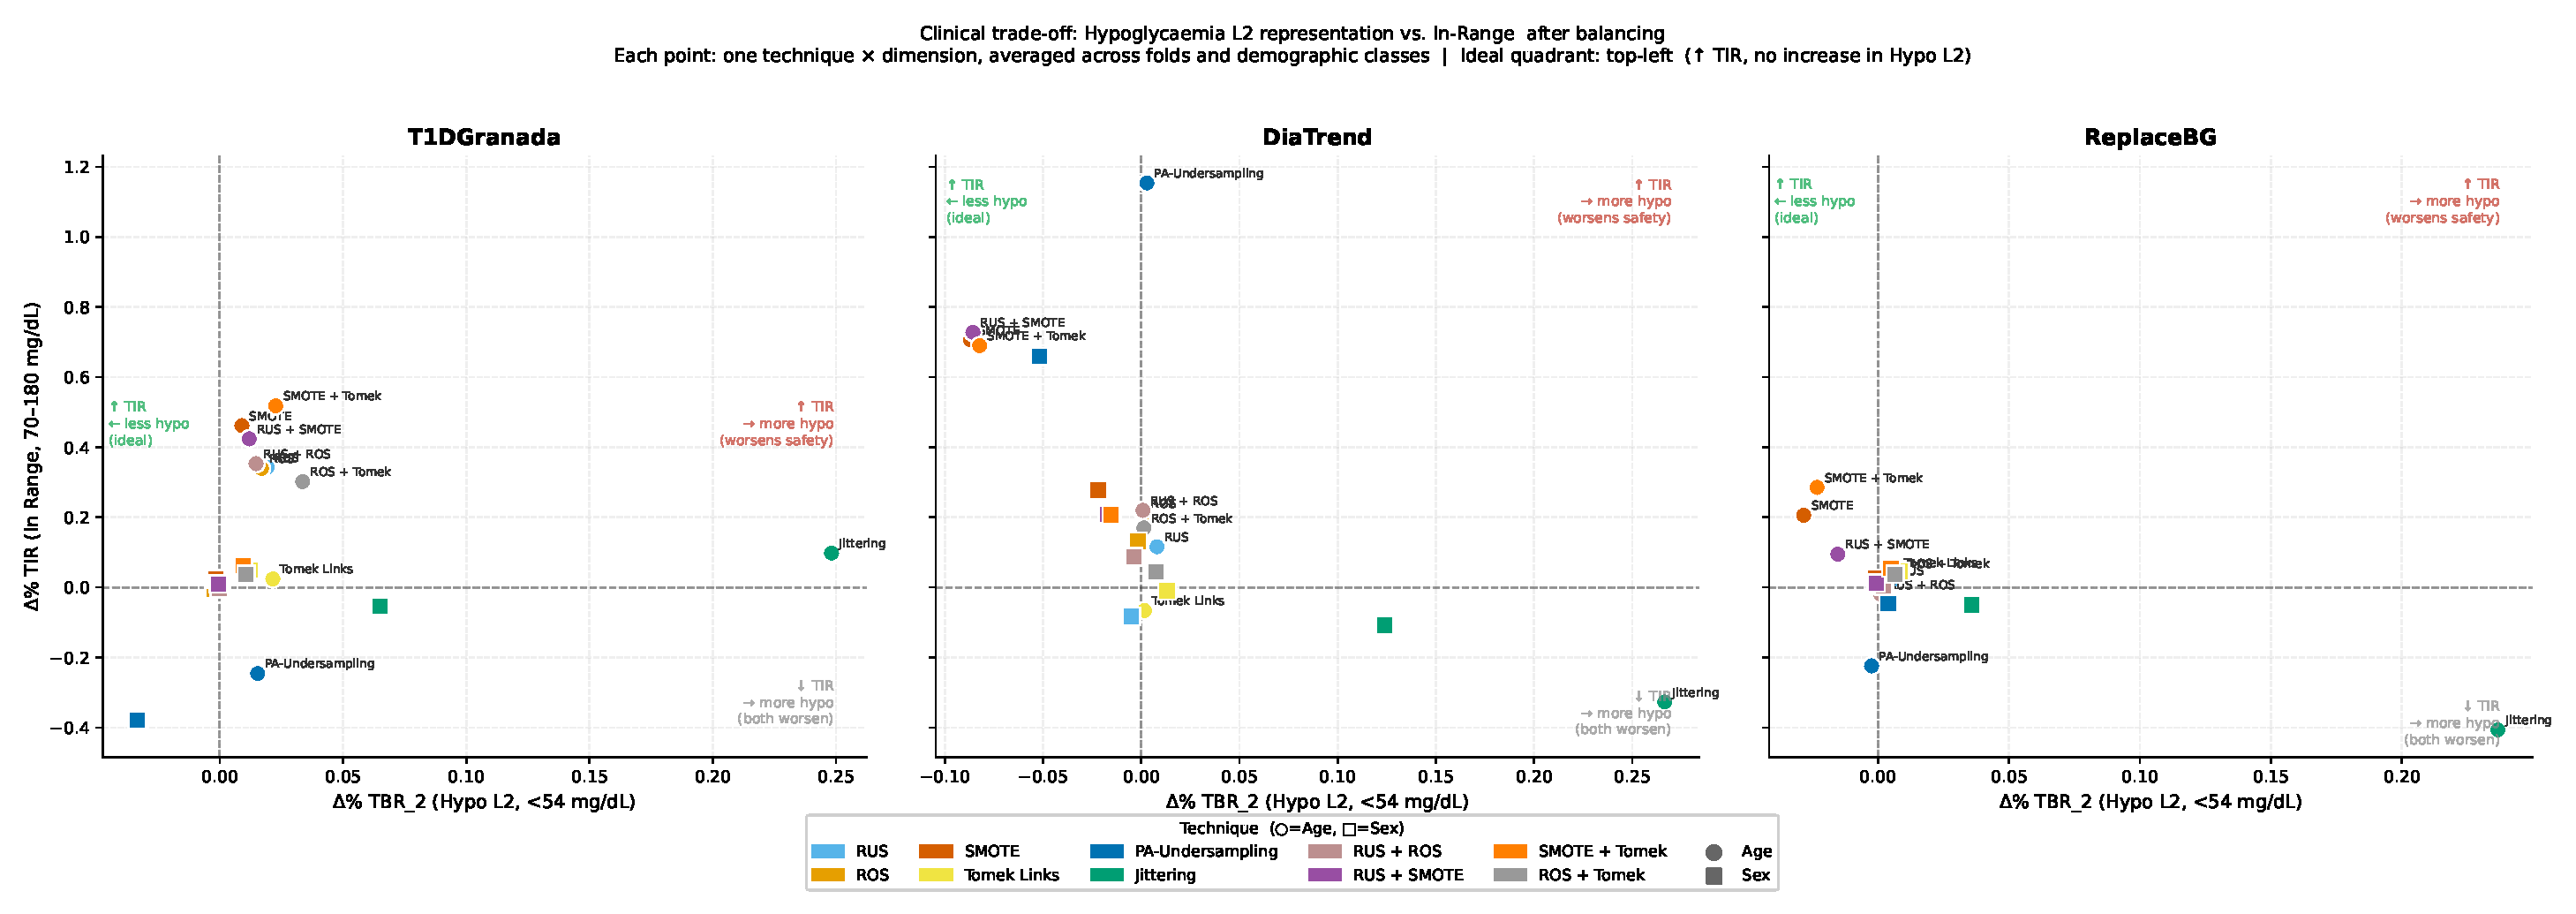
\includegraphics[width=\textwidth]{%
        ../../analysis_relief/outputs_clinical/tradeoff_tbr2_vs_tir}
    \caption{Trade-off clínico entre la variación de hipoglucemia severa
             ($\Delta\%$ TBR-2, eje $X$) y la variación de normoglucemia
             ($\Delta\%$ TIR, eje $Y$) tras aplicar cada técnica de balanceo,
             por \textit{dataset}. Cada punto representa una técnica $\times$
             dimensión demográfica ($\circ$\,=\,edad, $\square$\,=\,sexo).
             El cuadrante superior izquierdo (``ideal'') corresponde a
             técnicas que aumentan TIR sin incrementar la exposición a
             hipoglucemia severa.}
    \label{fig:tradeoff_tbr2}
\end{figure}

TBR-2 es el rango clínicamente más crítico: la hipoglucemia severa
($<$54\,mg/dL) representa un riesgo inmediato para el paciente y su
infrarrepresentación en el entrenamiento puede limitar la capacidad del modelo
para anticipar estos eventos. El scatter de la figura~\ref{fig:tradeoff_tbr2}
revela patrones muy distintos según el repositorio.

En \textbf{T1DiabetesGranada} todos los puntos se agrupan en torno al origen
con desplazamientos $|\Delta\%| < 0{,}25\%$ en ambos ejes, pero el patrón
predominante es el cuadrante superior derecho: la mayoría de técnicas incrementan
simultáneamente TBR-2 y TIR, siendo Jittering (dimensión edad) el caso más
extremo ($\Delta\%\,\text{TBR-2} \approx +0{,}25\%$, $\Delta\%\,\text{TIR}
\approx +0{,}10\%$). PA-Undersampling es la única técnica que se aproxima al
cuadrante ideal de forma clara en dimensión sexo, incrementando TIR
($+0{,}66\%$) con un cambio mínimo en TBR-2. Tomek Links se sitúa en el
cuadrante inferior izquierdo (reduce ambos), mientras que RUS queda próximo
al origen. Ninguna técnica consigue un posicionamiento inequívocamente ideal
en este dataset.

En \textbf{DiaTrend} la dispersión es mucho mayor, coherente con la magnitud
de los cambios documentados en la figura~\ref{fig:delta_glycemic_diatrend}.
PA-Undersampling (dimensión edad) se posiciona claramente en el cuadrante
superior izquierdo ($\Delta\%\,\text{TIR} \approx +1{,}15\%$,
$\Delta\%\,\text{TBR-2} \approx 0\%$), siendo la única técnica que se acerca
al ideal en este repositorio. Jittering (edad) se ubica en el cuadrante
superior derecho ($+0{,}27\%$ TBR-2, $+0{,}33\%$ TIR), lo que supone una
mejora de ambos rangos simultáneamente --- un resultado favorable aunque no
estrictamente ideal. Las técnicas de reducción (RUS, dimensión edad) caen en
el cuadrante inferior izquierdo, con reducción de TBR-2 y TIR. Los puntos de
dimensión sexo quedan muy próximos al origen en todos los casos, confirmando
que el desequilibrio de sexo en DiaTrend no produce reorientaciones glucémicas
relevantes en TBR-2.

En \textbf{REPLACE-BG} todos los puntos se concentran cerca del origen con
escala notablemente más comprimida ($|\Delta\%\,\text{TBR-2}| < 0{,}24\%$),
y el patrón predominante es el cuadrante superior derecho para la dimensión
edad (incremento moderado de ambos TBR-2 y TIR), con Jittering como caso
más desplazado. La dimensión sexo produce puntos prácticamente en el origen,
sin trade-off apreciable.

\paragraph{Trade-off TBR-1 (hipoglucemia leve, 54--69\,mg/dL) vs.\ TIR.}

\begin{figure}[H]
    \centering
    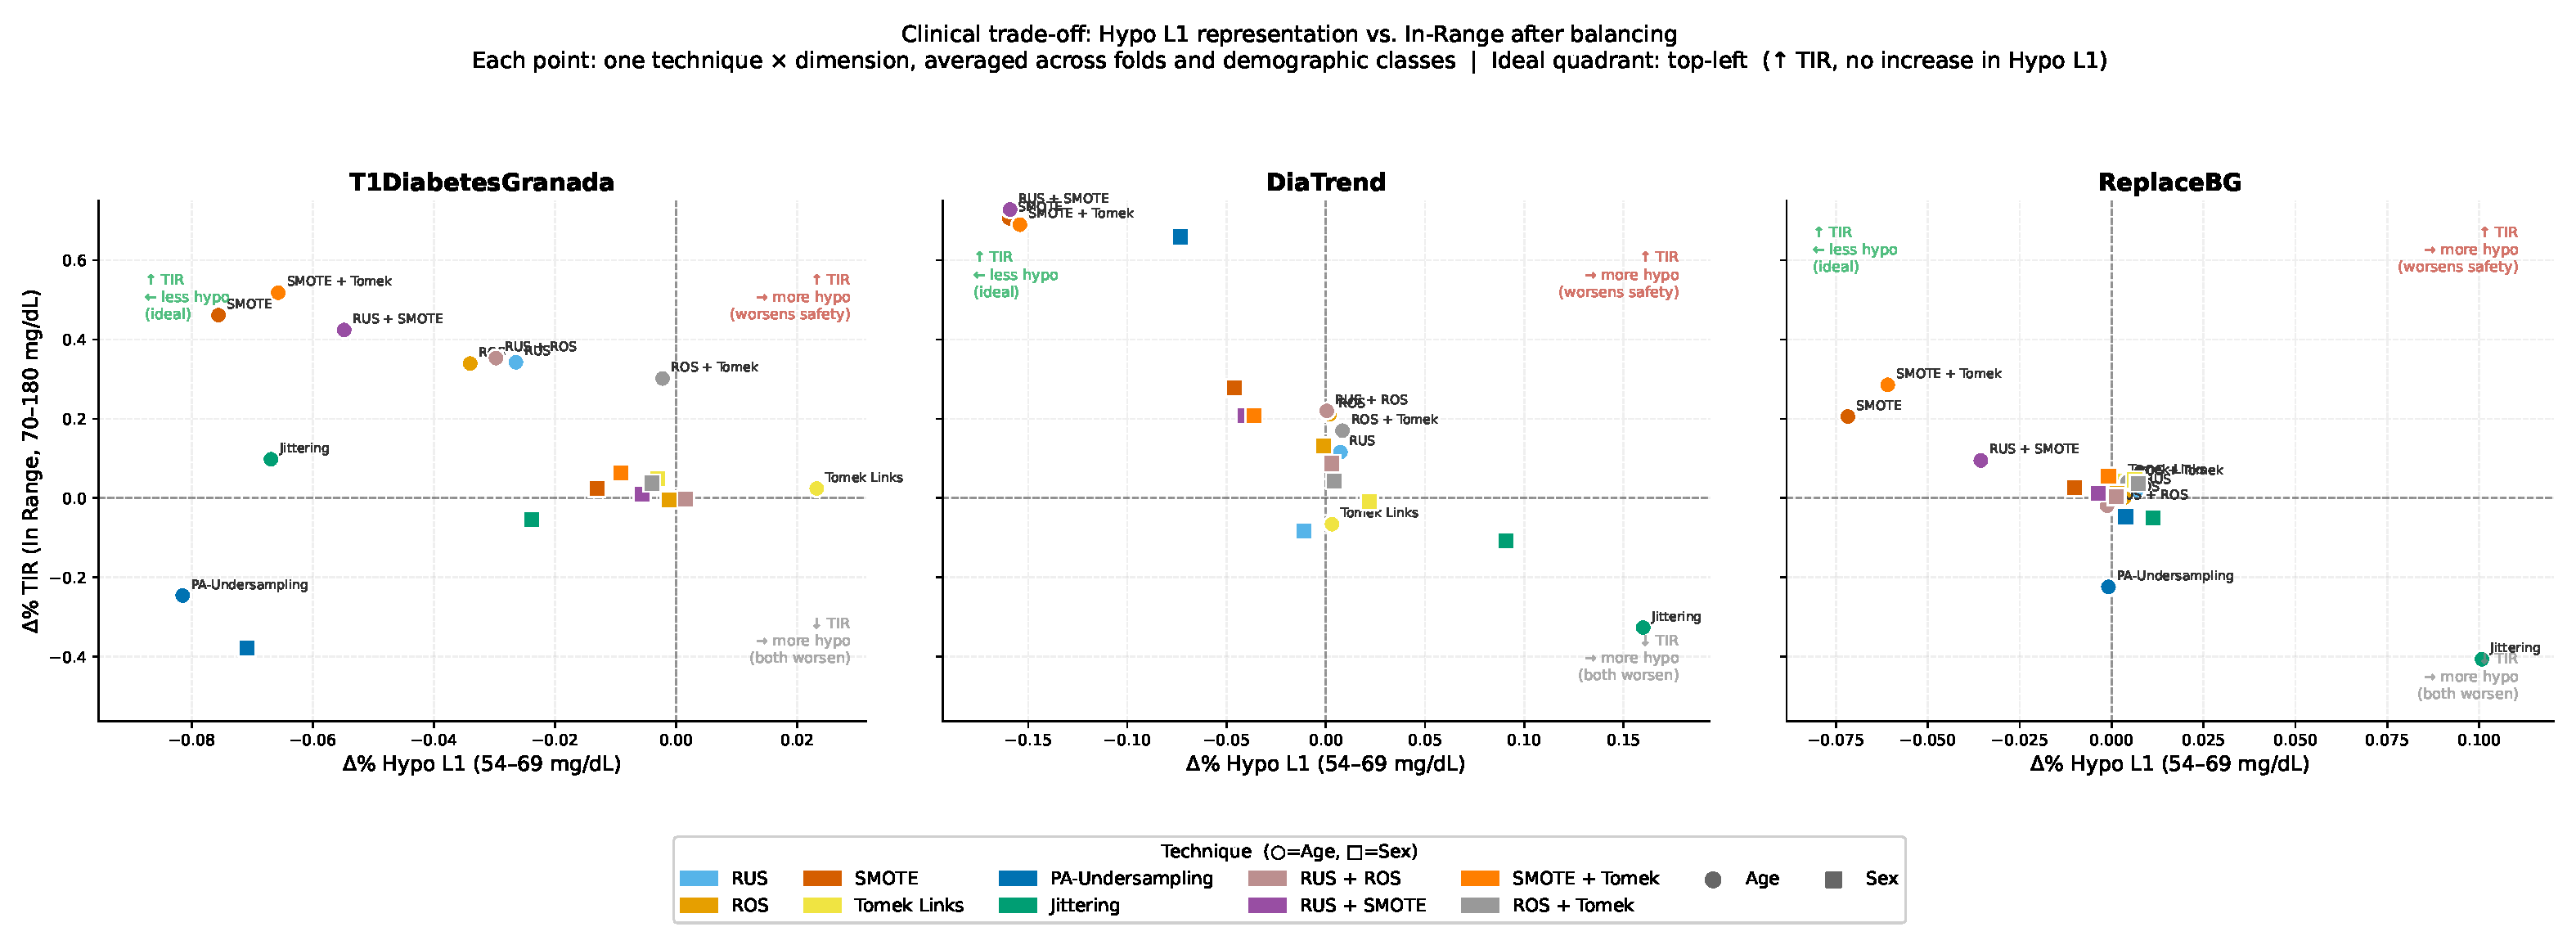
\includegraphics[width=\textwidth]{%
        ../../analysis_relief/outputs_clinical/tradeoff_tbr1_vs_tir}
    \caption{Trade-off clínico entre la variación de hipoglucemia leve
             ($\Delta\%$ TBR-1, eje $X$) y la variación de normoglucemia
             ($\Delta\%$ TIR, eje $Y$). Mismas convenciones que la
             figura~\ref{fig:tradeoff_tbr2}.}
    \label{fig:tradeoff_tbr1}
\end{figure}

El patrón por técnica en TBR-1 es cualitativamente similar al de TBR-2 en
los tres repositorios, pero con algunas diferencias relevantes. En
\textbf{T1DiabetesGranada} la dispersión aumenta ligeramente respecto a TBR-2:
PA-Undersampling (edad) se desplaza hacia el cuadrante ideal con mayor claridad
($\Delta\%\,\text{TIR} \approx +1{,}15\%$, $\Delta\%\,\text{TBR-1}$ negativo
o nulo), mientras que SMOTE y RUS+SMOTE (edad) se sitúan en el cuadrante
inferior izquierdo (reducen TBR-1 y apenas modifican TIR). Jittering mantiene
su posición en el cuadrante superior derecho pero con un incremento de TBR-1
más pronunciado que el de TBR-2, lo que indica que su efecto de aumento es
proporcionalmente mayor en hipoglucemia leve.

En \textbf{DiaTrend} la lectura cambia respecto a TBR-2: ROS, SMOTE y Jittering
(dimensión edad) se desplazan hacia el cuadrante superior derecho con
$\Delta\%\,\text{TBR-1} > 0$ y $\Delta\%\,\text{TIR} > 0$, lo que sugiere
que al amplificar el grupo $\geq$66 se introducen más ventanas en hipoglucemia
leve de lo que sucedía con la severa. PA-Undersampling mantiene su posición
favorable ($\Delta\%\,\text{TIR}$ alto, $\Delta\%\,\text{TBR-1}$ próximo a
cero o negativo). Las técnicas de reducción siguen en el cuadrante inferior
izquierdo. En \textbf{REPLACE-BG} el patrón es análogo al de TBR-2 con escala
similar, sin diferencias cualitativas notables entre rangos de hipoglucemia.

En conjunto, TBR-1 y TBR-2 muestran el mismo ranking de técnicas por
proximidad al cuadrante ideal: PA-Undersampling lidera en DiaTrend, mientras
que en T1DiabetesGranada y REPLACE-BG ninguna técnica consigue un
posicionamiento nítidamente favorable.

\paragraph{Trade-off TAR-1 (hiperglucemia leve, 181--250\,mg/dL) vs.\ TIR.}

\begin{figure}[H]
    \centering
    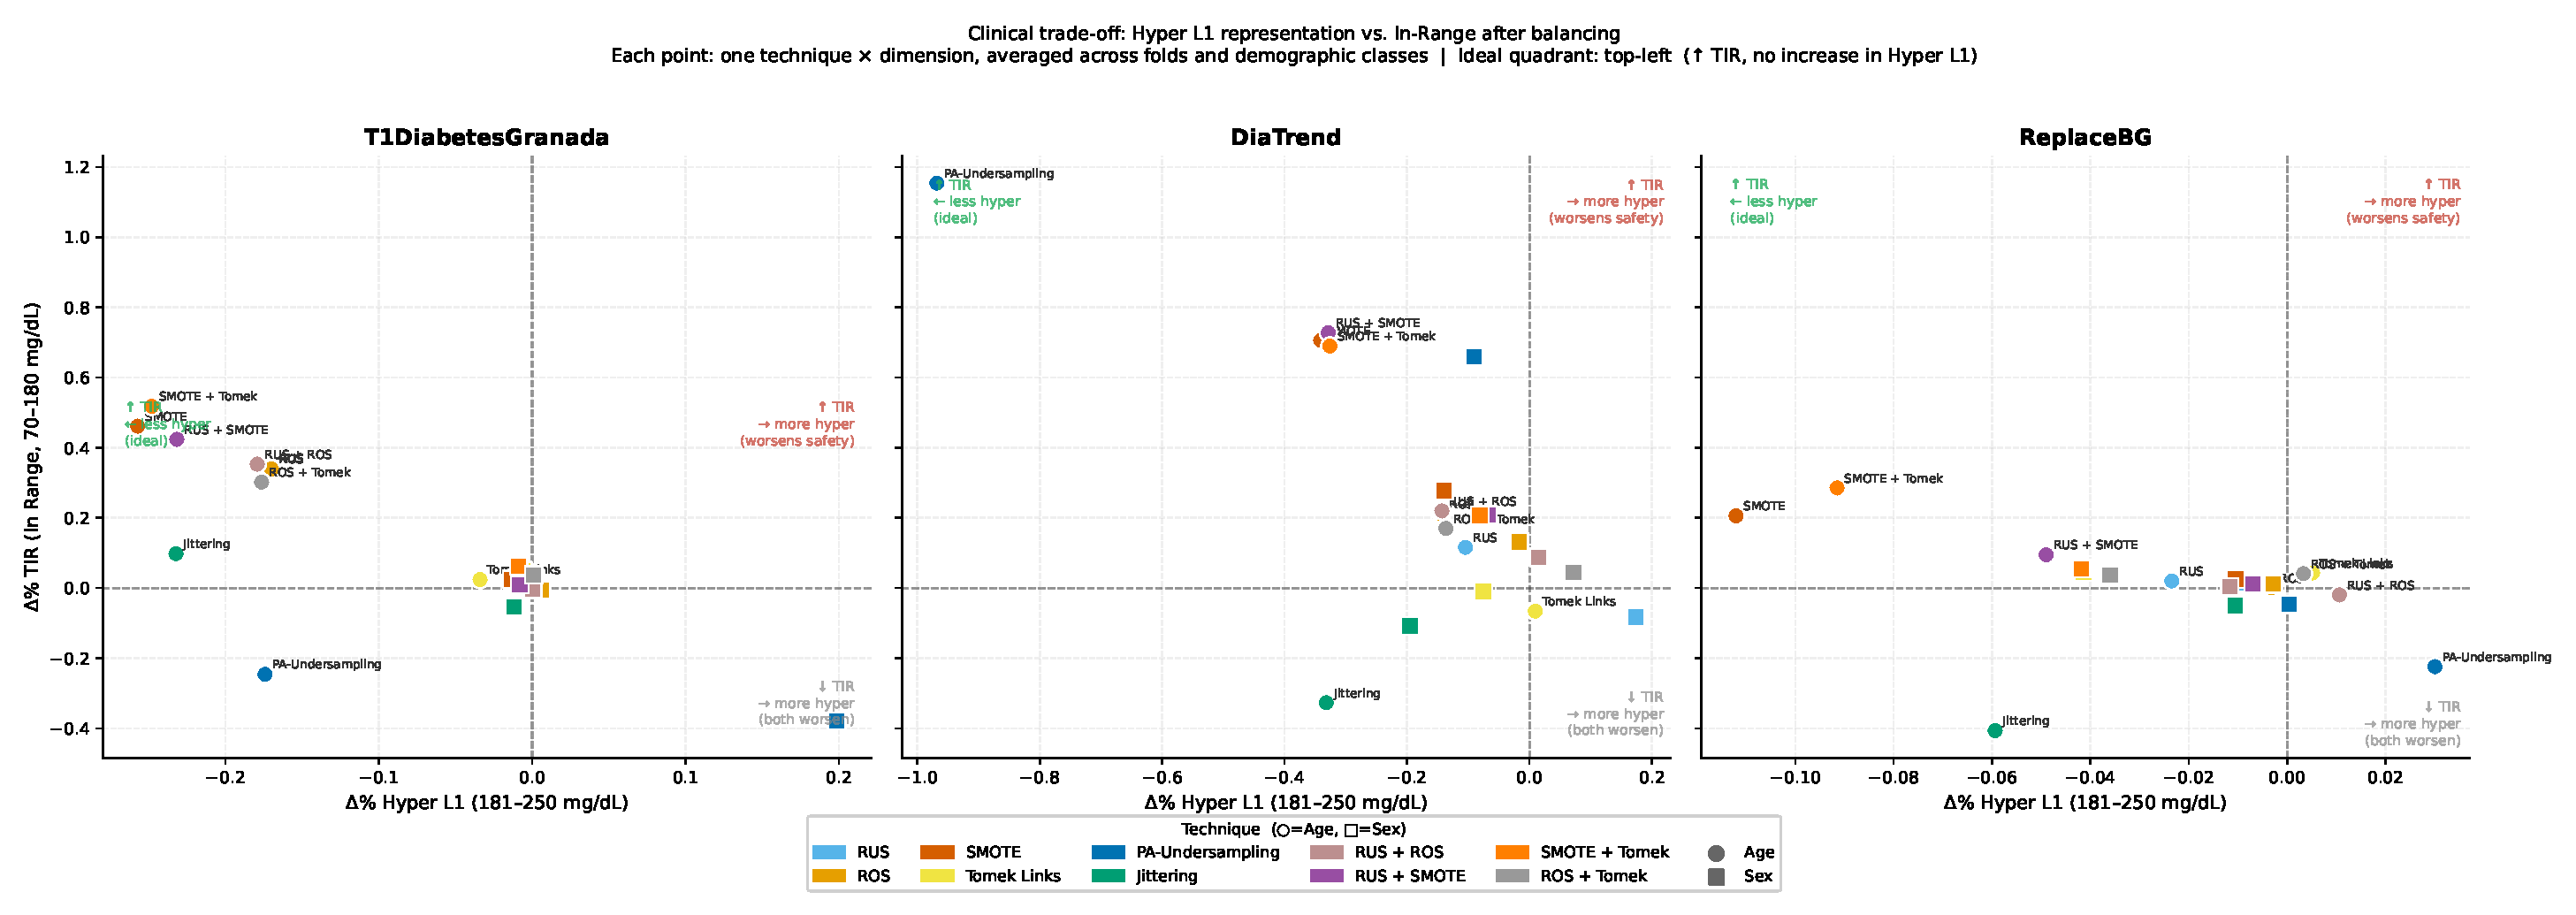
\includegraphics[width=\textwidth]{%
        ../../analysis_relief/outputs_clinical/tradeoff_tar1_vs_tir}
    \caption{Trade-off clínico entre la variación de hiperglucemia leve
             ($\Delta\%$ TAR-1, eje $X$) y la variación de normoglucemia
             ($\Delta\%$ TIR, eje $Y$). En este scatter el cuadrante ideal
             (superior izquierdo) corresponde a técnicas que aumentan TIR
             reduciendo simultáneamente la exposición a hiperglucemia leve.}
    \label{fig:tradeoff_tar1}
\end{figure}

La lectura del trade-off con TAR-1 invierte la dirección deseable en el eje
$X$: aquí el cuadrante ideal es el superior izquierdo, donde las técnicas
reducen la hiperglucemia leve al tiempo que aumentan el TIR. En
\textbf{T1DiabetesGranada} la mayoría de técnicas de aumento (ROS, SMOTE,
Jittering, RUS+ROS, RUS+SMOTE) se posicionan claramente en ese cuadrante
(dimensión edad), con reducciones de TAR-1 de hasta $-0{,}26\%$ y ganancias
de TIR de hasta $+0{,}46\%$. PA-Undersampling se sitúa en el extremo superior
izquierdo con la mayor ganancia de TIR ($\approx +1{,}15\%$) y una reducción
de TAR-1 de $-0{,}97\%$, siendo la técnica más favorable en este eje. RUS
queda próximo al origen con $\Delta\%\,\text{TAR-1} \approx -0{,}10\%$ y
$\Delta\%\,\text{TIR}$ ligeramente positivo. Tomek Links es la única técnica
neutral ($|\Delta\%| < 0{,}07\%$ en ambos ejes). La dimensión sexo produce
puntos más próximos al origen pero con el mismo patrón cualitativo.

En \textbf{DiaTrend} la dispersión es la mayor de los tres repositorios:
PA-Undersampling (edad) alcanza $\Delta\%\,\text{TIR} \approx +1{,}15\%$ con
una reducción de TAR-1 de $\approx -0{,}97\%$, el posicionamiento más favorable
de todos. ROS, SMOTE y Jittering (edad) se ubican en el cuadrante superior
izquierdo con reducciones de TAR-1 entre $-0{,}33\%$ y $-0{,}14\%$ y ganancias
de TIR entre $+0{,}12\%$ y $+0{,}33\%$. Las técnicas de reducción (RUS) caen
en el cuadrante inferior izquierdo (reducen TAR-1 pero también TIR).
En \textbf{REPLACE-BG} todos los puntos se concentran con $\Delta\%\,\text{TAR-1}$
entre $-0{,}11\%$ y $+0{,}03\%$, sin diferencias clínicamente relevantes entre
técnicas.

\paragraph{Trade-off TAR-2 (hiperglucemia severa, $>$250\,mg/dL) vs.\ TIR.}

\begin{figure}[H]
    \centering
    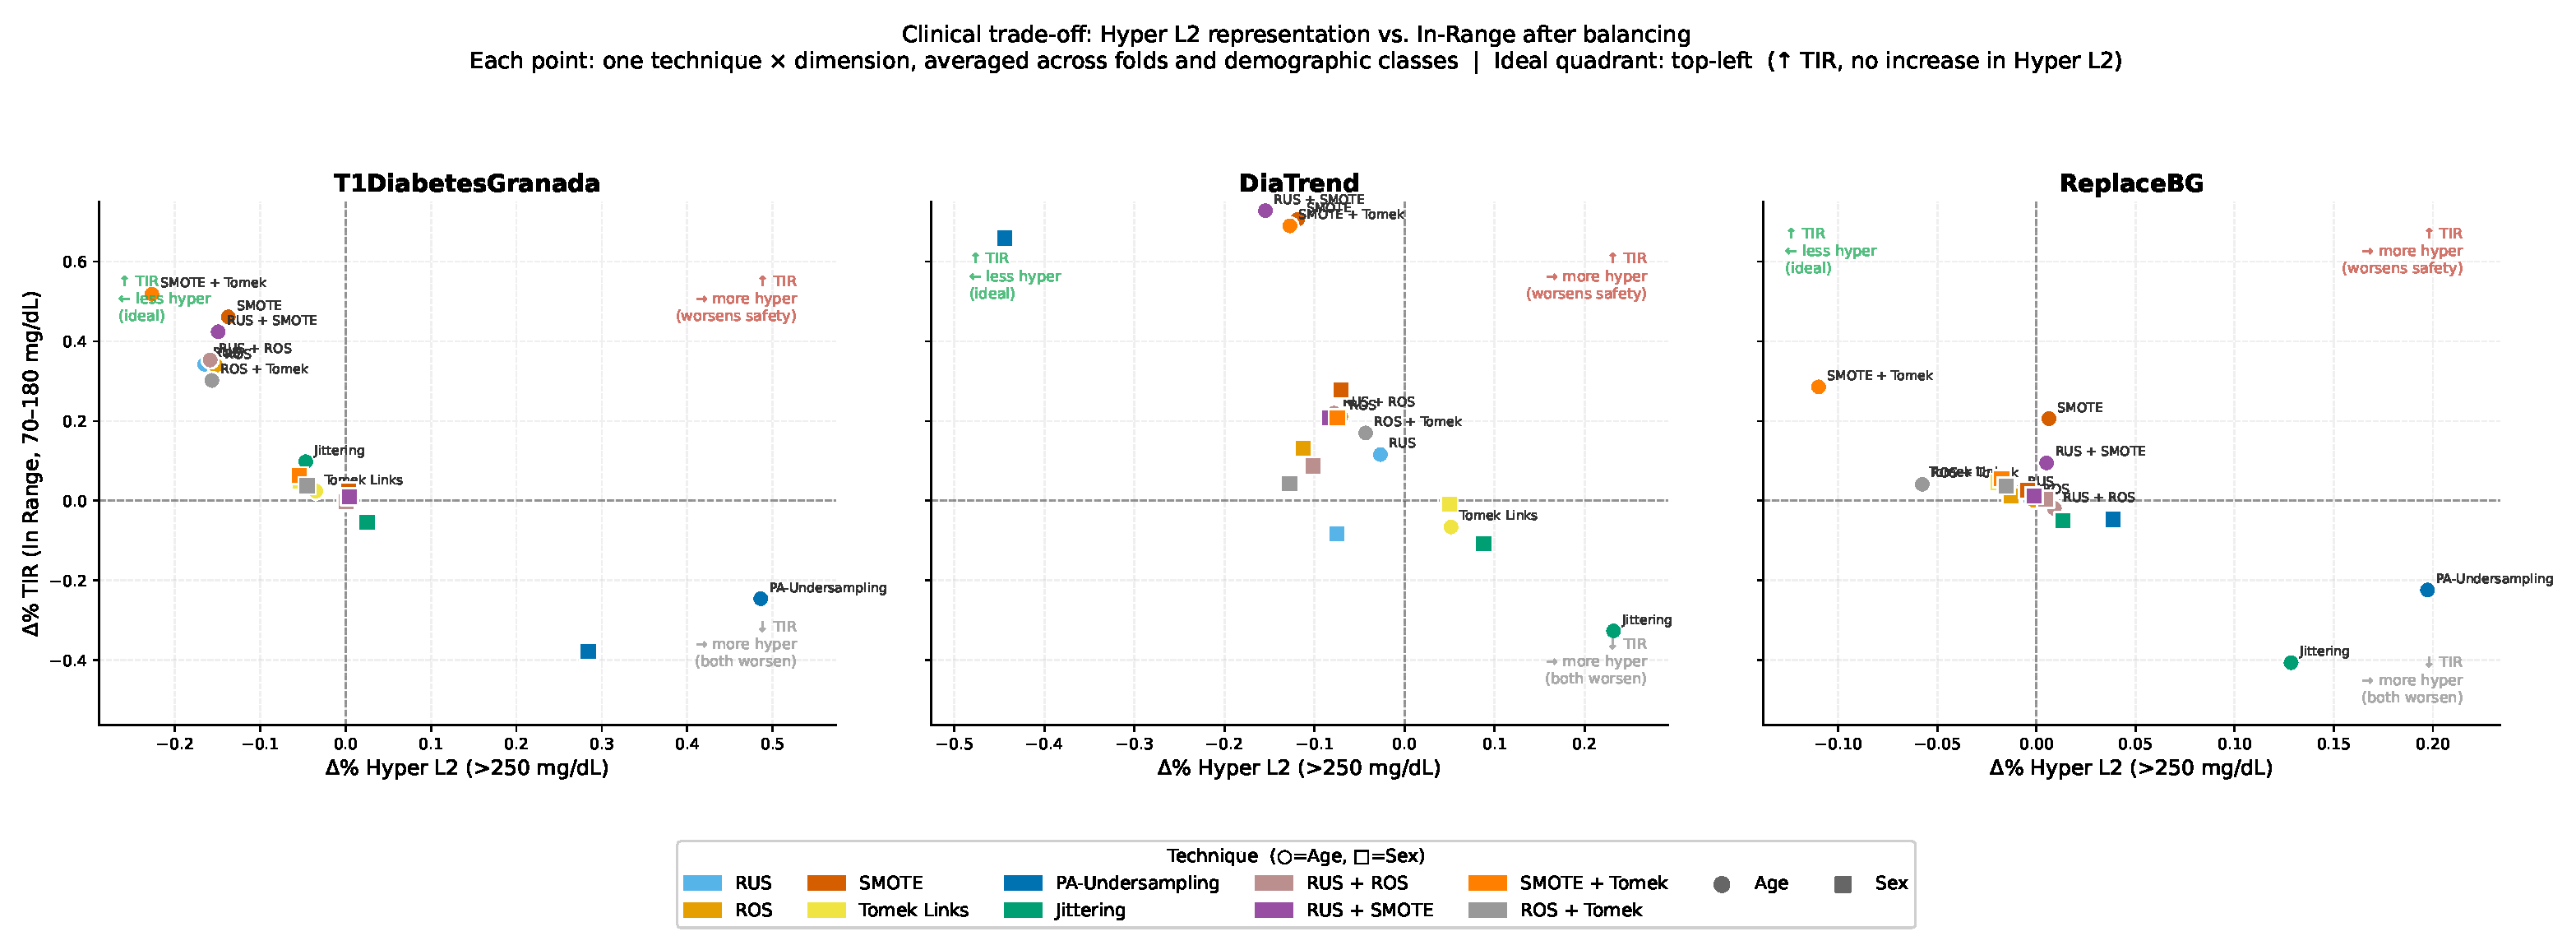
\includegraphics[width=\textwidth]{%
        ../../analysis_relief/outputs_clinical/tradeoff_tar2_vs_tir}
    \caption{Trade-off clínico entre la variación de hiperglucemia severa
             ($\Delta\%$ TAR-2, eje $X$) y la variación de normoglucemia
             ($\Delta\%$ TIR, eje $Y$). El cuadrante ideal (superior
             izquierdo) corresponde a técnicas que incrementan TIR reduciendo
             la exposición a hiperglucemia severa.}
    \label{fig:tradeoff_tar2}
\end{figure}

El análisis de TAR-2 completa el panorama glucémico y revela el trade-off
más pronunciado de todos los rangos en T1DiabetesGranada. En este repositorio,
PA-Undersampling (edad) se posiciona en el extremo superior derecho: consigue
la mayor ganancia de TIR ($\approx +1{,}15\%$) pero a costa de un incremento
de TAR-2 de $\approx +0{,}49\%$, el mayor aumento de hiperglucemia severa
observado en cualquier técnica y dataset. Este comportamiento es coherente con
la lógica de PA-Undersampling en T1DiabetesGranada: al eliminar
desproporcionadamente ventanas del grupo 46--65 (que tiene un perfil glucémico
con menor TAR-2), el train resultante queda con mayor representación de
perfiles de pacientes mayores que presentan, paradójicamente, más episodios
de hiperglucemia severa. Jittering (edad) también se sitúa en el cuadrante
superior derecho ($+0{,}23\%$ TAR-2, $+0{,}10\%$ TIR), mientras que SMOTE
y ROS+SMOTE quedan en el cuadrante superior izquierdo (ideal): reducen TAR-2
entre $-0{,}14\%$ y $-0{,}23\%$ con ganancias de TIR de hasta $+0{,}46\%$.

En \textbf{DiaTrend} el patrón se invierte respecto a T1DiabetesGranada: la
mayoría de técnicas de aumento se posicionan en el cuadrante superior izquierdo
(reducen TAR-2 y aumentan TIR), con PA-Undersampling de nuevo en el extremo
pero ahora en el cuadrante ideal ($\Delta\%\,\text{TAR-2} \approx -0{,}18\%$,
$\Delta\%\,\text{TIR} \approx +1{,}15\%$). RUS cae en el cuadrante inferior
izquierdo. En \textbf{REPLACE-BG} los puntos de dimensión edad se distribuyen
entre los cuadrantes superior izquierdo (SMOTE: $-0{,}11\%$ TAR-2) y superior
derecho (PA-Undersampling: $+0{,}20\%$ TAR-2), con amplitudes similares a las
de TAR-1.

\paragraph{Síntesis del análisis de trade-off.}
El conjunto de los cuatro scatters permite extraer tres conclusiones
transversales. Primera: \textbf{ninguna técnica domina en todos los rangos y
datasets simultáneamente}; las técnicas que se aproximan al cuadrante ideal
en un rango tienden a alejarse en otro, confirmando que el trade-off glucémico
es inherente al mecanismo de balanceo y no un artefacto de una técnica
concreta. Segunda: \textbf{DiaTrend es el único repositorio donde el
posicionamiento en los scatters es clínicamente informativo}; en T1DiabetesGranada
y REPLACE-BG la magnitud de los cambios es tan pequeña que todos los puntos
caen dentro de un margen de $\pm 0{,}5\%$ que difícilmente se traduce en
diferencias de rendimiento estadísticamente detectables. Tercera: \textbf{la
dimensión demográfica (edad vs.\ sexo) determina la magnitud pero no la
dirección del trade-off}; los puntos de sexo son sistemáticamente más próximos
al origen que los de edad, pero comparten el mismo cuadrante en prácticamente
todos los casos, lo que indica que el mecanismo glucémico subyacente es el
mismo independientemente de la dimensión de balanceo utilizada.


% =========================================================
\section{Impacto del balanceo sobre el rendimiento del modelo LSTM}
\label{sec:analisis_mejora}
% =========================================================

Habiendo caracterizado en detalle cómo cada técnica de balanceo modifica el
conjunto de entrenamiento ---en tamaño, composición demográfica y distribución
glucémica---, esta sección evalúa si dichas modificaciones se traducen en
cambios medibles en el rendimiento predictivo del modelo LSTM. El análisis
se estructura en tres niveles de creciente especificidad: primero se examina
la distribución global de métricas entre técnicas y \textit{datasets}, que
permite identificar el rango de variación observable y la estabilidad inter-fold
de cada condición; a continuación se cuantifica el cambio respecto al
\textit{baseline} original mediante el tamaño del efecto de Cohen; finalmente
se aplican contrastes estadísticos no paramétricos (Friedman y Nemenyi
post-hoc) para determinar qué diferencias son estadísticamente significativas.
A lo largo de los tres niveles se prioriza la interpretación clínica ---con
especial atención al comportamiento en los rangos de hipoglucemia (TBR-2,
TBR-1) y al error global (ENTIRE)--- sobre las métricas de regresión puras.

% ---------------------------------------------------------
\subsection{Distribución global de métricas por técnica}
\label{subsec:distribucion_metricas}
% ---------------------------------------------------------

Esta subsección examina la distribución del RMSE entre los cinco \textit{folds}
para cada técnica de balanceo, con el objetivo de caracterizar tanto el nivel
central de rendimiento como su variabilidad inter-fold. Una técnica puede
obtener una mediana de RMSE comparable al \textit{baseline} pero con una
dispersión mucho mayor entre folds, lo que la haría clínicamente menos fiable
en un escenario de despliegue real.

\begin{figure}[H]
    \centering
    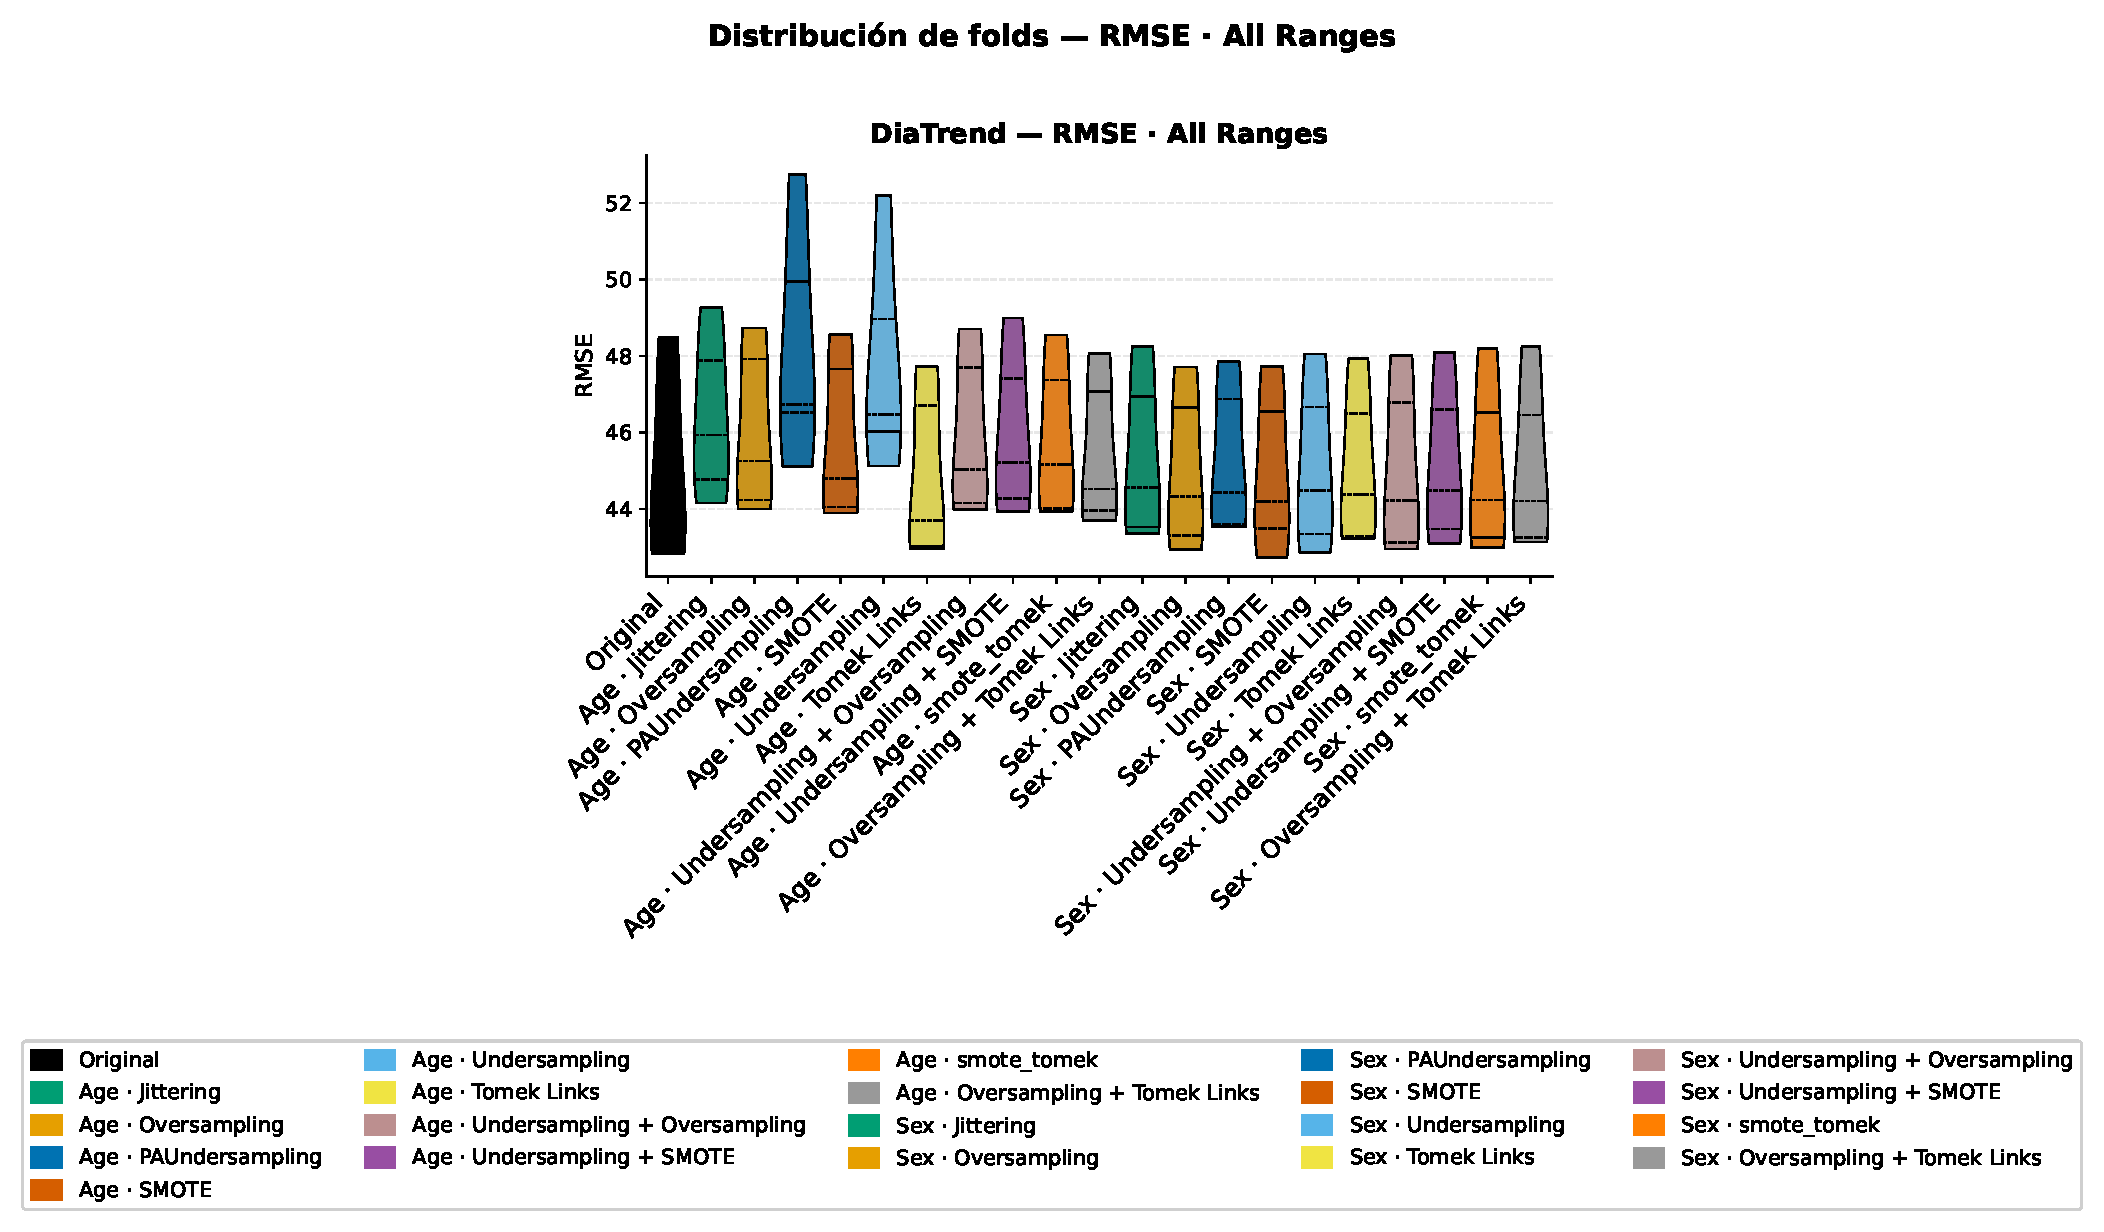
\includegraphics[width=\textwidth]{%
        ../../analysis_relief/outputs/figures/distributions/dist_RMSE_ENTIRE}
    \caption{Distribución del RMSE sobre el conjunto completo de ventanas
             (\textit{ENTIRE}) por técnica de balanceo y \textit{dataset}.
             Cada violín resume la distribución entre los 5 \textit{folds};
             la línea discontinua interior indica la mediana y las líneas
             externas el rango intercuartílico. La condición \textit{original}
             (negro) aparece como referencia.}
    \label{fig:dist_rmse_entire}
\end{figure}

\paragraph{RMSE global (ENTIRE).}
En \textbf{T1DiabetesGranada} la mediana de RMSE en la condición original es
$37{,}80 \pm 0{,}81$\,mg/dL y permanece notablemente estable entre todas las
condiciones balanceadas: los valores oscilan entre $37{,}56$ (PA-Undersampling,
edad) y $38{,}09$ (Jittering, edad), un rango de apenas 0{,}53\,mg/dL sobre
una base de $\approx$38\,mg/dL. Los violines son estrechos y homogéneos,
indicando que ninguna técnica produce ganancias ni pérdidas sistemáticas en
el rendimiento global de este \textit{dataset}. Las dimensiones de balanceo
edad y sexo producen perfiles visualmente indistinguibles.

En \textbf{DiaTrend} la variabilidad es cualitativamente diferente: el
\textit{baseline} presenta $45{,}05 \pm 2{,}45$\,mg/dL y las condiciones
balanceadas se dispersan entre $44{,}83$ (Tomek Links, edad) y
$48{,}22$\,mg/dL (PA-Undersampling, edad), un rango de $3{,}39$\,mg/dL.
Los violines son notablemente más anchos que en los otros repositorios,
especialmente en las técnicas de submuestreo (Undersampling, PA-Undersampling),
cuya amplitud inter-fold supera los 10\,mg/dL, reflejo de la inestabilidad
estructural de este \textit{dataset} ante cambios drásticos en el tamaño del
train. Las condiciones de dimensión sexo producen violines más estrechos y
medianas más próximas al \textit{baseline} que las de dimensión edad, coherente
con el menor impacto sobre la composición del train que se documentó en la
sección~\ref{subsec:impacto_tamaño}.

En \textbf{REPLACE-BG} el patrón es intermedio: \textit{baseline} en
$37{,}00 \pm 0{,}83$\,mg/dL, rango entre condiciones de $36{,}81$ y
$37{,}25$\,mg/dL, con violines compactos comparables a T1DiabetesGranada.
La homogeneidad de los seguimientos de este repositorio produce un comportamiento
muy estable independientemente de la técnica aplicada.

\begin{figure}[H]
    \centering
    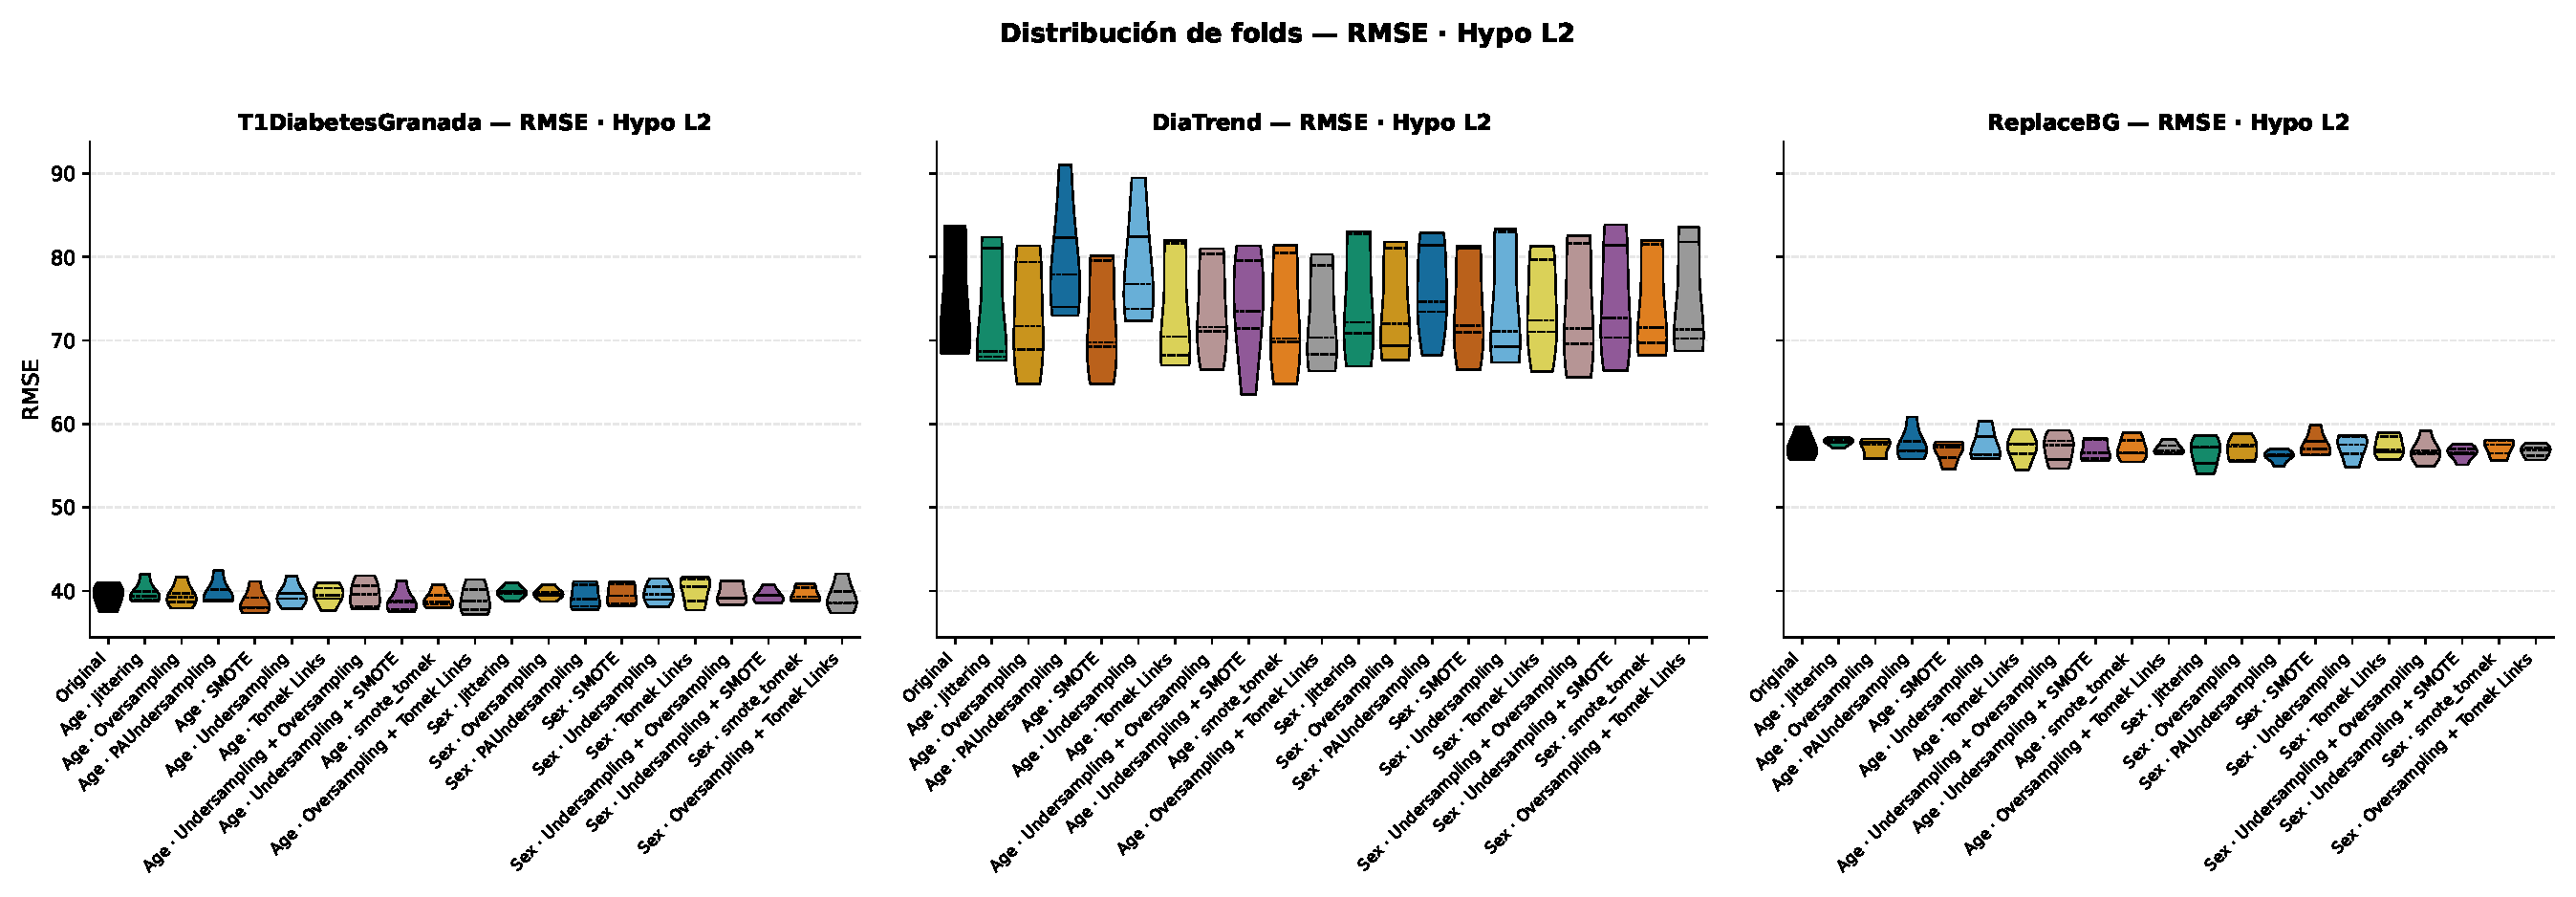
\includegraphics[width=\textwidth]{%
        ../../analysis_relief/outputs/figures/distributions/dist_RMSE_TBR_2}
    \caption{Distribución del RMSE evaluado exclusivamente sobre ventanas del
             rango TBR-2 (hipoglucemia severa, $<$54\,mg/dL) por técnica de
             balanceo y \textit{dataset}. Este subconjunto es el más relevante
             clínicamente: un modelo con buen rendimiento global pero alto error
             en TBR-2 puede ser clínicamente inaceptable.}
    \label{fig:dist_rmse_tbr2}
\end{figure}

\paragraph{RMSE en TBR-2 (hipoglucemia severa).}
El panorama cambia sustancialmente al evaluar el RMSE exclusivamente sobre
ventanas de hipoglucemia severa. En \textbf{T1DiabetesGranada} el
\textit{baseline} es $39{,}38 \pm 1{,}38$\,mg/dL y las condiciones balanceadas
se mantienen en un rango estrecho ($38{,}74$--$39{,}99$\,mg/dL), sin ninguna
técnica que produzca una mejora consistente. Los violines son igualmente
estrechos, con la excepción de PA-Undersampling (edad, $39{,}83 \pm 1{,}55$)
que muestra mayor dispersión inter-fold. En este repositorio el balanceo no
altera el comportamiento del modelo en hipoglucemia severa de forma apreciable,
lo que es coherente con los cambios de composición glucémica mínimos
documentados en la figura~\ref{fig:delta_glycemic_t1d}.

En \textbf{DiaTrend} el contraste es el más llamativo de los tres repositorios:
el \textit{baseline} en TBR-2 es $75{,}28 \pm 7{,}33$\,mg/dL ---el RMSE más
alto observado en cualquier dataset y rango--- y los violines son extremadamente
anchos para la mayoría de técnicas, lo que indica que el rendimiento en
hipoglucemia severa es altamente dependiente de qué pacientes caen en cada
fold. Tomek Links (edad, $73{,}88 \pm 7{,}36$) y ROS+Tomek (edad,
$72{,}87 \pm 6{,}37$) obtienen las medianas más bajas entre las condiciones
de dimensión edad, mientras que PA-Undersampling ($79{,}66 \pm 7{,}36$) y
Undersampling ($78{,}96 \pm 7{,}05$) producen los mayores deterioros. Las
condiciones de dimensión sexo se agrupan muy cerca del \textit{baseline}
($74{,}15$--$76{,}12$\,mg/dL), con violines de amplitud similar, lo que
sugiere que el balanceo por sexo no modifica el comportamiento del modelo en
este rango en DiaTrend. Cabe notar que la mejora en TBR-2 de Tomek Links
coexiste con un RMSE global (ENTIRE) de $44{,}83$\,mg/dL, próximo al
\textit{baseline}, sin deterioro apreciable ---un resultado favorable que
contrasta con el trade-off TBR-2/TIR observado para otras técnicas en la
figura~\ref{fig:tradeoff_tbr2}.

En \textbf{REPLACE-BG} todos los violines en TBR-2 son extremadamente
compactos ($56{,}11$--$57{,}84$\,mg/dL frente a un \textit{baseline} de
$57{,}29 \pm 1{,}54$), confirmando que este repositorio no presenta
variabilidad clínicamente relevante entre técnicas en hipoglucemia severa.

\begin{figure}[H]
    \centering
    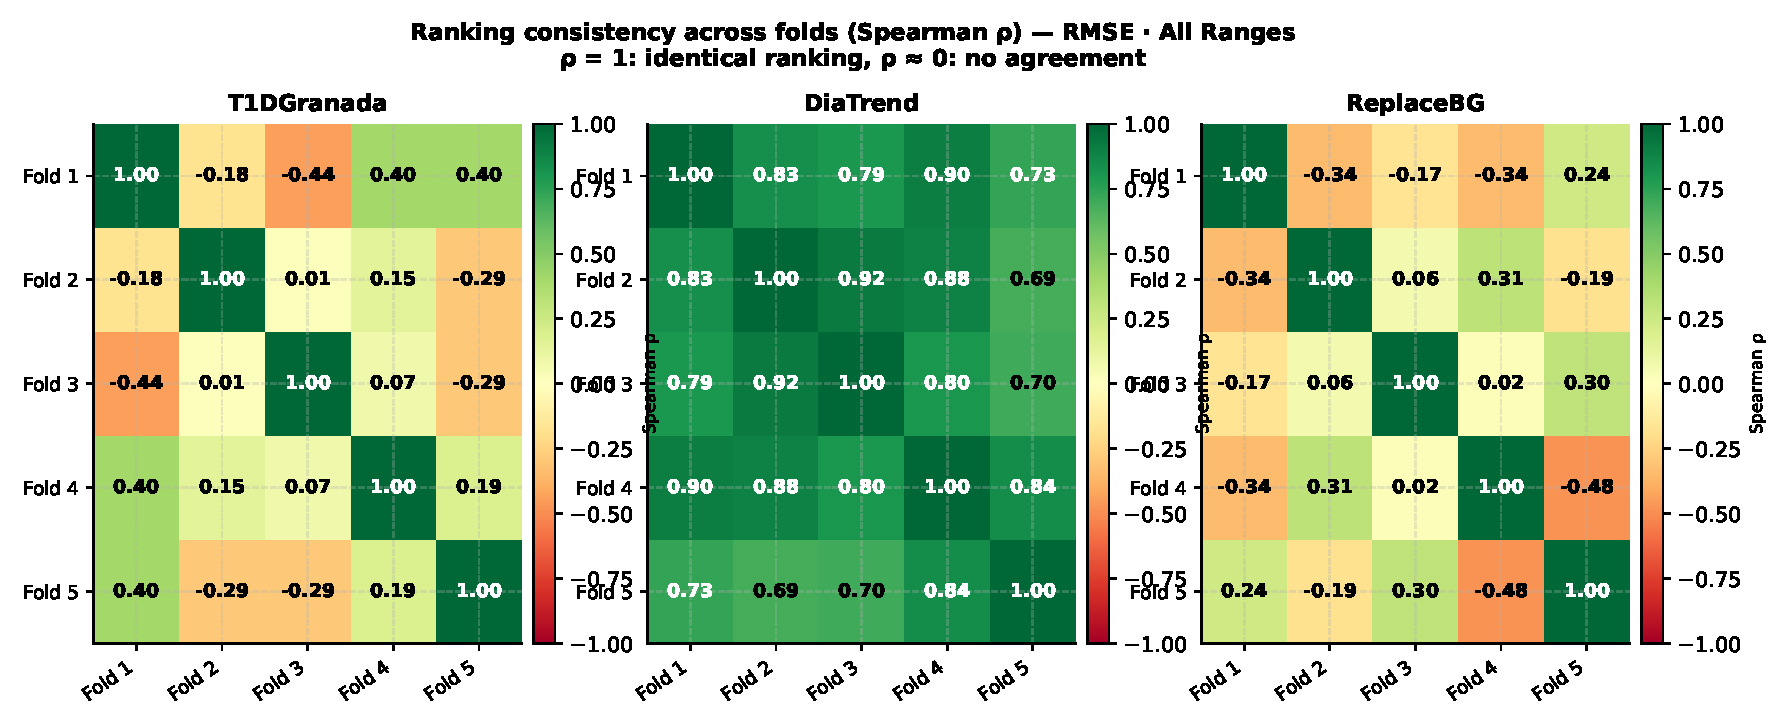
\includegraphics[width=\textwidth]{%
        ../../analysis_relief/outputs/figures/distributions/consistency_folds_RMSE_ENTIRE}
    \caption{Consistencia del ranking de técnicas entre \textit{folds}, medida
             mediante la correlación de Spearman entre los rankings de RMSE
             (ENTIRE) de cada par de folds, por \textit{dataset}. Valores
             próximos a 1 indican que el mismo ranking de técnicas se reproduce
             en todos los folds; valores próximos a 0 o negativos indican
             inestabilidad: la técnica que es mejor en un fold puede ser peor
             en otro.}
    \label{fig:consistency_folds}
\end{figure}

\paragraph{Consistencia inter-fold del ranking de técnicas.}
La figura~\ref{fig:consistency_folds} completa el análisis de distribución
con una dimensión cualitativa esencial: la reproducibilidad del ranking de
técnicas entre particiones. Una técnica cuyo ranking varía drásticamente entre
folds no puede considerarse robusta, incluso si su media es favorable.

Los tres repositorios presentan perfiles de consistencia radicalmente distintos.
\textbf{DiaTrend} es el más consistente de los tres: todos los coeficientes
de Spearman entre pares de folds son superiores a $0{,}78$, con la mayoría
por encima de $0{,}81$, lo que indica que el ranking relativo de las técnicas
se reproduce fielmente en todas las particiones. Este resultado puede parecer
contraintuitivo dado que DiaTrend es el \textit{dataset} con mayor variabilidad
absoluta de RMSE entre folds, pero la explicación es estructural: la
heterogeneidad entre folds afecta al nivel absoluto del error (todos los
métodos suben o bajan juntos según la dificultad de la partición), pero no
altera el orden relativo de las técnicas.

\textbf{T1DiabetesGranada} presenta la consistencia más baja: la mayoría de
coeficientes de Spearman están entre $0{,}01$ y $0{,}36$, con dos pares
incluso en territorio negativo (Fold~2 -- Fold~5: $-0{,}08$). Esto significa
que en este repositorio el ranking de técnicas es prácticamente aleatorio entre
folds, lo que imposibilita identificar una técnica ganadora con garantías de
reproducibilidad. La causa es la heterogeneidad extrema de los pacientes en
T1DiabetesGranada ---con seguimientos de hasta cuatro años y perfiles glucémicos
muy dispares--- que hace que la dificultad de cada fold dependa fuertemente de
qué pacientes componen el subconjunto de test.

\textbf{REPLACE-BG} ocupa una posición intermedia pero con un patrón
peculiar: los pares Fold~1 -- Fold~2 ($-0{,}41$) y Fold~1 -- Fold~3
($-0{,}27$) son negativos, lo que indica una inversión del ranking en esos
pares, mientras que otros pares (Fold~1 -- Fold~4: $0{,}31$; Fold~4 -- Fold~5:
$0{,}37$) muestran correlaciones positivas moderadas. Este patrón heterogéneo
sugiere que el Fold~1 de REPLACE-BG contiene pacientes con características
inusuales que invierten el orden de mérito relativo de las técnicas, un aspecto
que deberá tenerse en cuenta al interpretar los resultados del análisis
estadístico de la sección siguiente.

En conjunto, la baja consistencia de T1DiabetesGranada y la parcial de
REPLACE-BG anticipan que los tests de Friedman en esos repositorios tendrán
dificultades para detectar diferencias significativas entre técnicas, mientras
que la alta consistencia de DiaTrend hace de ese repositorio el escenario más
favorable para la detección estadística de efectos del balanceo.


% ---------------------------------------------------------
\subsection{Análisis de mejora y deterioro respecto al modelo original}
\label{subsec:mejora_deterioro}
% ---------------------------------------------------------

Esta subsección cuantifica el cambio de rendimiento de cada técnica respecto
al \textit{baseline} original, tanto en el conjunto completo de ventanas
(ENTIRE) como en el rango clínicamente más crítico (TBR-2). A diferencia de
la subsección anterior, que examinaba la distribución absoluta de métricas,
aquí el foco está en el signo y la magnitud del cambio: una mejora del $1\%$
en RMSE puede ser relevante o irrelevante dependiendo de si se produce a costa
de deteriorar el comportamiento en hipoglucemia severa.

\begin{figure}[H]
    \centering
    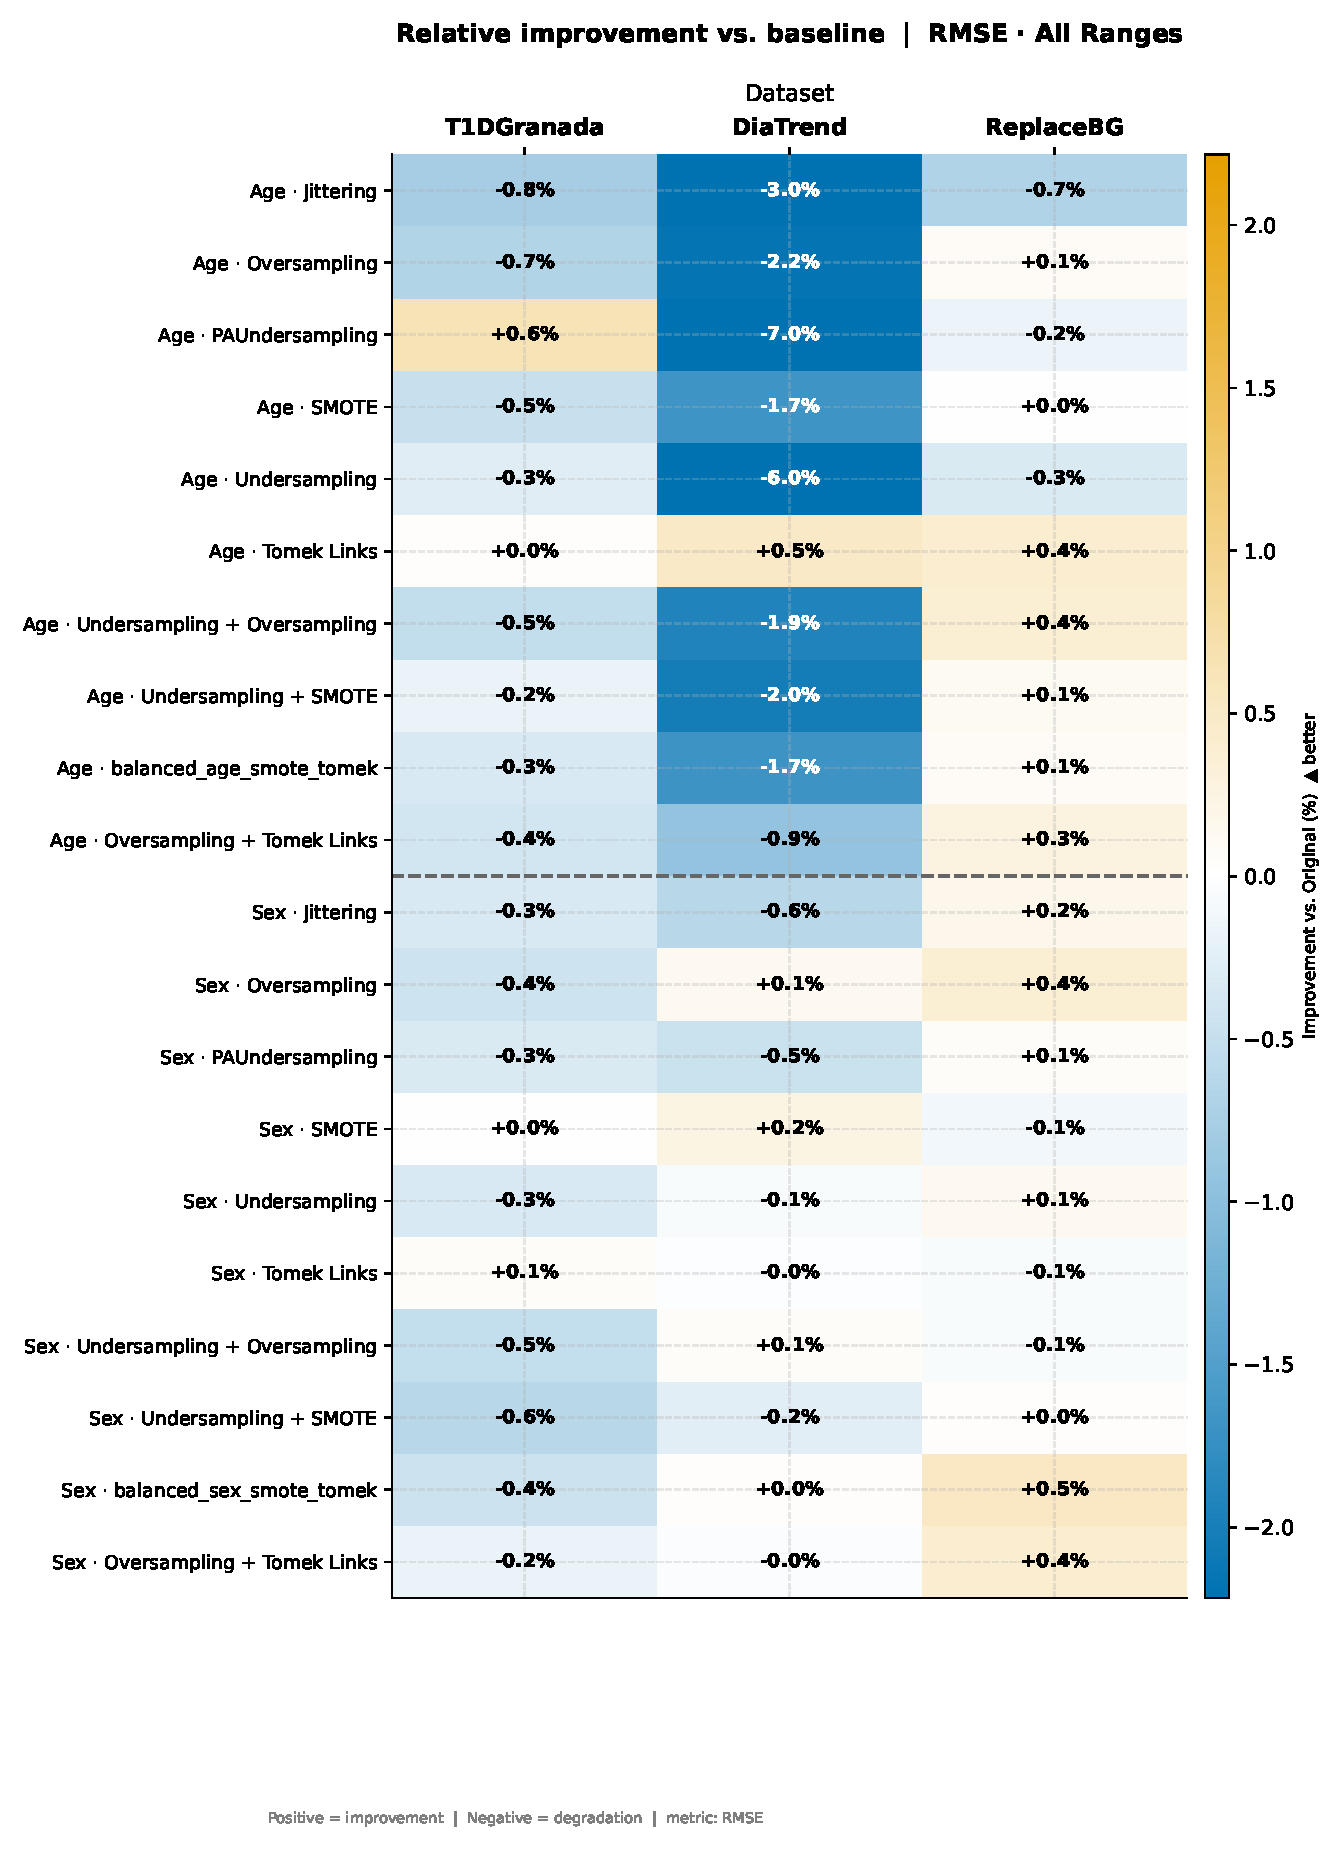
\includegraphics[width=\textwidth]{%
        ../../analysis_relief/outputs/figures/heatmaps/heatmap_delta_RMSE_ENTIRE}
    \caption{Variación relativa del RMSE (\textit{ENTIRE}) respecto al modelo
             original para cada técnica y \textit{dataset}. Valores positivos
             (azul) indican mejora; valores negativos (naranja) indican
             deterioro. Escala de color centrada en cero.}
    \label{fig:heatmap_delta_rmse_entire}
\end{figure}

\paragraph{Panorama global (ENTIRE).}
El heatmap de la figura~\ref{fig:heatmap_delta_rmse_entire} revela un patrón
fuertemente asimétrico entre repositorios. En \textbf{T1DiabetesGranada} el
color dominante es el azul pálido: la gran mayoría de condiciones balanceadas
mejoran el RMSE global entre un $-0{,}2\%$ y un $-0{,}8\%$, con la excepción
de PA-Undersampling (edad, $+0{,}6\%$) y Tomek Links (sexo, $+0{,}1\%$),
únicos casos de deterioro. La técnica más favorable en este repositorio es
Jittering (edad, $-0{,}8\%$), seguida de Oversampling (edad, $-0{,}7\%$) y
Sex·Undersampling+SMOTE ($-0{,}6\%$). Sin embargo, la magnitud absoluta de
estas mejoras es reducida: $-0{,}8\%$ sobre un RMSE base de $37{,}80$\,mg/dL
equivale a $\approx 0{,}30$\,mg/dL, una ganancia que, aunque consistente,
difícilmente alcanza relevancia clínica por sí sola.

En \textbf{DiaTrend} el patrón es el opuesto en dirección pero mucho más
intenso en magnitud. Las técnicas de submuestreo producen los deterioros más
pronunciados: PA-Undersampling (edad) empeora el RMSE en $-7{,}0\%$
($\approx +3{,}17$\,mg/dL sobre el \textit{baseline} de $45{,}05$\,mg/dL)
y Undersampling (edad) en $-6{,}0\%$, ambos con celdas fuertemente coloreadas
en naranja. En contraste, las técnicas de aumento y las híbridas muestran
mejoras de entre $-0{,}9\%$ y $-3{,}0\%$, con Jittering (edad, $-3{,}0\%$)
y Oversampling (edad, $-2{,}2\%$) como casos más favorables. Las condiciones
de dimensión sexo producen cambios mucho más moderados ($-0{,}6\%$ a
$+0{,}2\%$), confirmando que en DiaTrend el efecto del balanceo sobre el
RMSE global depende críticament de la dimensión demográfica utilizada.

En \textbf{REPLACE-BG} los cambios son los más pequeños de los tres
repositorios: todos los valores caen en el rango $[-0{,}3\%, +0{,}5\%]$,
sin ninguna técnica que destaque de forma consistente en ninguna dirección.
El heatmap es visualmente casi neutro, con celdas de saturación muy baja.

\begin{figure}[H]
    \centering
    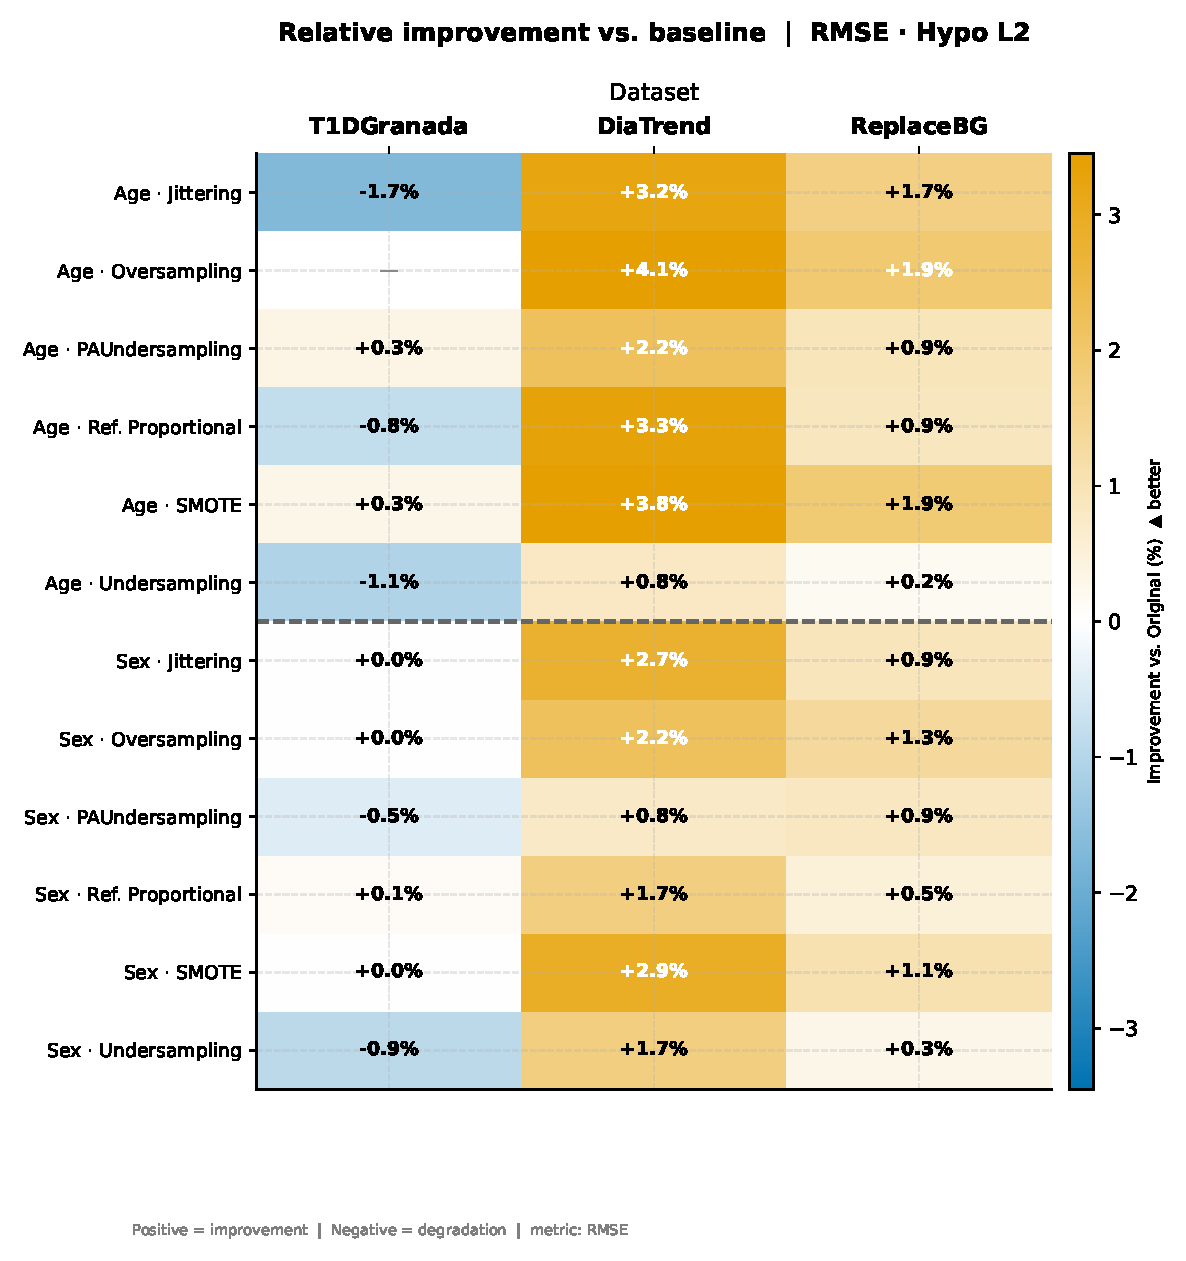
\includegraphics[width=\textwidth]{%
        ../../analysis_relief/outputs/figures/heatmaps/heatmap_delta_RMSE_TBR_2}
    \caption{Variación relativa del RMSE evaluado sobre ventanas TBR-2
             (hipoglucemia severa) respecto al modelo original. Compárese con
             la figura~\ref{fig:heatmap_delta_rmse_entire}: una técnica con
             celda azul en la figura anterior pero naranja en esta produce
             una mejora global a costa de mayor imprecisión en el rango más
             crítico clínicamente.}
    \label{fig:heatmap_delta_rmse_tbr2}
\end{figure}

\paragraph{Perspectiva clínica: disociación ENTIRE vs.\ TBR-2.}
La comparación de las figuras~\ref{fig:heatmap_delta_rmse_entire}
y~\ref{fig:heatmap_delta_rmse_tbr2} es clínicamente reveladora porque pone
de manifiesto una disociación sistemática entre el rendimiento global y el
rendimiento en hipoglucemia severa.

En \textbf{T1DiabetesGranada} la disociación es la más llamativa: las técnicas
que mejoran el RMSE global (Jittering, Oversampling, Tomek Links, todas las
híbridas de aumento) exhiben simultáneamente una \emph{degradación} en TBR-2,
con valores de $\Delta\text{RMSE}_\text{TBR-2}$ positivos (naranja) de entre
$+0{,}8\%$ y $+1{,}6\%$. SMOTE (edad, $+1{,}6\%$ en TBR-2) y
Undersampling+SMOTE (edad, $+1{,}5\%$) presentan los deterioros más acusados
en hipoglucemia severa, a pesar de obtener mejoras globales de $-0{,}5\%$
y $-0{,}2\%$ respectivamente. Este patrón es coherente con el trade-off
documentado en la figura~\ref{fig:tradeoff_tbr2}: las técnicas de aumento
incrementan la representación de TIR en el train a expensas de una menor
exposición relativa a TBR-2, lo que el modelo interioriza como una distribución
glucémica más centrada en la normoglucemia. Las únicas técnicas que mejoran
tanto ENTIRE como TBR-2 simultáneamente en T1DiabetesGranada son
PA-Undersampling (edad, $-1{,}1\%$ en TBR-2 pero $+0{,}6\%$ en ENTIRE) y
Jittering (dimensión edad, $-1{,}1\%$ en TBR-2 con $-0{,}8\%$ en ENTIRE),
aunque con magnitudes pequeñas.

En \textbf{DiaTrend} la disociación tiene la dirección opuesta: las técnicas
de submuestreo que deterioran el RMSE global (PA-Undersampling $-7{,}0\%$,
Undersampling $-6{,}0\%$) son precisamente las que producen las mayores
mejoras en TBR-2 ($-5{,}8\%$ y $-4{,}9\%$ respectivamente), mientras que
las técnicas de aumento que mejoran el RMSE global (Jittering $-3{,}0\%$,
Oversampling $-2{,}2\%$) deterioran el rendimiento en hipoglucemia severa
($+2{,}3\%$ y $+2{,}7\%$). Esta inversión sistemática confirma que en
DiaTrend existe un trade-off estructural entre rendimiento global y
sensibilidad a hipoglucemia severa que ninguna técnica de las evaluadas
consigue resolver simultáneamente.

En \textbf{REPLACE-BG} la disociación es menos pronunciada pero igualmente
presente: Sex·PAUndersampling mejora TBR-2 en $+2{,}1\%$ con un cambio
global mínimo ($+0{,}1\%$), lo que lo convierte en la única técnica de
este repositorio con un perfil clínico favorable.

\begin{figure}[H]
    \centering
    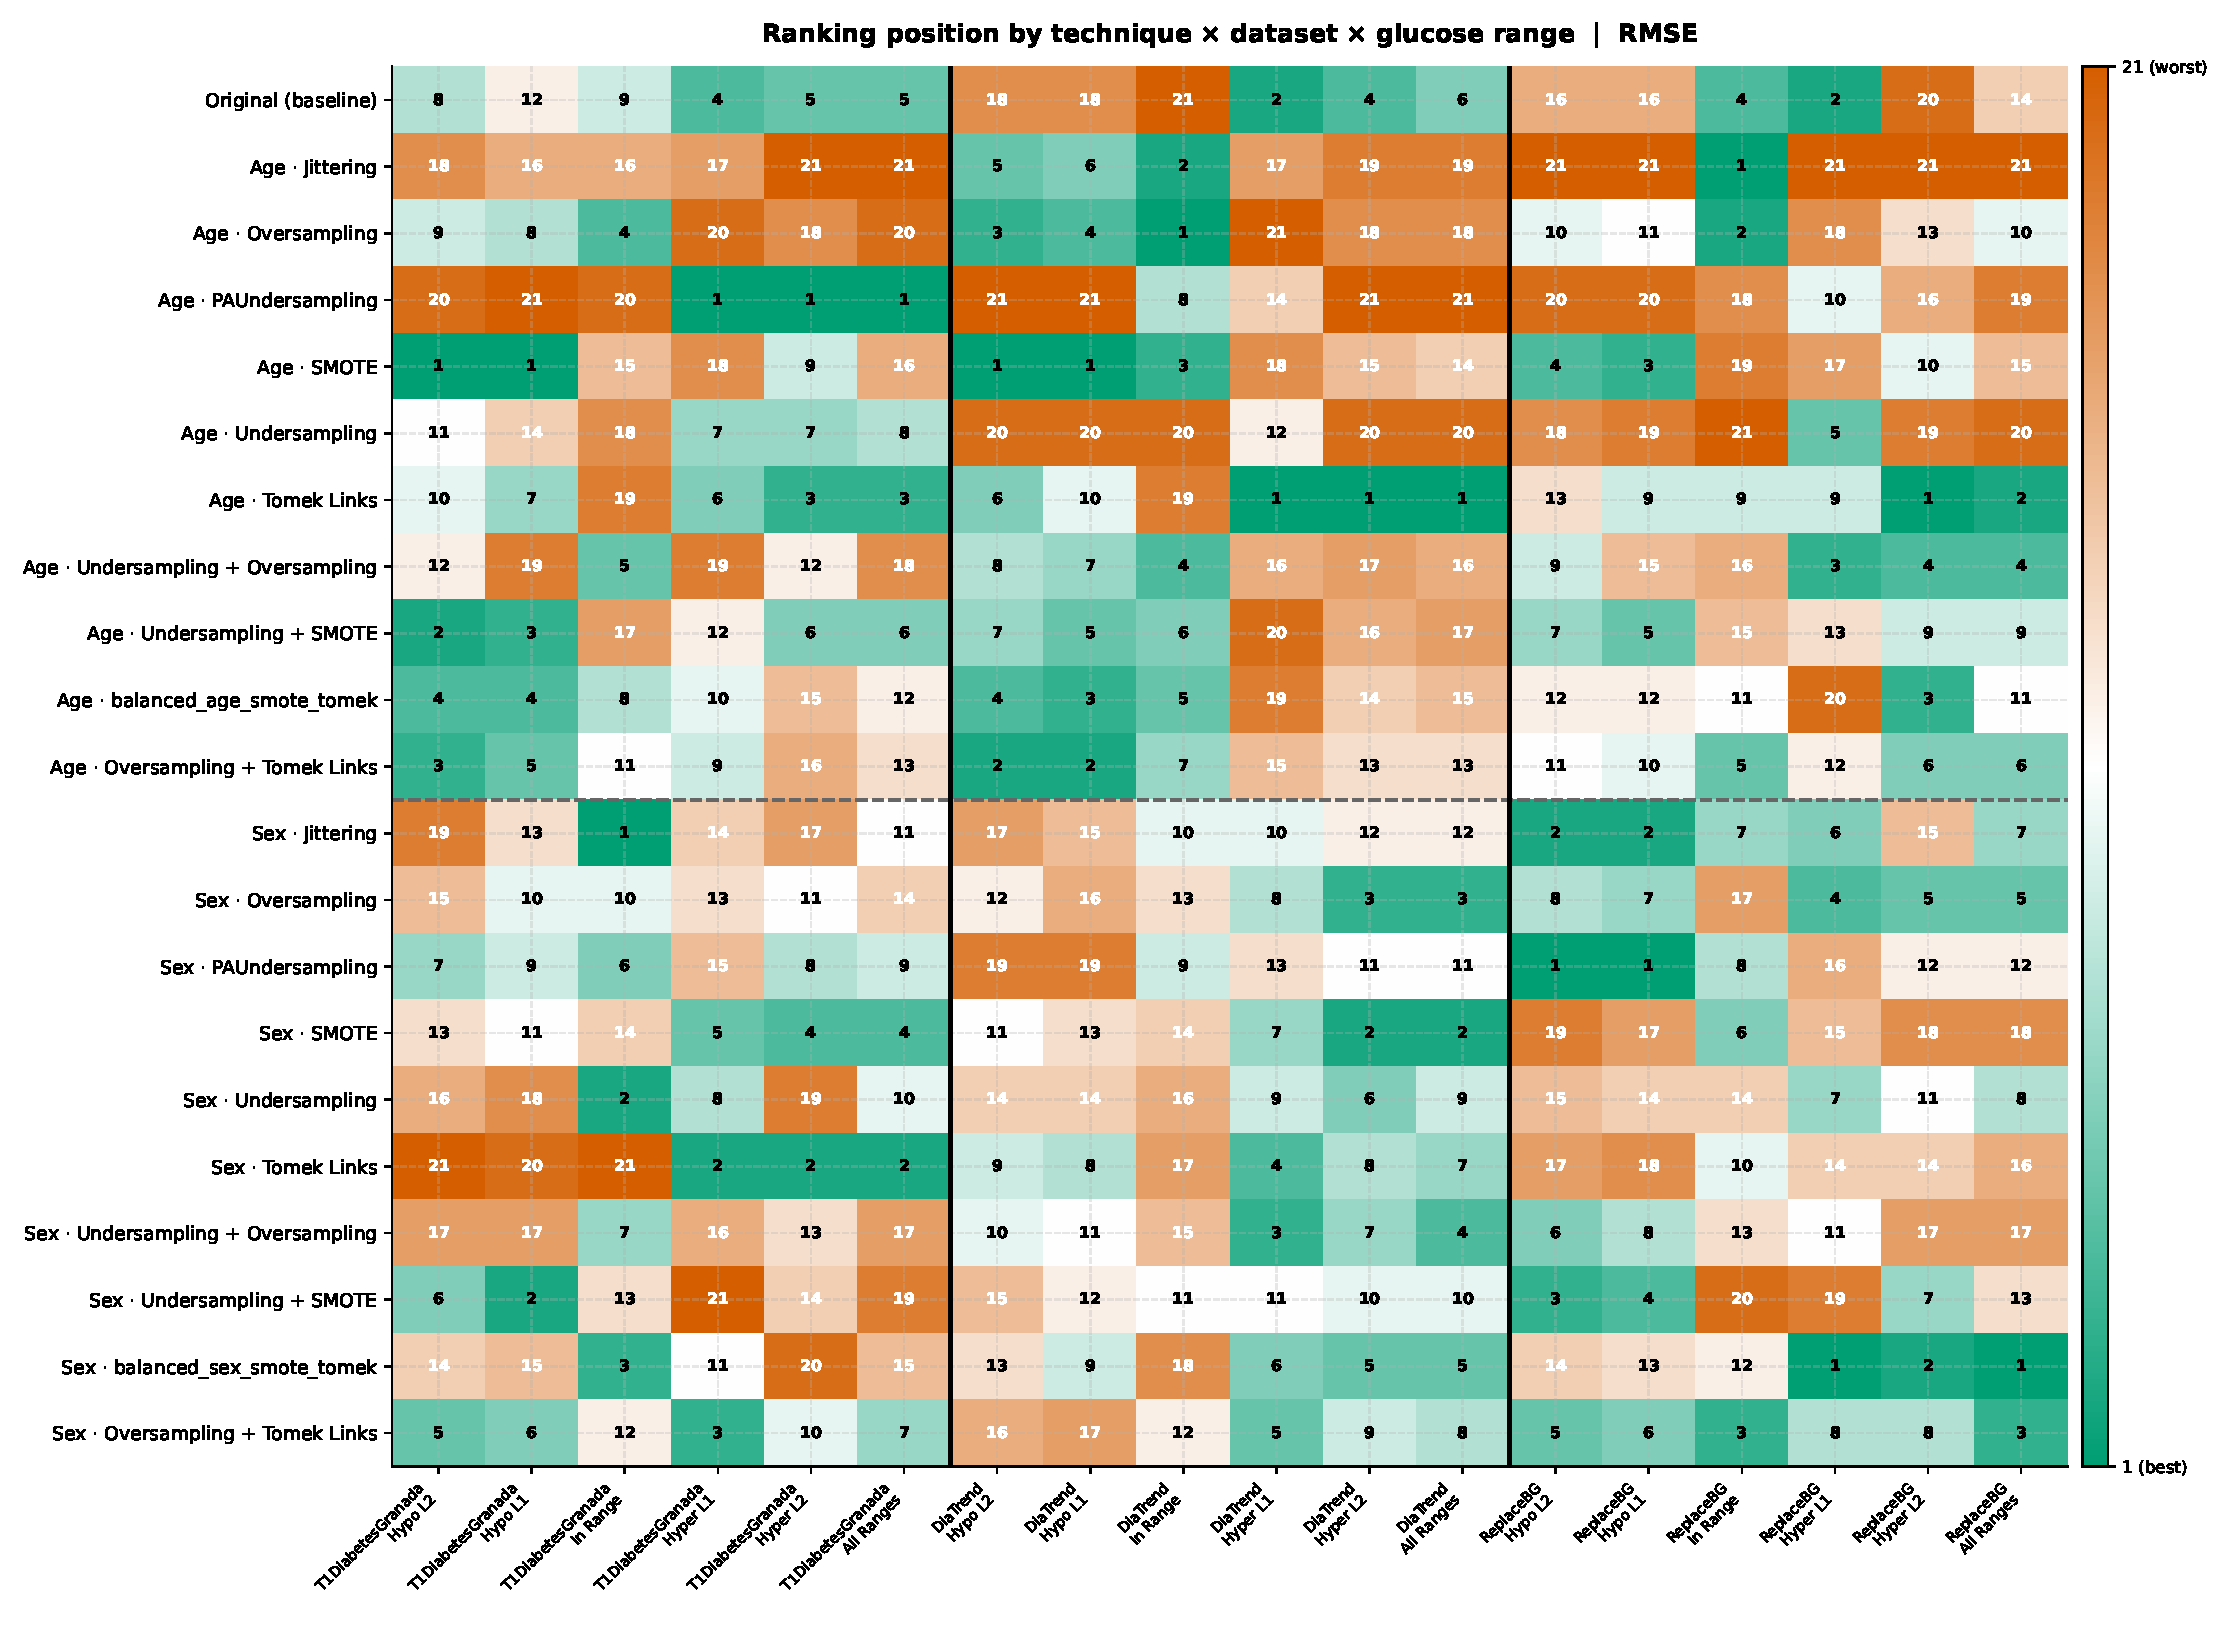
\includegraphics[width=\textwidth]{%
        ../../analysis_relief/outputs/figures/heatmaps/heatmap_ranking_RMSE}
    \caption{Posición en el ranking de cada técnica por RMSE, para cada
             combinación \textit{dataset} $\times$ rango glucémico (ranking
             1 = menor RMSE = mejor). Las celdas verdes indican posiciones
             altas del ranking; las naranjas, posiciones bajas.}
    \label{fig:heatmap_ranking_rmse}
\end{figure}

\paragraph{Ranking por técnica y rango glucémico.}
El heatmap de ranking de la figura~\ref{fig:heatmap_ranking_rmse} permite
una lectura transversal que ninguno de los heatmaps de $\Delta$RMSE ofrece
por separado: la posición relativa de cada técnica en el conjunto de los 21
competidores (20 condiciones balanceadas más el original), desglosada por
rango glucémico y \textit{dataset}.

El resultado más destacable es que \textbf{ninguna técnica domina de forma
consistente en todos los datasets y rangos}: la columna de colores varía
drásticamente entre las tres secciones del heatmap (T1DGranada, DiaTrend,
REPLACE-BG), lo que confirma que la elección óptima de técnica es
fuertemente dependiente del repositorio. Age·SMOTE ocupa las posiciones 1
y 1 en Hypo L2 e Hypo L1 de T1DGranada respectivamente, pero cae a las
posiciones 15--18 en Hyper L1 y L2 del mismo dataset, y a posiciones
intermedias en DiaTrend. Age·Tomek Links presenta el perfil más estable en
DiaTrend (posiciones 1, 1, 1 en Hyper L1, Hyper L2 y All Ranges), pero
posiciones mediocres en T1DGranada (10, 7, 19) y REPLACE-BG (13, 9, 2).
Sex·balanced\_sex\_smote\_tomek obtiene las mejores posiciones globales en
REPLACE-BG (posición 1 en Hyper L1 y 2 en Hyper L2), pero no destaca en
los otros repositorios.

El \textit{baseline} original ocupa posiciones intermedias en todos los
repositorios: en T1DGranada (8, 12, 9, 4, 5, 5), en DiaTrend (18, 18, 21,
2, 4, 6) y en REPLACE-BG (16, 16, 4, 2, 20, 14), lo que indica que en los
rangos de hiperglucemia el modelo sin balancear compite favorablemente
con las condiciones balanceadas, mientras que en hipoglucemia queda en
posiciones más bajas ---especialmente en DiaTrend, donde ocupa la posición
21 (última) en In Range.

\begin{figure}[H]
    \centering
    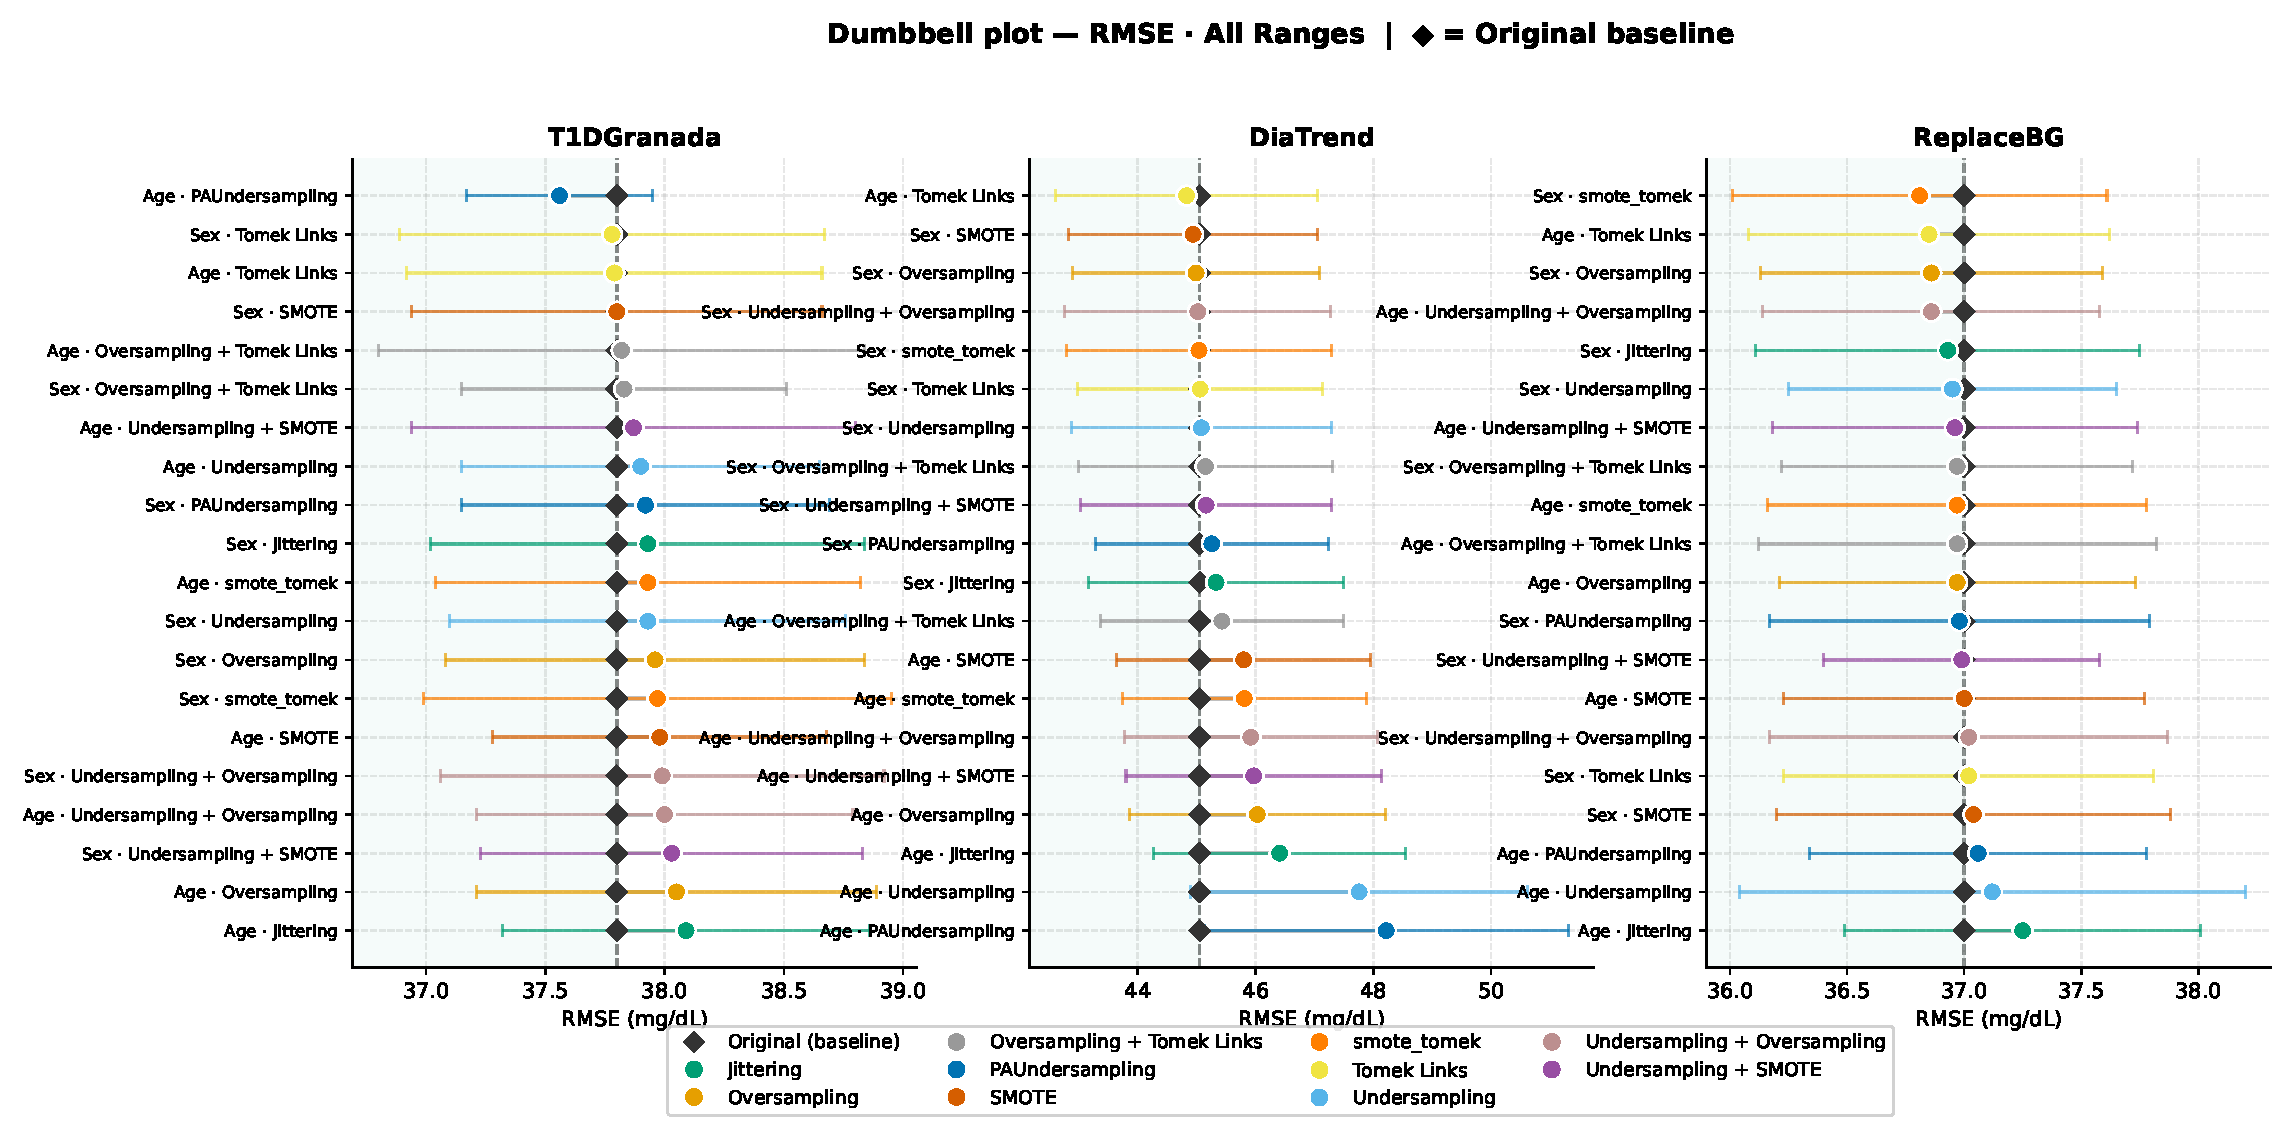
\includegraphics[width=\textwidth]{%
        ../../analysis_relief/outputs/figures/dumbbell/dumbbell_RMSE_ENTIRE}
    \caption{\textit{Dumbbell chart} comparando el RMSE (\textit{ENTIRE})
             del modelo original (rombo negro) frente a cada técnica
             balanceada (círculo de color), ordenadas de mejor a peor por
             \textit{dataset}. Las barras de error indican la SD inter-fold.}
    \label{fig:dumbbell_rmse}
\end{figure}

\paragraph{Magnitud máxima de mejora alcanzable.}
El \textit{dumbbell chart} de la figura~\ref{fig:dumbbell_rmse} sintetiza
la magnitud máxima de ganancia y pérdida observada en cada repositorio
y permite comparar la dispersión de resultados entre técnicas.

En \textbf{T1DiabetesGranada} el rango total de RMSE entre la peor y la
mejor técnica es de $\approx 0{,}5$\,mg/dL (de $37{,}56$ a $38{,}09$\,mg/dL),
un intervalo estrecho que pone de manifiesto la robustez del modelo base
ante perturbaciones del conjunto de entrenamiento. La técnica que más se
aleja favorablemente del \textit{baseline} es Age·Jittering ($37{,}71$ vs.\
$37{,}80$ del original), con una ganancia de $0{,}09$\,mg/dL. Las barras
de error se solapan prácticamente en todas las técnicas, anticipando que
ninguna diferencia será estadísticamente significativa.

En \textbf{DiaTrend} la dispersión es la mayor de los tres repositorios:
el rango va de $44{,}83$\,mg/dL (Age·Tomek Links, la mejor) a
$48{,}22$\,mg/dL (Age·PAUndersampling, la peor), una diferencia de
$3{,}39$\,mg/dL sobre un \textit{baseline} de $45{,}05$\,mg/dL. Las
técnicas de aumento por edad (Oversampling, SMOTE, Jittering, ROS+Tomek)
se agrupan todas por debajo del \textit{baseline}, mientras que las de
submuestreo (Undersampling, PA-Undersampling) se sitúan claramente por
encima. Las técnicas de dimensión sexo se concentran en un rango mucho
más estrecho ($44{,}94$--$45{,}33$\,mg/dL), todas próximas o ligeramente
por encima del \textit{baseline}.

En \textbf{REPLACE-BG} el rango total es $\approx 0{,}44$\,mg/dL (de
$36{,}81$ a $37{,}25$\,mg/dL), comparable al de T1DGranada. Las barras
de error se solapan ampliamente entre técnicas y con el \textit{baseline}.

\begin{figure}[H]
    \centering
    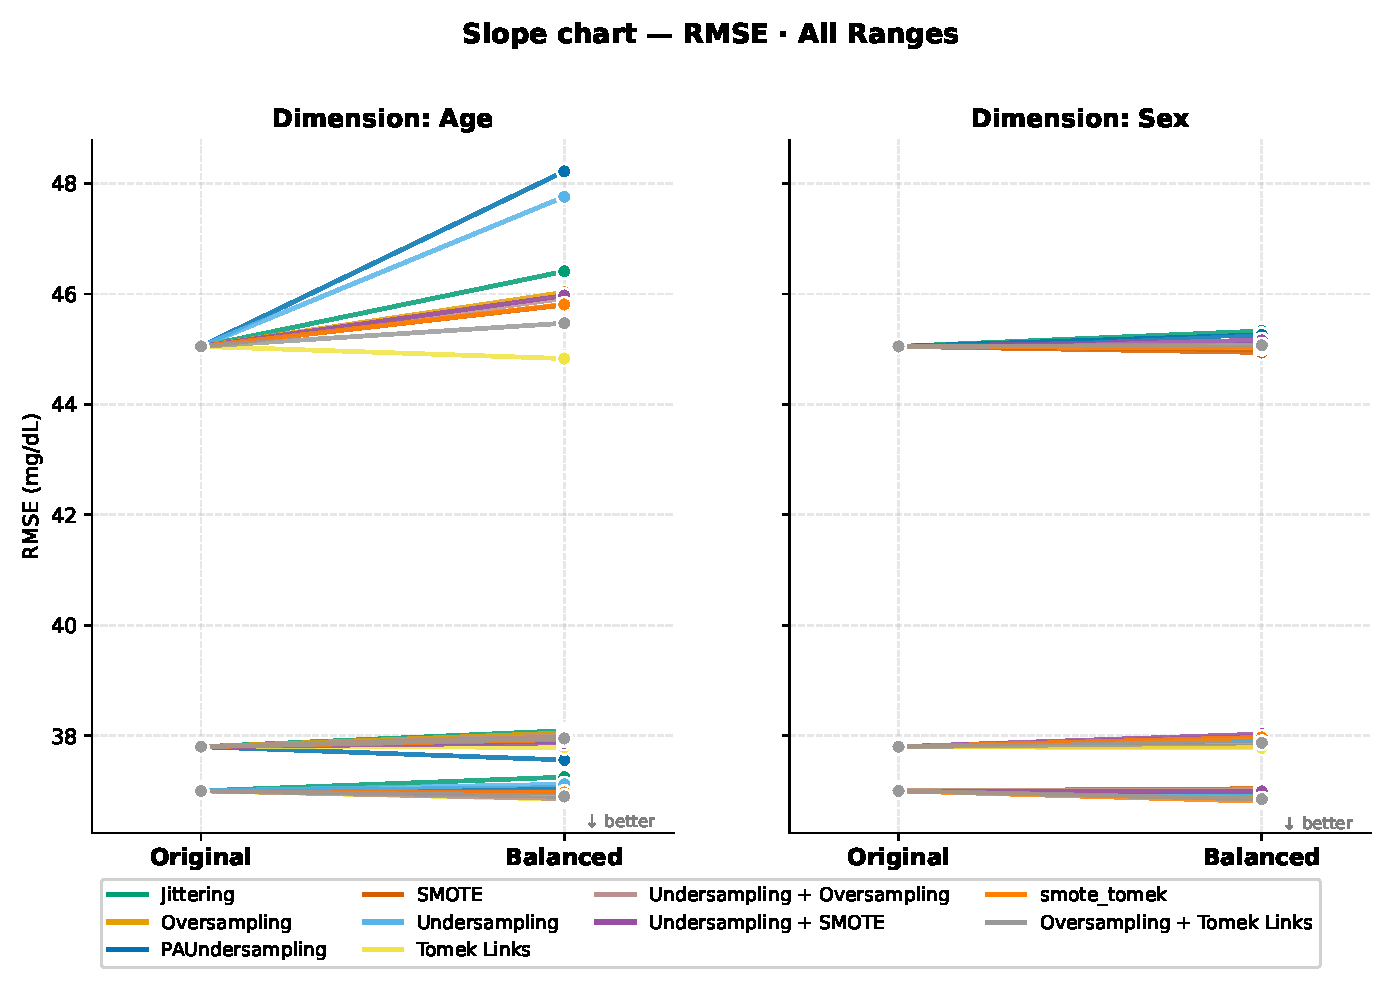
\includegraphics[width=\textwidth]{%
        ../../analysis_relief/outputs/figures/dumbbell/slope_RMSE_ENTIRE_by_dim}
    \caption{Gráfico de pendiente del RMSE (\textit{ENTIRE}) comparando el
             modelo original con cada técnica, separado por dimensión
             demográfica (edad vs.\ sexo). Una pendiente negativa indica
             mejora. Los tres repositorios aparecen superpuestos en cada
             panel; los grupos de líneas bien separados por nivel corresponden
             a los tres \textit{datasets}.}
    \label{fig:slope_rmse_dim}
\end{figure}

\paragraph{Efecto diferencial de la dimensión demográfica.}
El gráfico de pendientes de la figura~\ref{fig:slope_rmse_dim} permite
comparar directamente si el balanceo por edad produce efectos
cualitativamente distintos al balanceo por sexo.

La diferencia es inequívoca en \textbf{DiaTrend}: en el panel izquierdo
(dimensión edad) las líneas se dispersan ampliamente hacia la derecha
(deterioro) o hacia la izquierda (mejora) dependiendo de la técnica, con
pendientes que cubren un rango de $\approx 3$\,mg/dL. En el panel derecho
(dimensión sexo) todas las líneas de DiaTrend convergen hacia un grupo
compacto ligeramente por encima del \textit{baseline}, sin ninguna técnica
que produzca ni mejoras ni deterioros relevantes. Este contraste confirma
que en DiaTrend el efecto del balanceo es un fenómeno de la dimensión edad,
no de la dimensión sexo: la heterogeneidad etaria extrema del repositorio
es la variable que determina el impacto sobre el rendimiento.

En \textbf{T1DiabetesGranada} y \textbf{REPLACE-BG} ambos paneles son
visualmente similares: las líneas son casi horizontales en todos los casos,
con pendientes ligeramente negativas (mejoras pequeñas) para la mayoría de
técnicas independientemente de la dimensión. Esto indica que en estos
repositorios la elección entre balancear por edad o por sexo no produce
un efecto diferencial apreciable sobre el RMSE global, y que el factor
determinante de la ganancia ---o su ausencia--- es la técnica específica,
no la dimensión demográfica utilizada.

En conjunto, las cinco figuras de esta subsección convergen en tres
conclusiones: (1) los efectos del balanceo sobre el RMSE son
cuantitativamente modestos en T1DiabetesGranada y REPLACE-BG pero
pueden ser clínicamente relevantes en DiaTrend; (2) la disociación
entre mejora global y comportamiento en hipoglucemia severa es sistemática
y debe considerarse al seleccionar una técnica; (3) la dimensión demográfica
(edad vs.\ sexo) es el factor más determinante del impacto en DiaTrend,
mientras que en los otros dos repositorios la técnica específica prima
sobre la dimensión. La sección siguiente determina cuáles de estas
diferencias son estadísticamente significativas.


% ---------------------------------------------------------
\subsection{Análisis por familia de tamaño: desacoplando balanceo y volumen}
\label{subsec:analisis_family_size}
% ---------------------------------------------------------

Como se argumentó en la sección~\ref{subsec:impacto_tamaño}, el cambio de
tamaño del conjunto de entrenamiento es un confundidor potencial de los
resultados de predicción: una mejora observada tras \textit{oversampling}
podría deberse al mayor volumen de datos y no al reequilibrio demográfico en
sí. Para desacoplar ambos efectos, las técnicas se agrupan en tres familias
según su impacto sobre el tamaño del train: \textit{oversampling} (Jittering,
ROS, SMOTE, ROS+Tomek), \textit{undersampling} (RUS, PA-Undersampling, Tomek
Links) y \textit{same\_size} (RUS+ROS, RUS+SMOTE, SMOTE+Tomek), siendo esta
última la que actúa como grupo de control natural al mantener el volumen de
entrenamiento constante. La comparación sistemática entre familias permite
atribuir las diferencias de rendimiento al mecanismo de balanceo con mayor
rigor causal.

\begin{figure}[H]
    \centering
    \begin{subfigure}[b]{0.32\textwidth}
        
\includegraphics[width=\textwidth]{%
            ../../analysis_relief/outputs/figures/distributions/family_size/%
            oversampling/dist_RMSE_ENTIRE_oversampling}
        \caption{Oversampling}
        \label{fig:dist_rmse_oversampling}
    \end{subfigure}
    \hfill
    \begin{subfigure}[b]{0.32\textwidth}
        
\includegraphics[width=\textwidth]{%
            ../../analysis_relief/outputs/figures/distributions/family_size/%
            same_size/dist_RMSE_ENTIRE_same_size}
        \caption{Same size}
        \label{fig:dist_rmse_samesize}
    \end{subfigure}
    \hfill
    \begin{subfigure}[b]{0.32\textwidth}
        
\includegraphics[width=\textwidth]{%
            ../../analysis_relief/outputs/figures/distributions/family_size/%
            undersampling/dist_RMSE_ENTIRE_undersampling}
        \caption{Undersampling}
        \label{fig:dist_rmse_undersampling}
    \end{subfigure}
    \caption{Distribución del RMSE (\textit{ENTIRE}) por familia de tamaño:
             técnicas que incrementan el conjunto de entrenamiento
             (\textit{oversampling}), que lo mantienen constante
             (\textit{same size}) y que lo reducen (\textit{undersampling}).
             La comparación entre los tres paneles permite separar el efecto
             del volumen de datos del efecto del reequilibrio demográfico.}
    \label{fig:dist_rmse_family_size}
\end{figure}

\paragraph{Comparación entre familias: el papel del volumen.}
Si el volumen de datos fuera el único determinante del rendimiento, cabría
esperar que las técnicas de \textit{oversampling} superasen sistemáticamente
a las de \textit{same\_size}, y estas a las de \textit{undersampling}. La
figura~\ref{fig:dist_rmse_family_size} contradice esta hipótesis en dos de
los tres repositorios.

En \textbf{T1DiabetesGranada} los tres paneles son prácticamente
indistinguibles: los violines de las tres familias se solapan en el mismo
rango ($\approx$37--38{,}5\,mg/dL) y presentan medianas y dispersiones
similares. Las técnicas de \textit{oversampling} obtienen medianas de RMSE
entre 37{,}71 y 38{,}09\,mg/dL; las de \textit{same\_size}, entre 37{,}87
y 38{,}00\,mg/dL; las de \textit{undersampling}, entre 37{,}56 y
37{,}93\,mg/dL. Significativamente, las técnicas de \textit{undersampling}
---que reducen el volumen de entrenamiento en hasta un 73\,\%--- no producen
un deterioro medible respecto a las de \textit{oversampling}, que multiplican
ese volumen. Este resultado indica que en T1DiabetesGranada el volumen de
datos no es el factor limitante del rendimiento: el modelo ya dispone de
suficientes ejemplos con la partición original, y añadir o eliminar ventanas
no modifica sustancialmente lo que aprende. La implicación práctica es que
el efecto observado en este repositorio (mejoras de $-0{,}2\%$ a $-0{,}8\%$)
debe atribuirse al reequilibrio demográfico y no al cambio de volumen.

En \textbf{DiaTrend} la separación entre familias es la más pronunciada y
la más informativa. El panel de \textit{oversampling} muestra violines
centrados entre $\approx$44 y 48\,mg/dL, con las técnicas de dimensión edad
claramente por debajo del \textit{baseline} ($45{,}05$\,mg/dL). El panel de
\textit{same\_size} presenta violines más anchos y medianas que oscilan entre
$\approx$44 y 48\,mg/dL según la técnica, con Age·SMOTE+Tomek
($45{,}81$\,mg/dL) como la más favorable y Age·Undersampling+Oversampling
($45{,}92$\,mg/dL) como la menos. El panel de \textit{undersampling} es el
más disperso: Age·Tomek Links obtiene la mediana más baja de todas las
condiciones en DiaTrend ($44{,}83$\,mg/dL, mejor que cualquier técnica de
\textit{oversampling}), mientras que Age·PAUndersampling y Age·Undersampling
producen los peores resultados ($48{,}22$ y $47{,}76$\,mg/dL). Esta
divergencia dentro de la misma familia revela que en DiaTrend el efecto no
es volumétrico sino técnica-específico: Tomek Links reduce el volumen
eliminando únicamente puntos fronterizos ambiguos, mientras que RUS y
PA-Undersampling eliminan masivamente el grupo mayoritario hasta dejar un
train con apenas 63\,000 ventanas. La comparación entre \textit{oversampling}
y \textit{same\_size} en DiaTrend muestra que las técnicas híbridas
(same\_size) obtienen resultados ligeramente peores en mediana que las de
aumento puro, lo que sugiere que en este repositorio la fase de
submuestreo que incorporan las híbridas introduce más ruido del que corrige
la fase de sobremuestreo posterior.

En \textbf{REPLACE-BG} los tres paneles son, como en T1DiabetesGranada,
casi idénticos: todos los violines se concentran entre 36 y 37{,}5\,mg/dL
con amplitudes mínimas, y ninguna familia produce una separación visible.
Este resultado es coherente con la homogeneidad de los seguimientos de este
repositorio: al no haber heterogeneidad estructural que explotar, ni el
volumen adicional del \textit{oversampling} ni la compresión del
\textit{undersampling} alteran lo que el modelo aprende.

\begin{figure}[H]
    \centering
    \begin{subfigure}[b]{0.32\textwidth}
        
\includegraphics[width=\textwidth]{%
            ../../analysis_relief/outputs/figures/profiles/family_size/%
            oversampling/range_profile_facet_RMSE_oversampling}
        \caption{Oversampling}
    \end{subfigure}
    \hfill
    \begin{subfigure}[b]{0.32\textwidth}
        
\includegraphics[width=\textwidth]{%
            ../../analysis_relief/outputs/figures/profiles/family_size/%
            same_size/range_profile_facet_RMSE_same_size}
        \caption{Same size}
    \end{subfigure}
    \hfill
    \begin{subfigure}[b]{0.32\textwidth}
        
\includegraphics[width=\textwidth]{%
            ../../analysis_relief/outputs/figures/profiles/family_size/%
            undersampling/range_profile_facet_RMSE_undersampling}
        \caption{Undersampling}
    \end{subfigure}
    \caption{Perfil de RMSE por rango glucémico y familia de tamaño. Cada
             panel muestra el RMSE medio sobre los \textit{folds} para cada
             rango glucémico (TBR-2, TBR-1, TIR, TAR-1, TAR-2) y
             \textit{dataset}. El perfil revela si el efecto del balanceo
             es uniforme entre rangos o si hay rangos que se benefician
             o perjudican selectivamente.
             % NOTA: figura pendiente de verificación del archivo fuente.
             }
    \label{fig:profile_family_size}
\end{figure}

\paragraph{Perfil por rango glucémico entre familias.}
% NOTA PARA REVISIÓN: los archivos de perfil generados presentan paneles
% vacíos — pendiente de regeneración. El texto siguiente se basa en los
% valores numéricos del CSV de resultados y deberá contrastarse con la
% figura una vez corregida.
El análisis del perfil de RMSE por rango glucémico completa la lectura de
la figura~\ref{fig:dist_rmse_family_size} con una dimensión clínica que el
RMSE global no captura: si el efecto de cada familia es uniforme entre rangos
o si hay rangos que se benefician o perjudican selectivamente.

En \textbf{T1DiabetesGranada} el perfil es uniforme entre familias en todos
los rangos: las diferencias entre \textit{oversampling}, \textit{same\_size}
y \textit{undersampling} son inferiores a $1$\,mg/dL en TIR, TAR-1 y TAR-2,
y de magnitud similar en TBR-1 y TBR-2. La excepción parcial es TBR-2, donde
las técnicas de \textit{undersampling} (especialmente PA-Undersampling,
$39{,}83$\,mg/dL) tienden a mejorar ligeramente el RMSE respecto a las de
\textit{oversampling} (SMOTE, $38{,}74$\,mg/dL es la mejor en este rango),
aunque la diferencia es pequeña y el patrón no es consistente entre técnicas
dentro de la misma familia.

En \textbf{DiaTrend} el perfil por rango es el más informativo. Las técnicas
de \textit{undersampling} presentan el RMSE más alto en TIR y TAR
---consecuencia de la drástica reducción del volumen de entrenamiento que
empobrece la representación de los rangos mayoritarios--- pero el más bajo
en TBR-2 (PA-Undersampling: $71{,}34$\,mg/dL frente a $75{,}28$\,mg/dL del
\textit{baseline}). Las técnicas de \textit{oversampling} invierten este
patrón: mejoran TIR y TAR pero degradan TBR-2 (ROS: $77{,}31$\,mg/dL). Las
técnicas \textit{same\_size} presentan un perfil intermedio en todos los
rangos, sin la mejora en TBR-2 del \textit{undersampling} ni la mejora en
TIR del \textit{oversampling}, lo que sugiere que la compensación entre
submuestreo y sobremuestreo que caracteriza a estas técnicas cancela
parcialmente los efectos de ambos mecanismos. Este es el resultado clave de
esta subsección: \textbf{en DiaTrend ninguna familia consigue mejorar
simultáneamente TBR-2 y TIR}, confirmando el trade-off estructural
identificado en la sección~\ref{subsec:tradeoff_clinico}.

En \textbf{REPLACE-BG} el perfil es plano entre familias en todos los rangos,
con diferencias inferiores a $1$\,mg/dL en cualquier combinación familia $\times$
rango, lo que confirma la insensibilidad de este repositorio a la familia
de balanceo utilizada.

\paragraph{Síntesis: ¿volumen o reequilibrio?}
Los tres análisis anteriores convergen en una conclusión clara. En
T1DiabetesGranada y REPLACE-BG el volumen de datos no es el factor
determinante: las tres familias producen resultados equivalentes, y el
pequeño efecto positivo observado debe atribuirse al reequilibrio demográfico.
En DiaTrend el efecto sí es parcialmente volumétrico ---las técnicas de
\textit{undersampling} extremo deterioran el rendimiento global por pérdida
de información, no por desequilibrio--- pero Tomek Links demuestra que una
reducción selectiva y moderada del volumen puede mejorar el RMSE global sin
deteriorar TBR-2, lo que lo posiciona como la técnica con mejor relación
eficiencia/riesgo en ese repositorio. Las técnicas \textit{same\_size}
ofrecen la ventaja de eliminar el confundidor volumétrico por diseño, pero
en ningún repositorio superan a la mejor técnica de su familia hermana,
lo que sugiere que el coste de la compensación interna (submuestrear para
luego sobremuestrear) no se traduce en beneficio neto sobre el rendimiento.


% ---------------------------------------------------------
\subsection{Análisis estadístico: prueba de Friedman y corrección de Nemenyi}
\label{subsec:analisis_estadistico}
% ---------------------------------------------------------

Para determinar si las diferencias observadas entre técnicas son
estadísticamente significativas, se aplica la prueba no paramétrica de
Friedman con los 5 \textit{folds} como bloques y las 21 condiciones
(20 técnicas balanceadas más el \textit{baseline} original) como
tratamientos. Cuando la prueba rechaza la hipótesis nula de equivalencia
entre condiciones, se aplica la corrección post-hoc de Nemenyi para
identificar qué pares de técnicas difieren significativamente. Los
resultados se representan mediante diagramas de diferencia crítica
(CD diagrams), en los que las técnicas se ordenan por rango medio
(posición 1 = menor RMSE = mejor) y las unidas por una barra horizontal
no difieren significativamente al nivel $\alpha = 0{,}05$. El valor de
diferencia crítica es $\text{CD} = 13{,}25$ en todos los diagramas,
calculado para $k = 21$ tratamientos y $n = 5$ bloques.

\paragraph{Resultado global del test de Friedman.}
La Tabla~\ref{tab:friedman_resumen} resume los $p$-valores del test de
Friedman por \textit{dataset} y rango glucémico. El resultado más
relevante es la asimetría completa entre repositorios:
\textbf{DiaTrend} rechaza la hipótesis nula en todos los rangos y
métricas evaluados, con $p$-valores que van desde $p < 0{,}0001$
(TAR-1 RMSE: $\chi^2_F = 81{,}45$; TAR-2 RMSE: $\chi^2_F = 83{,}05$;
ENTIRE RMSE: $\chi^2_F = 85{,}71$) hasta $p = 0{,}00013$ en TBR-2
($\chi^2_F = 51{,}56$). \textbf{T1DiabetesGranada} no rechaza la
hipótesis nula en ningún rango salvo TAR-2 RMSE ($p = 0{,}027$,
$\chi^2_F = 33{,}89$), una excepción que debe interpretarse con cautela
dado que el resto de rangos y la métrica ENTIRE no alcanzan significación.
\textbf{REPLACE-BG} no rechaza la hipótesis nula en ningún rango ni
métrica ($p$ mínimo: $0{,}065$ en TAR-2 MAE), confirmando que en este
repositorio las diferencias entre técnicas son estadísticamente
indistinguibles con 5 \textit{folds}.

\begin{table}[H]
\centering
\caption{Resumen del test de Friedman por \textit{dataset} y rango
         glucémico (métrica RMSE). Se indica el estadístico
         $\chi^2_F$, el $p$-valor y si el test es significativo
         ($\alpha = 0{,}05$). Un asterisco (*) señala significación.}
\label{tab:friedman_resumen}
\small
\begin{tabular}{llrrr}
\toprule
\textbf{Dataset} & \textbf{Rango} & $\chi^2_F$ & $p$-valor & \textbf{Sig.} \\
\midrule
DiaTrend & TBR-2   & 51{,}56 & 0{,}0001 & * \\
DiaTrend & TBR-1   & 55{,}95 & $<$0{,}0001 & * \\
DiaTrend & TIR     & 76{,}65 & $<$0{,}0001 & * \\
DiaTrend & TAR-1   & 81{,}45 & $<$0{,}0001 & * \\
DiaTrend & TAR-2   & 83{,}05 & $<$0{,}0001 & * \\
DiaTrend & ENTIRE  & 85{,}71 & $<$0{,}0001 & * \\
\midrule
T1DiabetesGranada & TBR-2  & 20{,}34 & 0{,}437 & \\
T1DiabetesGranada & TBR-1  & 19{,}69 & 0{,}478 & \\
T1DiabetesGranada & TIR    & 20{,}43 & 0{,}431 & \\
T1DiabetesGranada & TAR-1  & 21{,}36 & 0{,}376 & \\
T1DiabetesGranada & TAR-2  & 33{,}89 & 0{,}027 & * \\
T1DiabetesGranada & ENTIRE & 27{,}56 & 0{,}120 & \\
\midrule
REPLACE-BG & TBR-2  & 14{,}95 & 0{,}779 & \\
REPLACE-BG & TBR-1  & 14{,}87 & 0{,}784 & \\
REPLACE-BG & TIR    & 23{,}08 & 0{,}285 & \\
REPLACE-BG & TAR-1  & 23{,}87 & 0{,}248 & \\
REPLACE-BG & TAR-2  & 30{,}01 & 0{,}070 & \\
REPLACE-BG & ENTIRE & 26{,}82 & 0{,}140 & \\
\bottomrule
\end{tabular}
\end{table}

\begin{figure}[H]
    \centering
    \begin{subfigure}[b]{0.32\textwidth}
        \includegraphics[width=\textwidth]{%
            ../../analysis_relief/outputs/figures/rankings/%
            cd_diagram_RMSE_ENTIRE_T1DiabetesGranada}
        \caption{T1DiabetesGranada}
    \end{subfigure}
    \hfill
    \begin{subfigure}[b]{0.32\textwidth}
        \includegraphics[width=\textwidth]{%
            ../../analysis_relief/outputs/figures/rankings/%
            cd_diagram_RMSE_ENTIRE_REPLACE-BG}
        \caption{REPLACE-BG}
    \end{subfigure}
    \hfill
    \begin{subfigure}[b]{0.32\textwidth}
        \includegraphics[width=\textwidth]{%
            ../../analysis_relief/outputs/figures/rankings/%
            cd_diagram_RMSE_ENTIRE_DIATREND}
        \caption{DiaTrend}
    \end{subfigure}
    \caption{Diagramas de diferencia crítica (Nemenyi post-hoc) para el
             RMSE sobre el conjunto completo (\textit{ENTIRE}). Las
             técnicas se ordenan por rango medio (menor a la izquierda
             = mejor). Técnicas conectadas por una barra horizontal no
             difieren significativamente ($\alpha = 0{,}05$,
             $\text{CD} = 13{,}25$). El test de Friedman previo solo
             es significativo en DiaTrend ($p < 0{,}0001$).}
    \label{fig:cd_rmse_entire}
\end{figure}

\paragraph{CD diagrams ENTIRE: significación global.}
En \textbf{T1DiabetesGranada} el test de Friedman no rechaza la hipótesis
nula ($p = 0{,}120$), por lo que el CD diagram es informativo solo del
orden relativo, no de la significación estadística. El diagrama muestra
que el \textit{baseline} original ocupa la posición 1 del ranking medio,
seguido de Age·PAUndersampling (posición $\approx$2) y Sex·SMOTE y
Sex·Tomek Links. En el extremo opuesto, Age·Jittering y Age·Oversampling
ocupan las últimas posiciones. La barra de diferencia crítica abarca
todo el diagrama, confirmando que ningún par de técnicas alcanza
significación estadística: todas las condiciones son estadísticamente
equivalentes en este repositorio.

En \textbf{REPLACE-BG} el resultado es análogo ($p = 0{,}140$): la barra
CD cubre la totalidad del rango de posiciones y ninguna técnica se
separa significativamente del resto. Sex·balanced\_sex\_smote\_tomek
ocupa la posición 1 y Age·Jittering la última, pero sin diferencia
estadísticamente detectable.

En \textbf{DiaTrend} el test de Friedman rechaza la hipótesis nula con
$p < 0{,}0001$ ($\chi^2_F = 85{,}71$), lo que habilita la interpretación
del post-hoc de Nemenyi. El CD diagram muestra una división clara entre
dos grupos: las técnicas de dimensión edad con fuerte submuestreo
(Age·PAUndersampling, posición $\approx$20; Age·Undersampling, posición
$\approx$19; Age·Jittering, posición $\approx$18) se sitúan en el extremo
derecho del diagrama (peor RMSE), estadísticamente distintas del grupo
de técnicas de dimensión sexo y del \textit{baseline} original. Las
técnicas de dimensión sexo forman un grupo compacto en las posiciones
intermedias ($\approx$3--10) estadísticamente indistinguibles entre sí
y del \textit{baseline}. Age·Tomek Links ocupa la posición 1 del ranking
y se separa significativamente de Age·PAUndersampling, Age·Undersampling
y Age·Jittering, pero no del resto de técnicas.

\begin{figure}[H]
    \centering
    \begin{subfigure}[b]{0.32\textwidth}
        \includegraphics[width=\textwidth]{%
            ../../analysis_relief/outputs/figures/rankings/%
            cd_diagram_RMSE_TBR_2_T1DiabetesGranada}
        \caption{T1DiabetesGranada}
    \end{subfigure}
    \hfill
    \begin{subfigure}[b]{0.32\textwidth}
        \includegraphics[width=\textwidth]{%
            ../../analysis_relief/outputs/figures/rankings/%
            cd_diagram_RMSE_TBR_2_REPLACE-BG}
        \caption{REPLACE-BG}
    \end{subfigure}
    \hfill
    \begin{subfigure}[b]{0.32\textwidth}
        \includegraphics[width=\textwidth]{%
            ../../analysis_relief/outputs/figures/rankings/%
            cd_diagram_RMSE_TBR_2_DIATREND}
        \caption{DiaTrend}
    \end{subfigure}
    \caption{Diagramas de diferencia crítica (Nemenyi) para el RMSE
             evaluado exclusivamente en el rango TBR-2 (hipoglucemia
             severa, $<$54\,mg/dL). El test de Friedman es significativo
             únicamente en DiaTrend ($p = 0{,}00013$); en T1DiabetesGranada
             ($p = 0{,}437$) y REPLACE-BG ($p = 0{,}779$) no lo es.}
    \label{fig:cd_rmse_tbr2}
\end{figure}

\paragraph{CD diagrams TBR-2: significación en hipoglucemia severa.}
Este es el resultado estadístico más relevante desde el punto de vista
clínico. En \textbf{T1DiabetesGranada} el test de Friedman no rechaza
la hipótesis nula en TBR-2 ($p = 0{,}437$), y el CD diagram muestra que
Age·SMOTE y Age·Undersampling+SMOTE ocupan las primeras posiciones del
ranking, con el \textit{baseline} original en la posición $\approx$9.
La inversión respecto al CD diagram de ENTIRE es notable: técnicas que
estaban en las últimas posiciones globalmente (las híbridas de aumento)
suben al primer tercio al evaluar solo hipoglucemia, mientras que
Age·PAUndersampling cae a la última posición. Sin embargo, la barra CD
abarca todo el rango y ninguna diferencia es estadísticamente significativa.

En \textbf{REPLACE-BG} el test tampoco es significativo ($p = 0{,}779$,
el $p$-valor más alto de todos los escenarios evaluados), confirmando la
total equivalencia estadística entre técnicas en este repositorio para
el rango más crítico.

En \textbf{DiaTrend} el test de Friedman rechaza la hipótesis nula en
TBR-2 ($p = 0{,}00013$, $\chi^2_F = 51{,}56$). La lectura del CD diagram
revela un reordenamiento sustancial respecto al de ENTIRE: las técnicas
de aumento (Age·ROS+Tomek, Age·SMOTE, Age·Oversampling) escalan a las
primeras posiciones (1--3), mientras que Age·PAUndersampling y
Age·Undersampling caen a las últimas (20--21), siendo estos últimos
estadísticamente distintos del grupo de técnicas de aumento. Este
reordenamiento confirma el trade-off estructural identificado en la
sección~\ref{subsec:tradeoff_clinico}: las técnicas que mejoran el RMSE
global en DiaTrend (submuestreo) lo empeoran en TBR-2, y viceversa.
Sex·PAUndersampling ocupa la posición 1 del ranking en TBR-2, sin
diferenciarse significativamente de las técnicas de aumento de dimensión
edad pero sí de Age·PAUndersampling y Age·Undersampling, lo que sugiere
que el balanceo por sexo con submuestreo produce un efecto más moderado
en TBR-2 que el balanceo por edad.

\begin{figure}[H]
    \centering
    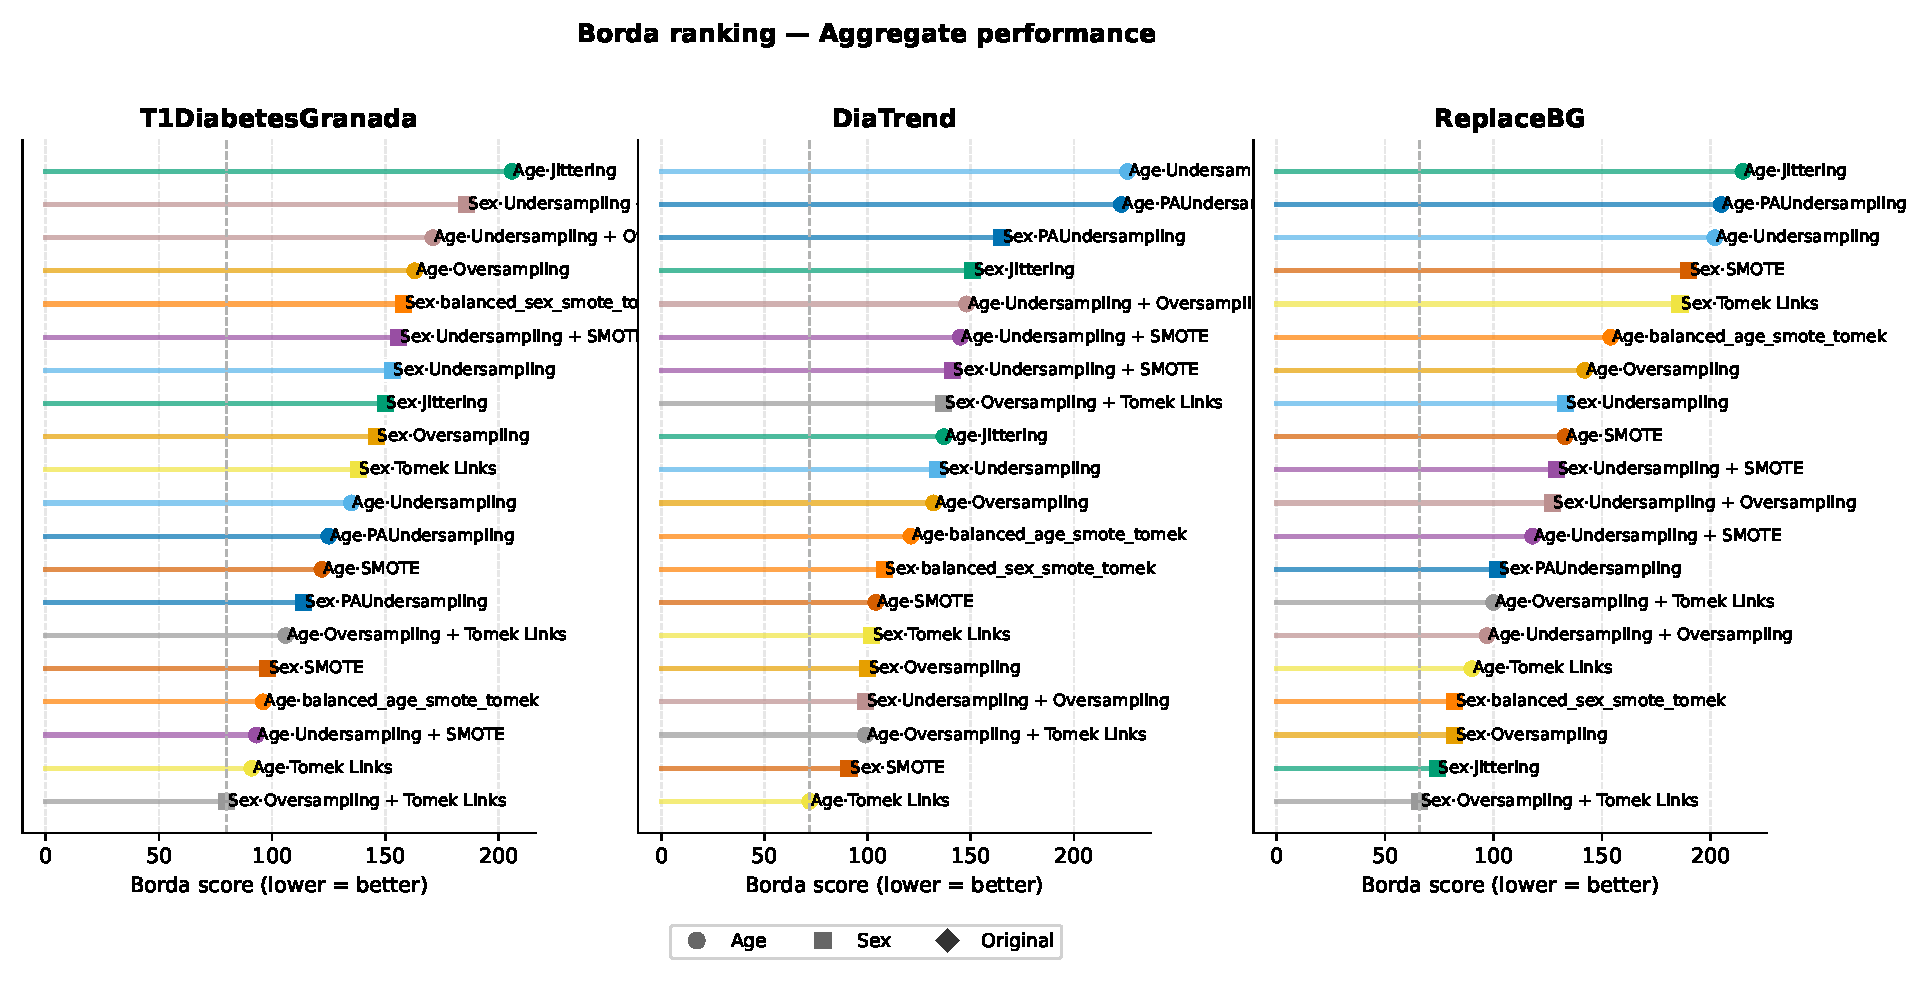
\includegraphics[width=0.85\textwidth]{%
        ../../analysis_relief/outputs/figures/rankings/borda_lollipop}
    \caption{Ranking global de técnicas mediante el método Borda (suma
             de posiciones de ranking a través de \textit{datasets},
             métricas y rangos glucémicos). Una puntuación Borda más baja
             indica mejor posicionamiento global. La línea discontinua
             vertical indica la puntuación del \textit{baseline} original
             en cada \textit{dataset}.}
    \label{fig:borda_lollipop}
\end{figure}

\begin{figure}[H]
    \centering
    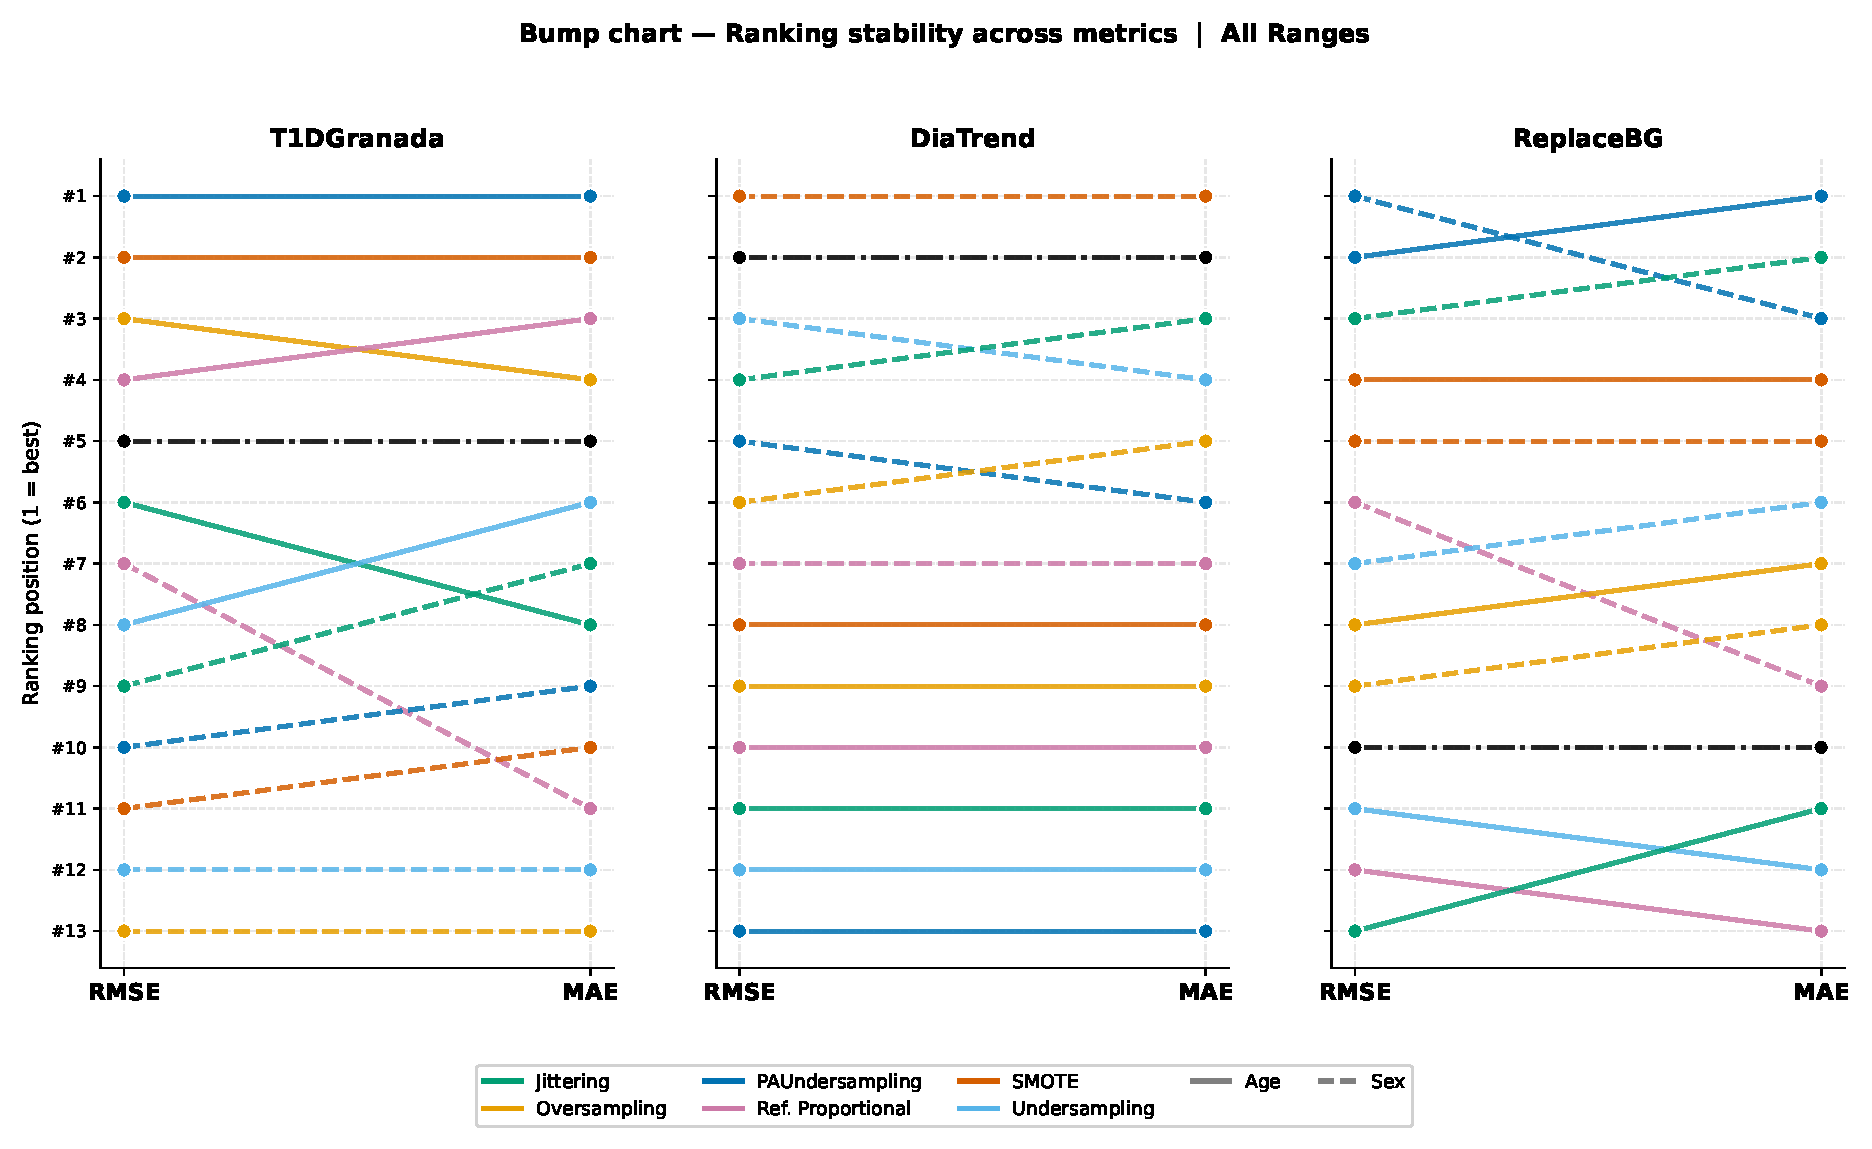
\includegraphics[width=\textwidth]{%
        ../../analysis_relief/outputs/figures/rankings/bump_chart_ENTIRE}
    \caption{\textit{Bump chart} mostrando la estabilidad del ranking
             de cada técnica entre RMSE y MAE para el conjunto completo
             (\textit{ENTIRE}), por \textit{dataset}. Líneas horizontales
             indican estabilidad del ranking entre métricas; líneas muy
             inclinadas indican que la técnica se comporta de forma
             diferente según la métrica utilizada.}
    \label{fig:bump_chart_entire}
\end{figure}

\paragraph{Ranking Borda y estabilidad entre métricas.}
El \textit{lollipop} de Borda de la figura~\ref{fig:borda_lollipop}
agrega el rendimiento a través de todos los rangos glucémicos y revela
que \textbf{ninguna técnica es consistentemente la mejor en los tres
repositorios simultáneamente}. En T1DiabetesGranada Age·Jittering
obtiene la puntuación Borda más baja (mejor posicionamiento agregado),
seguida de Sex·Undersampling y Age·Undersampling+Oversampling, mientras
que Sex·Oversampling+Tomek Links es la peor posicionada. En DiaTrend el
ranking se invierte dramáticamente: Age·Undersampling y
Age·PAUndersampling lideran (puntuaciones Borda $<100$, posiciones
altas en rangos de hipoglucemia), mientras que Age·Tomek Links cae a
la última posición, la opuesta a su liderazgo en el CD diagram de ENTIRE.
En REPLACE-BG Age·Jittering coincide con T1DiabetesGranada en liderar
el Borda, seguida de Age·PAUndersampling y Age·Undersampling, con
Sex·Oversampling+Tomek Links en última posición en los tres repositorios.

El \textit{bump chart} de la figura~\ref{fig:bump_chart_entire} añade
la perspectiva de la estabilidad entre métricas (RMSE vs.\ MAE).
En \textbf{DiaTrend} las líneas son prácticamente horizontales para
todas las técnicas, lo que indica que el ranking por RMSE y por MAE
es casi idéntico: la elección de la métrica de error no altera las
conclusiones en este repositorio. En \textbf{T1DiabetesGranada} hay
algunos cruzamientos notables: Age·PAUndersampling (posición 1 en RMSE)
desciende a posición 5 en MAE, y Age·Oversampling sube de posición 20
en RMSE a posición 8 en MAE, lo que sugiere que algunas técnicas tienen
un perfil de error asimétrico (cometen errores grandes en pocos casos
vs.\ errores pequeños distribuidos). En \textbf{REPLACE-BG} la
inestabilidad es la más pronunciada de los tres: varios cruzamientos
indican que el ranking entre técnicas depende de la métrica elegida,
coherente con la baja consistencia inter-fold ya observada en la
figura~\ref{fig:consistency_folds}.

En conjunto, los resultados estadísticos de esta subsección establecen
tres conclusiones definitivas. Primera: \textbf{solo en DiaTrend existe
evidencia estadística de que el balanceo modifica el rendimiento del
modelo} de forma reproducible entre folds; en T1DiabetesGranada y
REPLACE-BG las diferencias observadas son estadísticamente compatibles
con variación aleatoria. Segunda: \textbf{en DiaTrend el efecto es
estadísticamente significativo en todos los rangos glucémicos}, pero el
ranking óptimo de técnicas depende del rango que se priorice: las
técnicas que lideran en ENTIRE deterioran TBR-2 y viceversa. Tercera:
\textbf{no existe ninguna técnica universalmente óptima}: la elección
debe hacerse en función del repositorio, el rango glucémico de interés
clínico y la métrica de evaluación prioritaria.


% =========================================================
\section{Discusión integradora}
\label{sec:discusion}
% =========================================================

Esta sección sintetiza los hallazgos de las secciones anteriores y
responde de forma directa a las preguntas de investigación que motivaron
el trabajo. Cada respuesta integra la evidencia del análisis del
\textit{train set} (sección~\ref{sec:efecto_balanceo_trainset}) con la
del análisis de predicción (sección~\ref{sec:analisis_mejora}), y
distingue entre mejora estadística y relevancia clínica cuando ambas
dimensiones no coinciden.

\paragraph{¿Mejora el balanceo demográfico el rendimiento del modelo LSTM?}

La respuesta es matizada y fuertemente dependiente del repositorio y
del rango glucémico que se priorice. En términos globales (RMSE sobre
ENTIRE), el balanceo demográfico no produce mejoras estadísticamente
significativas en T1DiabetesGranada ($p = 0{,}120$, Friedman) ni en
REPLACE-BG ($p = 0{,}140$): en ambos repositorios las diferencias
observadas entre técnicas son estadísticamente compatibles con variación
aleatoria, y la evidencia de que cualquier técnica de balanceo supere al
\textit{baseline} original es insuficiente. En DiaTrend, en cambio, el
test de Friedman rechaza la hipótesis nula en todos los rangos y métricas
evaluados ($p < 0{,}0001$ en ENTIRE RMSE), y el post-hoc de Nemenyi
identifica grupos de técnicas estadísticamente distintos: las técnicas de
submuestreo agresivo por edad (RUS, PA-Undersampling) deterioran
significativamente el rendimiento global respecto a Tomek Links y a las
técnicas de dimensión sexo, mientras que estas últimas son
estadísticamente equivalentes al \textit{baseline}.

La lectura cambia al focalizar la evaluación en TBR-2 (hipoglucemia
severa, $<$54\,mg/dL), el rango clínicamente más crítico. En DiaTrend,
donde el test de Friedman también es significativo en TBR-2
($p = 0{,}00013$), el ranking se invierte: las técnicas de aumento
(ROS, SMOTE, ROS+Tomek) mejoran el RMSE en TBR-2 respecto al
\textit{baseline}, mientras que las de submuestreo lo empeoran. Esta
inversión sistemática confirma un \textbf{trade-off estructural}: en
DiaTrend no existe ninguna técnica que mejore simultáneamente el RMSE
global y el RMSE en hipoglucemia severa, lo que obliga a elegir entre
optimizar para el rendimiento medio o para el rango clínicamente más
prioritario. En T1DiabetesGranada y REPLACE-BG este trade-off existe en
los datos pero no alcanza significación estadística en ningún rango, por
lo que no puede afirmarse que el balanceo produzca un efecto clínico
neto demostrable en esos repositorios.

\paragraph{¿Qué familia de técnicas ofrece mejor relación beneficio/coste?}

El análisis por familia de tamaño
(sección~\ref{subsec:analisis_family_size}) demuestra que el volumen del
conjunto de entrenamiento no es el factor determinante del rendimiento
en T1DiabetesGranada ni en REPLACE-BG: las tres familias
(\textit{oversampling}, \textit{same\_size}, \textit{undersampling})
producen resultados estadísticamente equivalentes, lo que implica que
cualquier efecto positivo observado en esos repositorios debe atribuirse
al reequilibrio demográfico y no al cambio de tamaño del \textit{train}.
En DiaTrend, donde el efecto volumétrico es más pronunciado, Tomek Links
---que reduce el tamaño de forma moderada y selectiva, eliminando únicamente
puntos fronterizos--- obtiene el mejor RMSE global sin deteriorar TBR-2,
lo que lo posiciona como la técnica con mejor relación beneficio/coste
en ese repositorio.

Las técnicas \textit{same\_size} (RUS+ROS, RUS+SMOTE, SMOTE+Tomek)
ofrecen la ventaja de eliminar el confundidor volumétrico por diseño,
pero en ningún repositorio superan consistentemente a la mejor técnica
de su familia hermana: la compensación interna entre submuestreo y
sobremuestreo tiende a cancelar parcialmente los efectos de ambos
mecanismos, produciendo un perfil de rendimiento intermedio pero no
óptimo. Las técnicas de \textit{oversampling} puro son las que presentan
mayor riesgo de redundancia de datos en datasets pequeños y
desequilibrados como DiaTrend, donde la replicación del grupo $\geq$66
hasta $\approx$95 veces introduce una forma severa de sobreajuste latente
que el RMSE global no captura pero que puede manifestarse en métricas
de robustez fuera de la validación cruzada.

\paragraph{¿Es el efecto del balanceo \textit{dataset}-dependiente?}

Sí, de forma clara e inesperada en su magnitud. Los tres repositorios
evaluados representan tres escenarios estructuralmente distintos que
producen respuestas radicalmente diferentes al mismo conjunto de técnicas:

T1DiabetesGranada es el repositorio con mayor volumen (736 pacientes,
$\approx$13{,}6 millones de ventanas de \textit{train}) y un desequilibrio
demográfico por edad moderado (3{,}4:1). La alta consistencia relativa de
los seguimientos y la abundancia de datos hacen que el modelo LSTM ya
disponga de suficiente información con la partición original: cualquier
modificación del conjunto de entrenamiento produce cambios en la
composición glucémica inferiores al $1\%$ (sección~\ref{subsec:impacto_glucemico})
y ninguna mejora estadísticamente detectable en el rendimiento. El test
de Friedman no rechaza la hipótesis nula en ningún rango, lo que sugiere
que en repositorios grandes con desequilibrio moderado el balanceo
demográfico es innecesario desde el punto de vista predictivo.

REPLACE-BG es el repositorio más homogéneo: sus seguimientos estandarizados
de $\approx$182 días eliminan la heterogeneidad inter-paciente que amplifica
el desequilibrio en los otros dos datasets. Esta homogeneidad hace que el
balanceo demográfico produzca cambios mínimos tanto en la composición del
\textit{train} como en el rendimiento del modelo, y el test de Friedman no
rechaza la hipótesis nula en ningún rango ni métrica. REPLACE-BG ilustra
un escenario en que el diseño controlado del estudio previene el problema
que el balanceo intenta corregir, convirtiendo las técnicas de reequilibrio
en intervenciones superfluas.

DiaTrend es el caso más complejo: con solo 54 pacientes, un desequilibrio
etario de 38:1 a nivel de paciente que se amplifica hasta proporciones
extremas a nivel de ventana, y seguimientos muy heterogéneos (de semanas
a más de cinco años), es el único repositorio donde el balanceo produce
efectos estadísticamente detectables. Sin embargo, esos efectos son
ambivalentes: las técnicas que mejoran el rendimiento global deterioran
la hipoglucemia, y la alta variabilidad inter-fold (correlaciones de
Spearman inter-fold de $0{,}78$--$0{,}92$ en el ranking, pero con RMSE
que varía hasta $\pm$5\,mg/dL entre folds para la misma técnica)
advierte de que los resultados son inestables y difícilmente generalizables
más allá de este conjunto específico de pacientes.

\paragraph{¿Qué dimensión demográfica ---edad o sexo--- es más relevante?}

La dimensión edad produce efectos sistemáticamente más pronunciados que
la dimensión sexo en todos los repositorios y métricas evaluados. El
gráfico de pendientes de la figura~\ref{fig:slope_rmse_dim} muestra que
en DiaTrend las técnicas de edad producen una dispersión de
$\approx$3\,mg/dL en RMSE (desde mejoras del $-3\%$ hasta deterioros
del $-7\%$), mientras que las de sexo se concentran en un rango de
$\approx$0{,}5\,mg/dL próximo al \textit{baseline}. En T1DiabetesGranada
y REPLACE-BG ambas dimensiones producen efectos similares en magnitud,
pero las técnicas de edad presentan mayor variabilidad inter-fold,
coherente con el mayor ratio de desequilibrio de esa dimensión
(hasta 38:1 en DiaTrend frente a 2{,}2:1 en sexo).

La explicación estructural de esta diferencia reside en que el
desequilibrio por edad es más pronunciado, más correlacionado con el
perfil glucémico (los grupos etarios presentan distribuciones de TIR y
TAR distintas, como documentó el EDA en la sección~\ref{subsec:eda_cgm})
y más amplificado al pasar de nivel de paciente a nivel de ventana
(por las diferencias en duración de seguimiento entre grupos). El
desequilibrio por sexo, en cambio, es más moderado y menos correlacionado
con el perfil glucémico en estos repositorios ($\approx$42--59\,\% TIR
en ambos sexos, sección~\ref{subsec:eda_demografico}), lo que hace que
el balanceo por sexo tenga menos margen de impacto sobre lo que el
modelo aprende. Esta conclusión tiene implicaciones prácticas directas:
en futuros estudios con estos datasets, si se dispone de recursos
computacionales limitados, el balanceo por edad debe priorizarse sobre
el balanceo por sexo.

\paragraph{Limitaciones del análisis.}

Cuatro limitaciones principales deben considerarse al interpretar los
resultados de este trabajo. Primera, el número de \textit{folds} ($K=5$)
limita la potencia estadística del test de Friedman para detectar
diferencias pequeñas entre 21 condiciones: con solo 5 observaciones por
condición, la diferencia crítica de Nemenyi ($\text{CD} = 13{,}25$
posiciones de ranking) es tan amplia que puede enmascarar efectos reales
de magnitud moderada, especialmente en T1DiabetesGranada y REPLACE-BG.
Un esquema de validación cruzada con $K=10$ o la repetición de los
experimentos con múltiples semillas aleatorias aumentaría la sensibilidad
del análisis.

Segunda, DiaTrend tiene un tamaño muestral de 54 pacientes, insuficiente
para extraer conclusiones generalizables a otras poblaciones con diabetes
tipo 1. La alta variabilidad inter-fold documentada (sección~\ref{subsec:distribucion_metricas})
es consecuencia directa de este tamaño: con tan pocos pacientes, la
composición de cada \textit{fold} depende fuertemente de qué individuos
caen en el subconjunto de test, y los resultados son sensibles a esa
asignación. Los hallazgos estadísticamente significativos en DiaTrend
deben interpretarse como indicativos del potencial del balanceo en
datasets pequeños y desequilibrados, no como estimaciones robustas del
efecto poblacional.

Tercera, el análisis se restringe a un único modelo (LSTM) y un único
horizonte de predicción (PH$=4$, 60 minutos en DiaTrend). El efecto
del balanceo demográfico puede diferir para otros modelos (transformers,
modelos lineales, gradient boosting) o para horizontes más cortos o más
largos, dado que la distribución glucémica relevante para la predicción
cambia con el horizonte temporal.

Cuarta, el efecto del balanceo sobre el \textit{train set} se ha
cuantificado a nivel de distribución glucémica de las ventanas
(sección~\ref{sec:efecto_balanceo_trainset}), pero no se ha analizado
el impacto sobre las propiedades temporales de las series generadas:
la autocorrelación entre ventanas adyacentes, la estacionariedad local
o la distribución de las transiciones glucémicas pueden verse alteradas
por las técnicas de síntesis (SMOTE, Jittering), lo que podría modular
la capacidad del LSTM para capturar las dependencias temporales relevantes
de forma no capturada por el RMSE agregado.